\documentclass{oblivoir}
%%%Default packages
\usepackage{amsmath,amssymb,amsthm,kotex,tabu,graphicx,pifont}
\usepackage{../kswrapfig}

\usepackage{gensymb} %\degree

%%%More packages
%\usepackage{caption,subcaption}
%\usepackage[perpage]{footmisc}
%
\usepackage[skipabove=10pt,innertopmargin=10pt,nobreak=true]{mdframed}

\usepackage[inline]{enumitem}
\setlist[enumerate,1]{label=(\arabic*)}
\setlist[enumerate,2]{label=(\alph*)}

\usepackage{multicol}
\setlength{\columnsep}{30pt}
\setlength{\columnseprule}{1pt}
%
%\usepackage{forest}
%\usetikzlibrary{shapes.geometric,arrows.meta,calc}
%
%%%defi theo exam prob rema proo
%이 환경들 아래에 문단을 쓸 경우 살짝 들여쓰기가 되므로 \hspace{-.7em}가 필요할 수 있다.

\newcounter{num}
\newcommand{\defi}[1]
{\noindent\refstepcounter{num}\textbf{정의 \arabic{num})} #1\par\noindent}
\newcommand{\theo}[1]
{\noindent\refstepcounter{num}\textbf{정리 \arabic{num})} #1\par\noindent}
\newcommand{\revi}[1]
{\noindent\refstepcounter{num}\textbf{복습 \arabic{num})} #1\par\noindent}
\newcommand{\exam}[1]
{\bigskip\bigskip\noindent\refstepcounter{num}\textbf{예시 \arabic{num})} #1\par\noindent}
\newcommand{\prob}[1]
{\bigskip\bigskip\noindent\refstepcounter{num}\textbf{문제 \arabic{num})} #1\par\noindent}
\newcommand{\rema}[1]
{\bigskip\bigskip\noindent\refstepcounter{num}\textbf{참고 \arabic{num})} #1\par\noindent}
\newcommand{\proo}
{\bigskip\noindent\textsf{증명)}}

\newenvironment{talign}
 {\let\displaystyle\textstyle\align}
 {\endalign}
\newenvironment{talign*}
 {\let\displaystyle\textstyle\csname align*\endcsname}
 {\endalign}
%
%%%Commands

\newcommand{\procedure}[1]{\begin{mdframed}\vspace{#1\textheight}\end{mdframed}}

\newcommand\an[1]{\par\bigskip\noindent\textbf{문제 \ref{#1})}\par\noindent}

\newcommand\ann[2]{\par\bigskip\noindent\textbf{문제 \ref{#1})}\:\:#2\par\medskip\noindent}

\newcommand\ans[1]{\begin{flushright}\textbf{답 : }#1\end{flushright}}

\newcommand\anssec[1]{\bigskip\bigskip\noindent{\large\bfseries#1}}

\newcommand{\pb}[1]%\Phantom + fBox
{\fbox{\phantom{\ensuremath{#1}}}}

\newcommand\ba{\,|\,}

\newcommand\ovv[1]{\ensuremath{\overline{#1}}}
\newcommand\ov[2]{\ensuremath{\overline{#1#2}}}
%
%%%% Settings
%\let\oldsection\section
%
%\renewcommand\section{\clearpage\oldsection}
%
%\let\emph\textsf
%
%\renewcommand{\arraystretch}{1.5}
%
%%%% Footnotes
%\makeatletter
%\def\@fnsymbol#1{\ensuremath{\ifcase#1\or
%*\or **\or ***\or
%\star\or\star\star\or\star\star\star\or
%\dagger\or\dagger\dagger\or\dagger\dagger\dagger
%\else\@ctrerr\fi}}
%
%\renewcommand{\thefootnote}{\fnsymbol{footnote}}
%\makeatother
%
%\makeatletter
%\AtBeginEnvironment{mdframed}{%
%\def\@fnsymbol#1{\ensuremath{\ifcase#1\or
%*\or **\or ***\or
%\star\or\star\star\or\star\star\star\or
%\dagger\or\dagger\dagger\or\dagger\dagger\dagger
%\else\@ctrerr\fi}}%
%}   
%\renewcommand\thempfootnote{\fnsymbol{mpfootnote}}
%\makeatother
%
%%% 객관식 선지
\newcommand\one{\ding{172}}
\newcommand\two{\ding{173}}
\newcommand\three{\ding{174}}
\newcommand\four{\ding{175}}
\newcommand\five{\ding{176}}
\usepackage{tabto,pifont}
%\TabPositions{0.2\textwidth,0.4\textwidth,0.6\textwidth,0.8\textwidth}

\newcommand\taba[5]{\par\noindent
\one\:{#1}
\tabto{0.2\textwidth}\two\:\:{#2}
\tabto{0.4\textwidth}\three\:\:{#3}
\tabto{0.6\textwidth}\four\:\:{#4}
\tabto{0.8\textwidth}\five\:\:{#5}}

\newcommand\tabb[5]{\par\noindent
\one\:{#1}
\tabto{0.33\textwidth}\two\:\:{#2}
\tabto{0.67\textwidth}\three\:\:{#3}\medskip\par\noindent
\four\:\:{#4}
\tabto{0.33\textwidth}\five\:\:{#5}}

\newcommand\tabc[5]{\par\noindent
\one\:{#1}
\tabto{0.5\textwidth}\two\:\:{#2}\medskip\par\noindent
\three\:\:{#3}
\tabto{0.5\textwidth}\four\:\:{#4}\medskip\par\noindent
\five\:\:{#5}}

\newcommand\tabd[5]{\par\noindent
\one\:{#1}\medskip\par\noindent
\two\:\:{#2}\medskip\par\noindent
\three\:\:{#3}\medskip\par\noindent
\four\:\:{#4}\medskip\par\noindent
\five\:\:{#5}}
%
%%%% fonts
%
%\usepackage{fontspec, xunicode, xltxtra}
%\setmainfont[]{은 바탕}
%\setsansfont[]{은 돋움}
%\setmonofont[]{은 바탕}
%\XeTeXlinebreaklocale "ko"
\DeclareSymbolFont{yhlargesymbols}{OMX}{yhex}{m}{n}
\DeclareMathAccent{\wideparen}{\mathord}{yhlargesymbols}{"F3}
\usepackage{multirow,multicol}
%%%%
\begin{document}

\title{수학Ⅰ : 04 삼각함수}
\author{}
\date{\today}
\maketitle
\tableofcontents
\newpage

%%%
\section{호도법}

%
\prob{단위 변환}\label{rad1}
`인치(in)'는  미국에서 주로 사용되는 길이 단위로 \(1\;\text{in}\)는 약 \(2,54\;\text{cm}\)에 해당한다.
\[1\;\text{in}\approx2.54\;\text{cm}\]
다음 빈 칸에 알맞은 숫자 혹은 식을 써넣으시오.
\begin{enumerate}
\item
\(3\;\text{in}\approx\pb{8.62}\;\text{cm}\)
\item
\(1\;\text{cm}\approx\pb{0.39}\;\text{in}\)
\item
\(4\;\text{cm}\approx\pb{0.91}\;\text{in}\)
\end{enumerate}

\bigskip\bigskip
지금까지 각의 크기를 나타낼 때, 30\textdegree{}, 90\textdegree{}, \(120\)\textdegree{}와 같이 도(\textdegree{})를 단위로 하는 육십분법을 사용하였다.
이제 각의 크기를 나타내는 새로운 단위를 알아보자.
\begin{mdframed}
%
\defi{호도법}\label{rad2}
반지름의 길이가 \(r\)이고 호의 길이도 \(r\)인 부채꼴의 중심각의 크기를\\ 1rad으로 정한다.
rad는 각을 나타내는 단위로 `라디안(radian)'이라고 읽는다.
%반지름의 길이가 1인 원에서 호의 길이가 \(\alpha\)인 부채꼴의 중심각의 크기를 \(\alpha\) 라디안(radian)이라고 한다.
\begin{center}
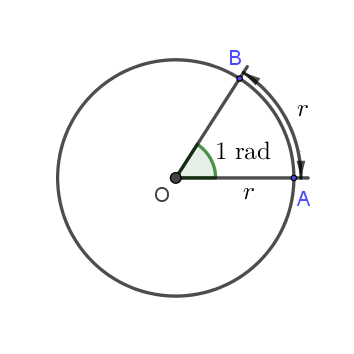
\includegraphics[width=.3\textwidth]{rad_2-1}
\qquad\qquad
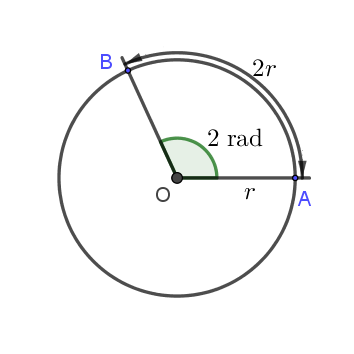
\includegraphics[width=.3\textwidth]{rad_2-2}
\end{center}
\end{mdframed}

\newpage
%
\rema{}
\begin{enumerate}\label{rad3}
\item
호의 길이는 중심각의 크기에 비례하므로
\(r:2\pi r=1\text{rad}:360\textdegree{}\)
이다.
따라서
\[1\text{rad}=\frac{180\textdegree{}}{\pi}\tag{$*$}\]
\(\pi\)의 값에 \(\pi=3.14\cdots\)을 대입하면 \(1\text{rad}\)은 약 \(57.29\textdegree{}\)정도이다.
\[1\text{rad}\approx57.29\textdegree{}\]
\item
\((*)\)의 양변에 \(\pi\)를 곱하면 \(\pi\;\text{rad}=180\textdegree{}\)이다.
%각의 크기를 호도법으로 나타낼 때에는
이때, 단위인 라디안은 생략하는 것이 보통이다.
따라서
\[\pi=180\textdegree{}\]
라고 쓴다.
\item
\(90\textdegree{}\)는 \(180\textdegree{}\)의 절반이므로
\(90\textdegree{}=\frac{\pi}2\)
이다.\\
\(30\textdegree{}\)는 \(180\textdegree{}\)의 \(\frac16\)이므로
\(30\textdegree{}=\frac{\pi}6\)
이다.\\
\(360\textdegree{}\)는 \(180\textdegree{}\)의 두 배이므로
\(360\textdegree{}=2\pi\)
이다.
\end{enumerate}

%
\prob{다음 표를 완성하여라.}\label{rad4}
\par\noindent
\begin{tabu}{|X[c$]|X[c$]|X[c$]|X[c$]|X[c$]|X[c$]|X[c$]|X[c$]|X[c$]|X[c$]|X[c$]|}
\hline
 0\textdegree{}
&30\textdegree{}
&45\textdegree{}
&
&90\textdegree{}
&120\textdegree{}
&
&150\textdegree{}
&180\textdegree{}
&270\textdegree{}
&360\textdegree{}
\\\hline
0
&\frac\pi6
&
&\frac\pi3
&\frac\pi2
&
&\frac34\pi
&
&\pi
&
&
\\\hline
\end{tabu}

%%
%\prob{다음 각도를 호도법으로 나타내시오.}
%\begin{enumerate}\label{rad4}
%\item
%반지름의 길이가 4인 원에서 호의 길이가 \(\frac3\pi\)인 부채꼴의 중심각의 크기
%\item
%반지름의 길이가 1인 원에서 호의 길이가 \(\frac\pi2\)인 부채꼴의 중심각의 크기
%\item
%1\textdegree{}
%\item
%3\textdegree{}
%\end{enumerate}

%%%
\section{부채꼴의 호의 길이와 넓이}
\begin{minipage}{.6\textwidth}
%
\prob{오른쪽 그림과 같이 반지름의 길이가 \(10\)이고 중심각의 크기가 \(45\)\textdegree{}인 부채꼴의 호의 길이 \(l\)과 넓이 \(S\)를 각각 구하여라.}\label{arc1}
\end{minipage}
\begin{minipage}{.3\textwidth}
\centering
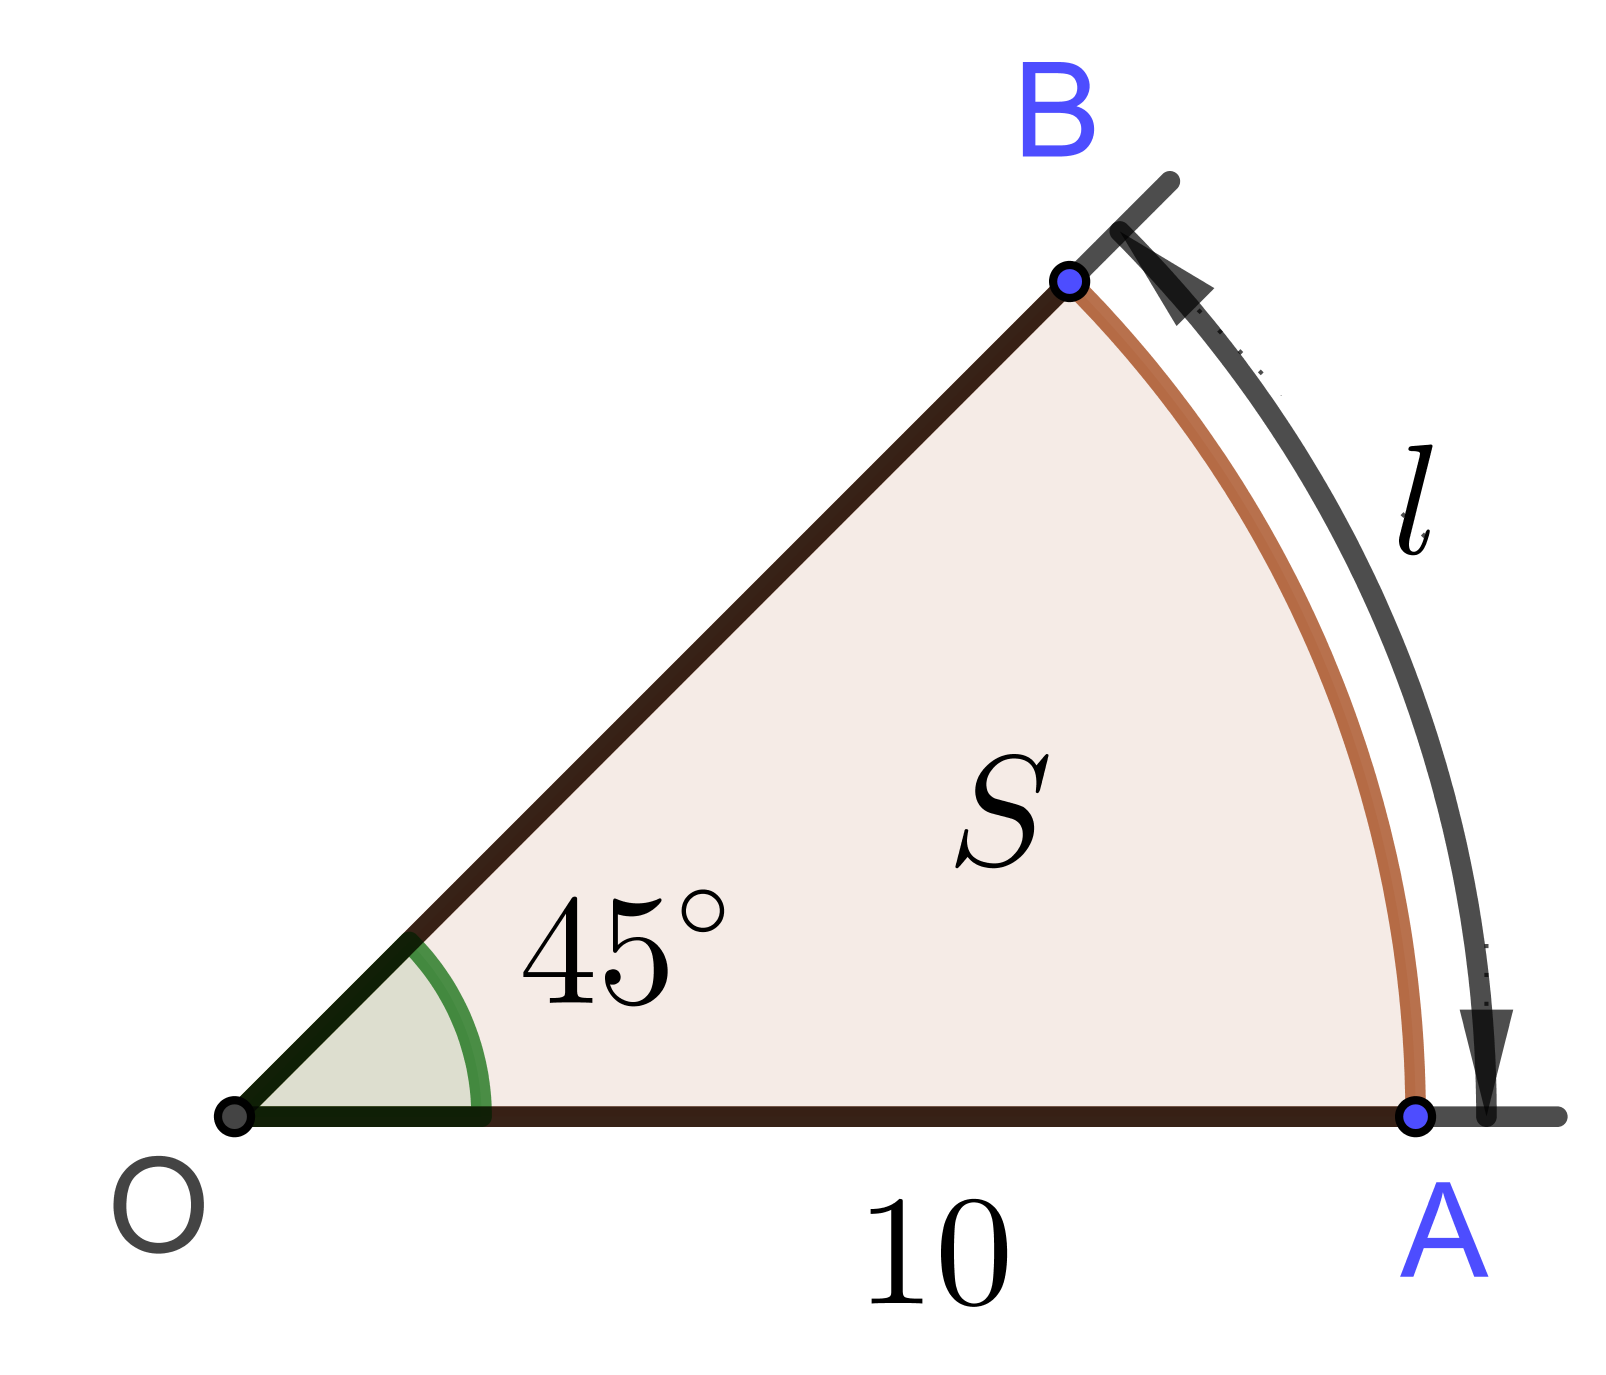
\includegraphics[width=.7\textwidth]{arc_1}
\end{minipage}

%
\rema{}\label{arc2}
위 문제에서 \(l\)과 \(S\)를 구하는 식은 각각
\begin{align*}
l&=2\pi\times10\times\frac{45}{360}\\
S&=\pi\times10^2\times\frac{45}{360}
\end{align*}
\noindent
\begin{minipage}{.6\textwidth}
이다.
이와 같은 원리를 이용하여, 이번에는\\ 반지름의 길이가 \(r\)이고 중심각의 크기가 \(\theta\)(rad)인 부채꼴의 호의 길이 \(l\)과 넓이 \(S\)를 구해보자.\footnotemark
\end{minipage}
\begin{minipage}{.3\textwidth}
\centering
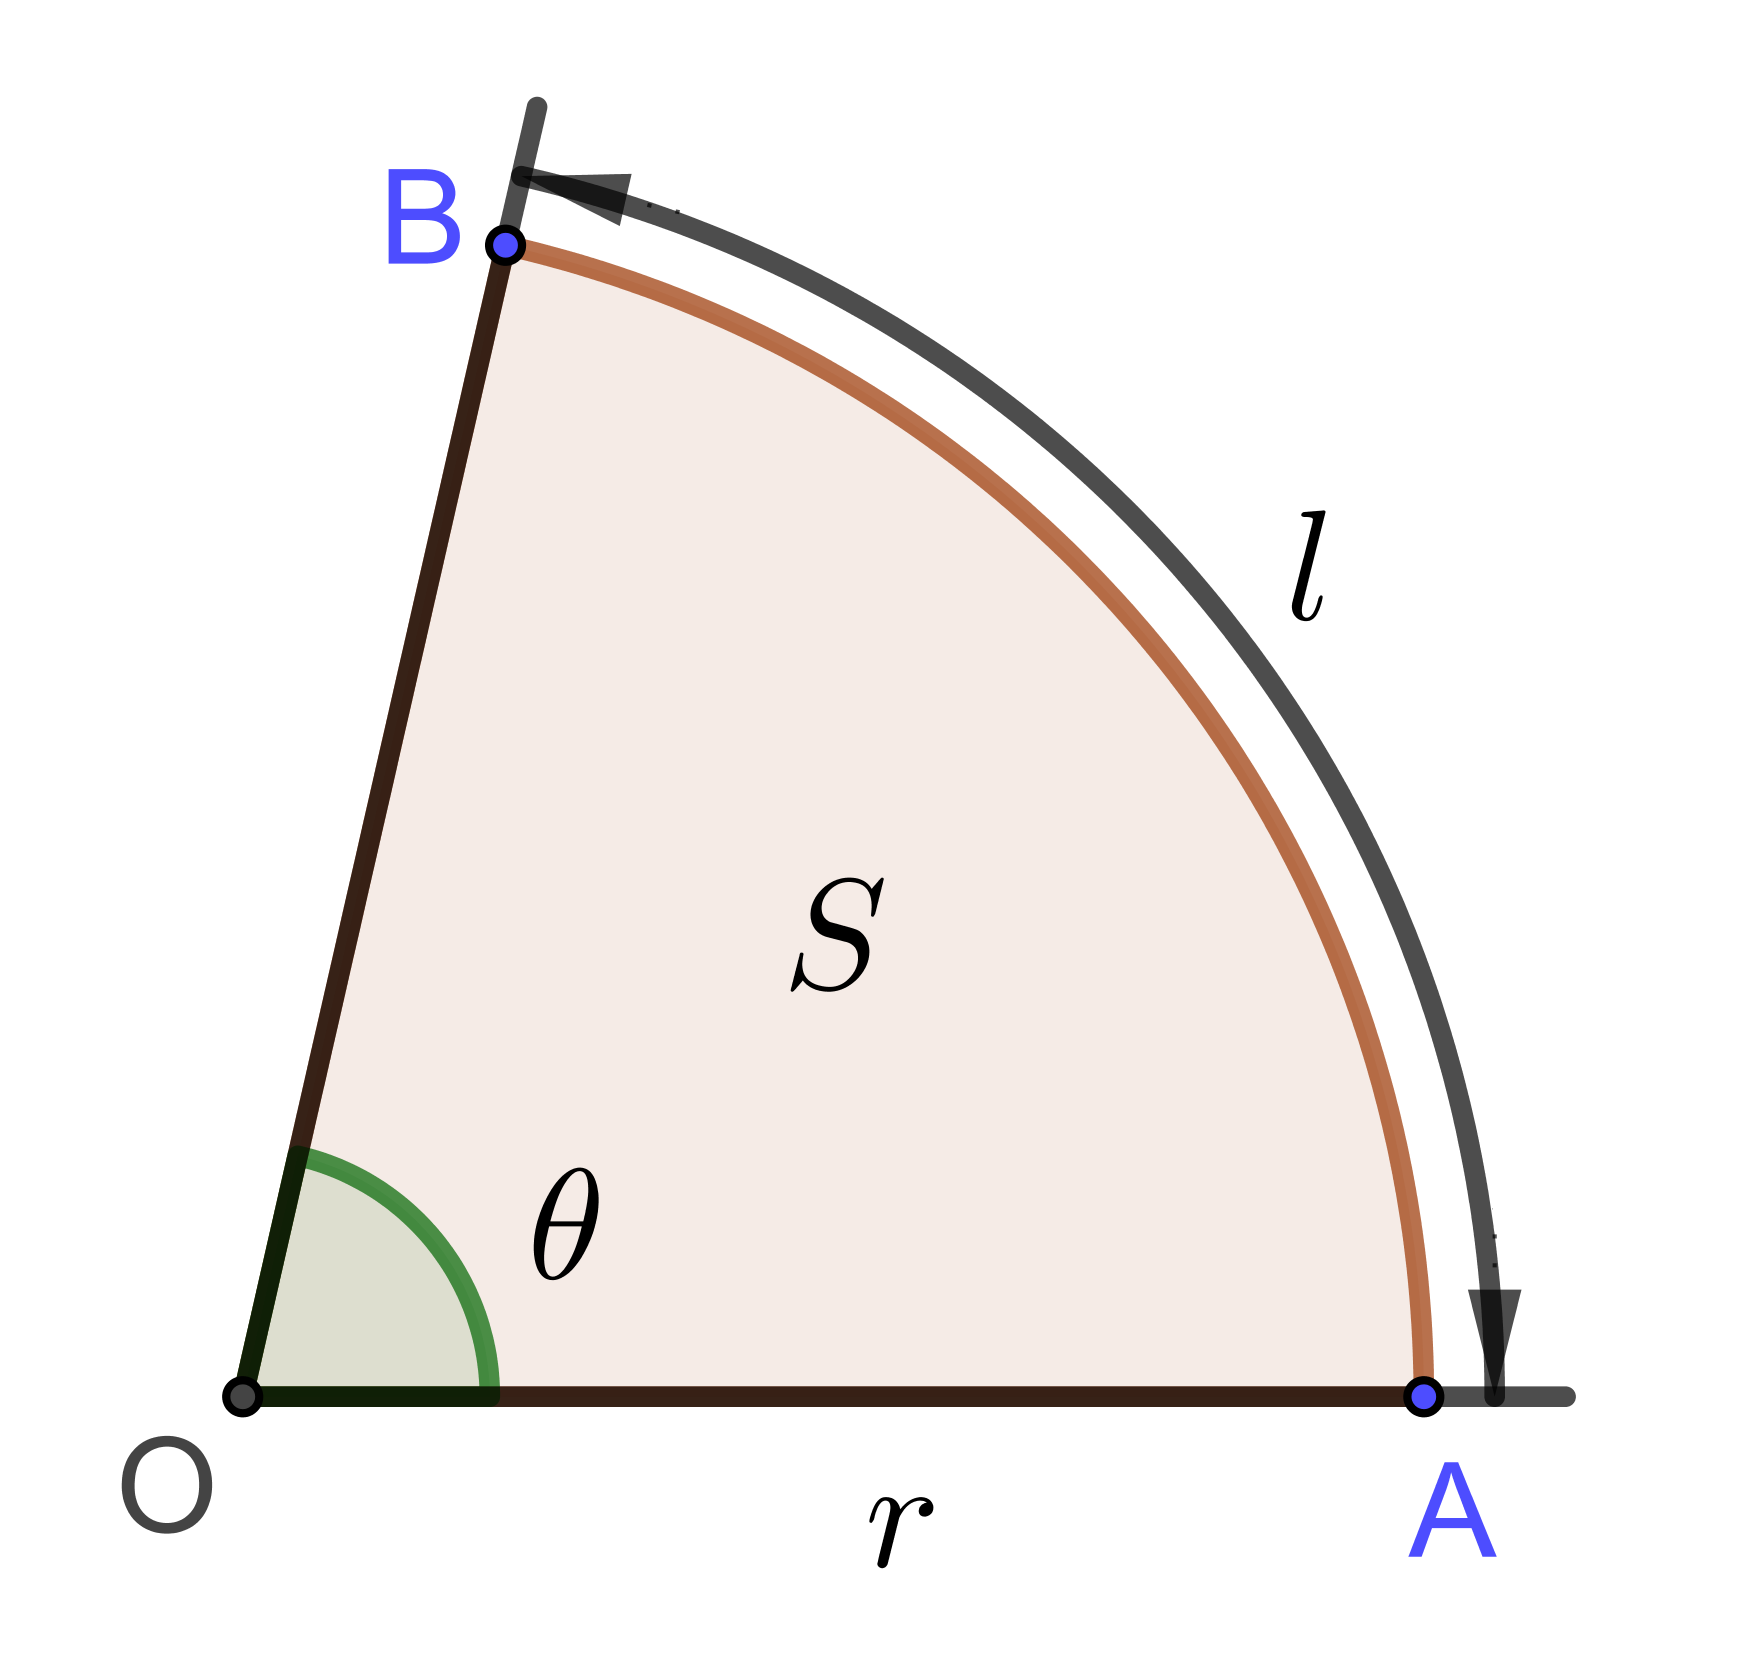
\includegraphics[width=.7\textwidth]{arc_2}
\end{minipage}
\footnotetext{\(\theta\)는 8번째 그리스어 문자로 세타(theta)라고 읽는다.
주로 각도를 표시할 때 쓰인다.}
%\begin{center}
%\includegraphics[width=.2\textwidth]{arc_5}
%\end{center}
\begin{align*}
l&=2\pi r\cdot\frac{\theta}{2\pi}\\
S&=\pi r^2\cdot\frac{\theta}{2\pi}
\end{align*}
따라서 \(l=r\theta\)이고 \(S=\frac12r^2\theta\)이다.
한편, \(S\)를 구하는 식을 조금 변형하면
\[S=\frac12r^2\theta=\frac12\times r\times r\theta=\frac12rl
%\pi r^2\cdot\frac{\theta}{2\pi}=2\pi r\cdot\frac{\theta}{2\pi}\times\frac12 r=l\times\frac12r=\frac12rl
\]
을 얻을 수도 있다.

\newpage\noindent
이것들을 정리하면 다음과 같다.
\begin{mdframed}
%
\theo{부채꼴의 호의 길이와 넓이}\label{arc3}
반지름의 길이가 \(r\)이고 중심각의 크기가 \(\theta\)(라디안)인 부채꼴의 호의 길이를 \(l\), 넓이를 \(S\)라고 하면\\
\begin{tabu}{X[c$]X[c$]X[c$]}
l=r\theta
&
S=\frac12r^2\theta
&
S=\frac12rl
\end{tabu}
\end{mdframed}

%
\exam{반지름의 길이가 4이고 중심각의 크기가 \(\frac34\pi\)인 부채꼴에서}\label{arc4}
\noindent
\begin{minipage}{.6\textwidth}
\begin{align*}
l&=4\times\frac34\pi=3\pi\\
S&=\frac12\times4^2\times\frac34\pi=6\pi
\end{align*}
\end{minipage}
\begin{minipage}{.3\textwidth}
\centering
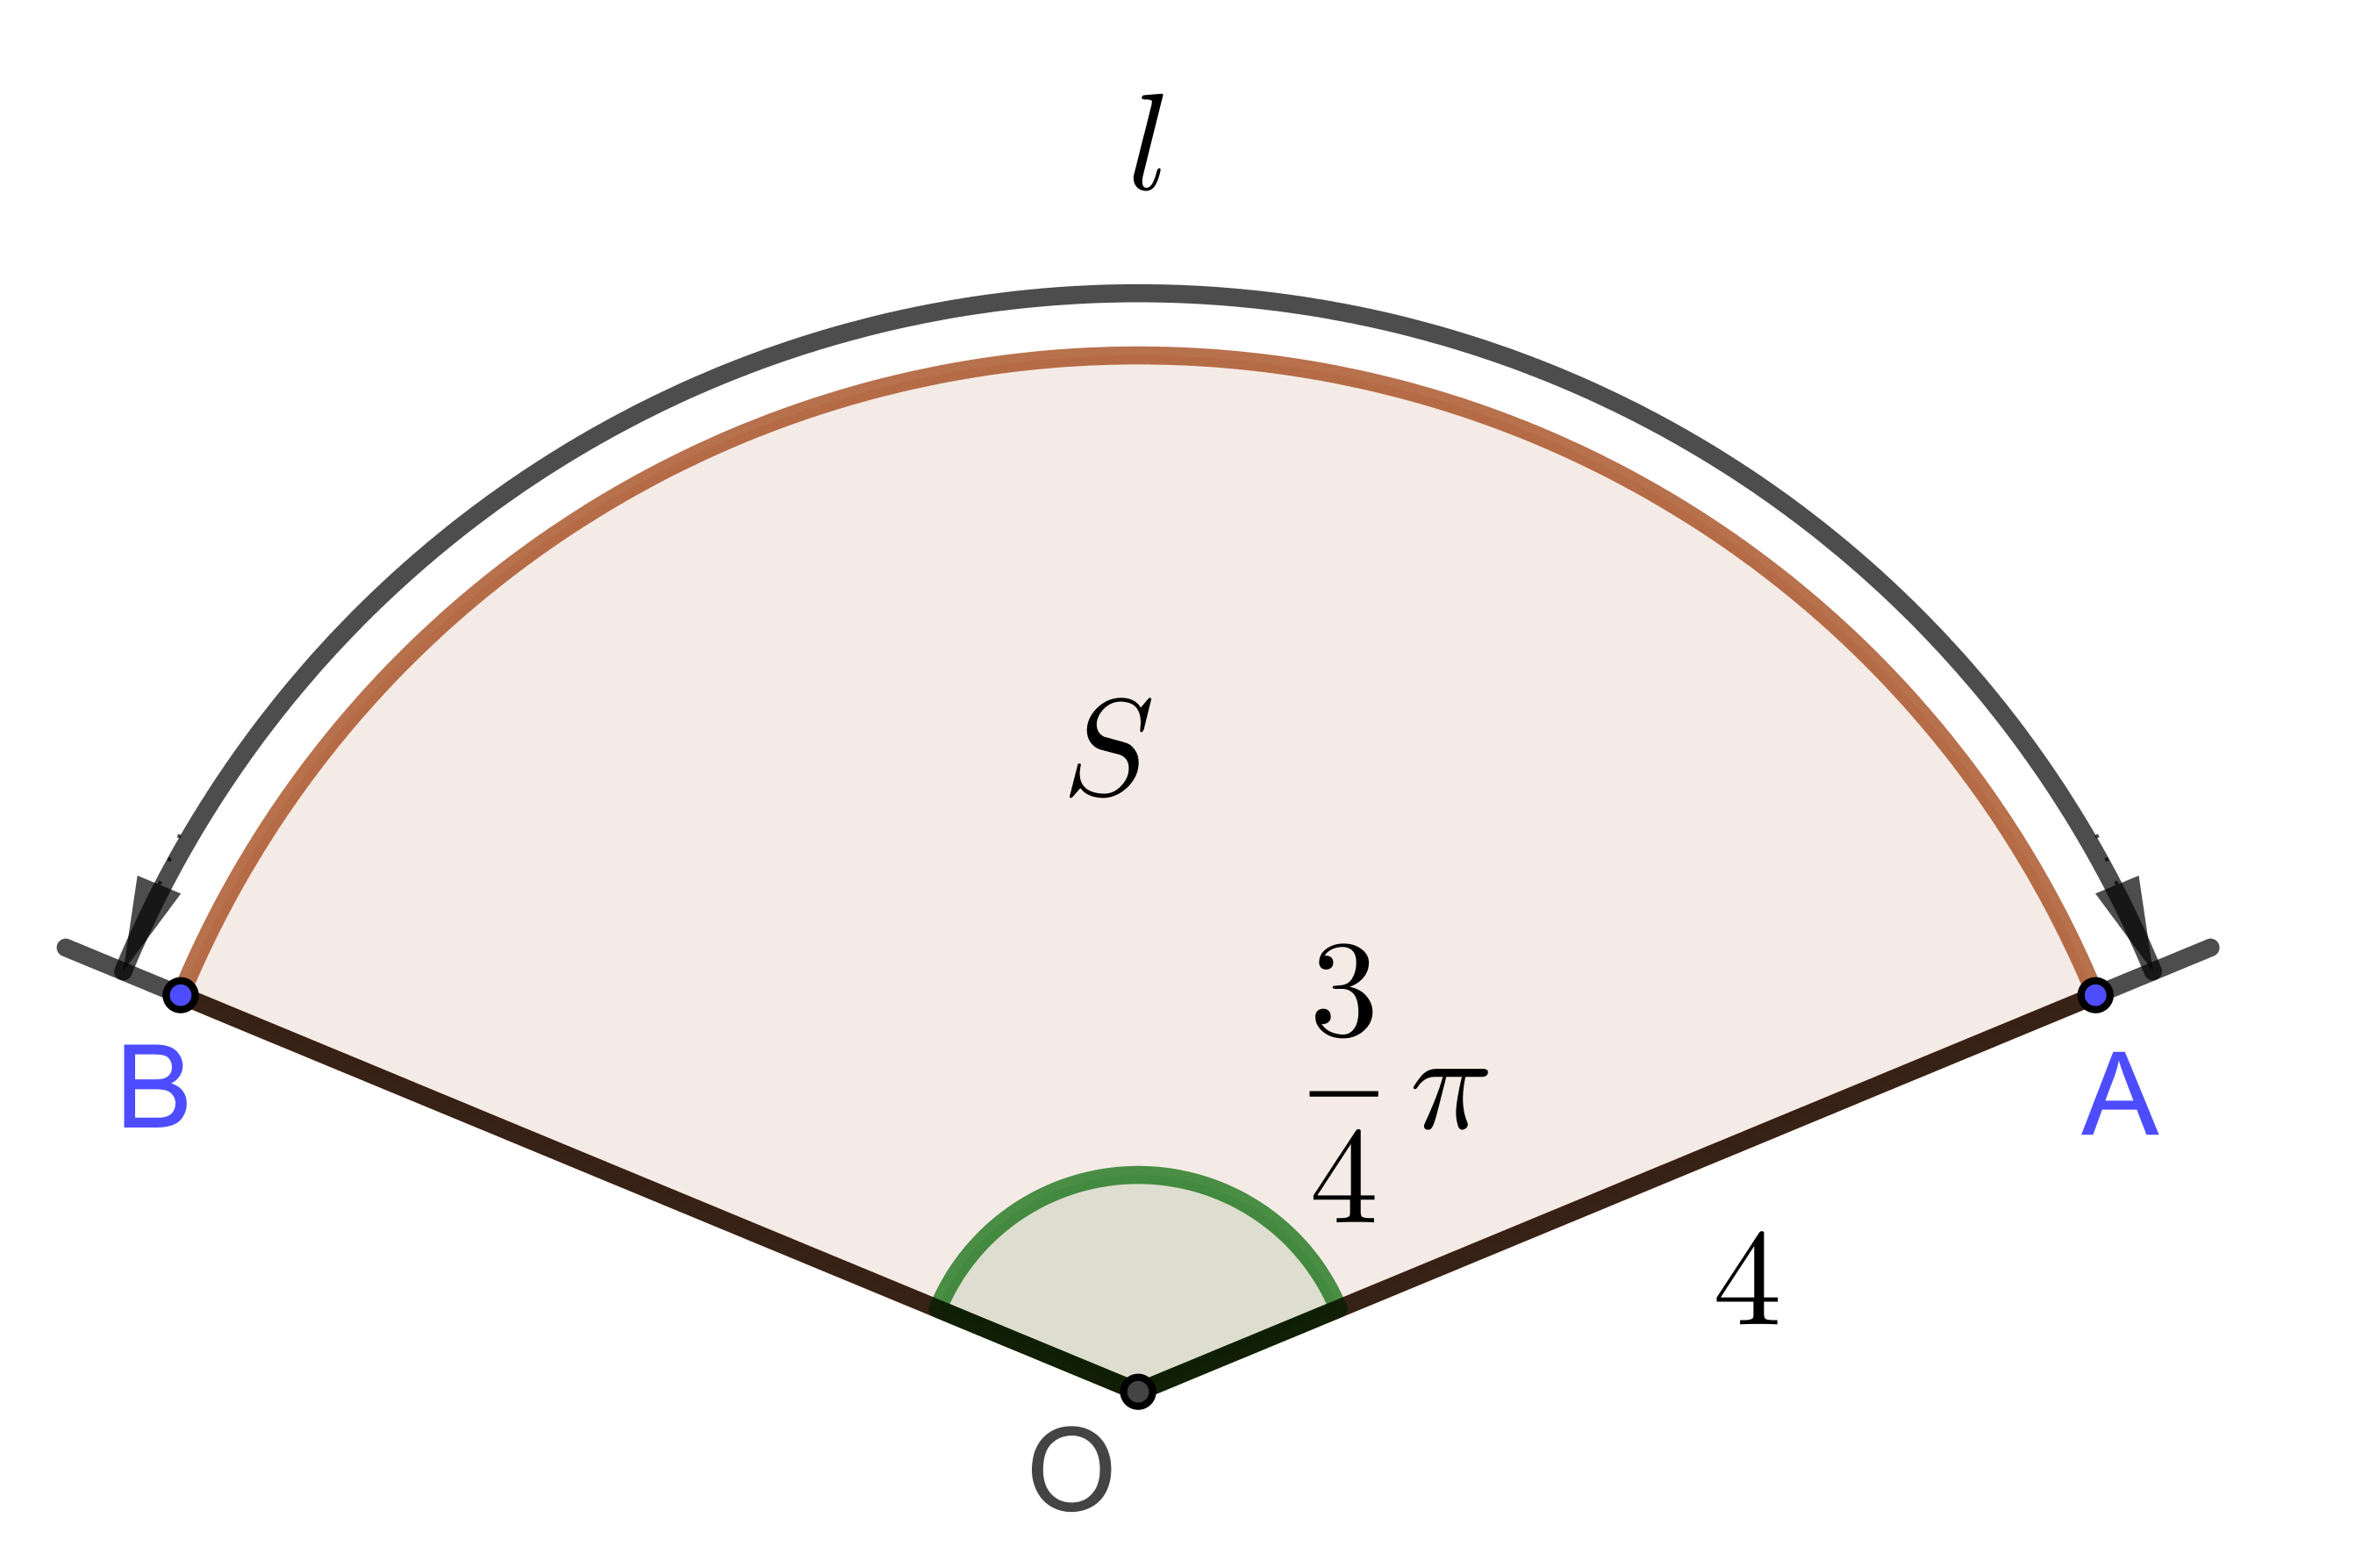
\includegraphics[width=\textwidth]{arc_4}
\end{minipage}

%
\prob{다음 부채꼴에서 호의 길이 \(l\)과 넓이 \(S\)를 구하여라.}
\begin{enumerate}\label{arc5}
\item
반지름의 길이가 6이고 중심각의 크기가 \(\frac\pi6\)인 부채꼴
\item
반지름의 길이가 10이고 중심각의 크기가 \(\frac23\pi\)인 부채꼴
\end{enumerate}

\vspace{30pt}
\noindent
\begin{minipage}{.6\textwidth}
%
\prob{호의 길이가 \(\pi\)이고 중심각의 크기가 \(\frac23\pi\)인 부채꼴의 넓이를 구하여라.}\label{arc6}
\end{minipage}
\begin{minipage}{.3\textwidth}
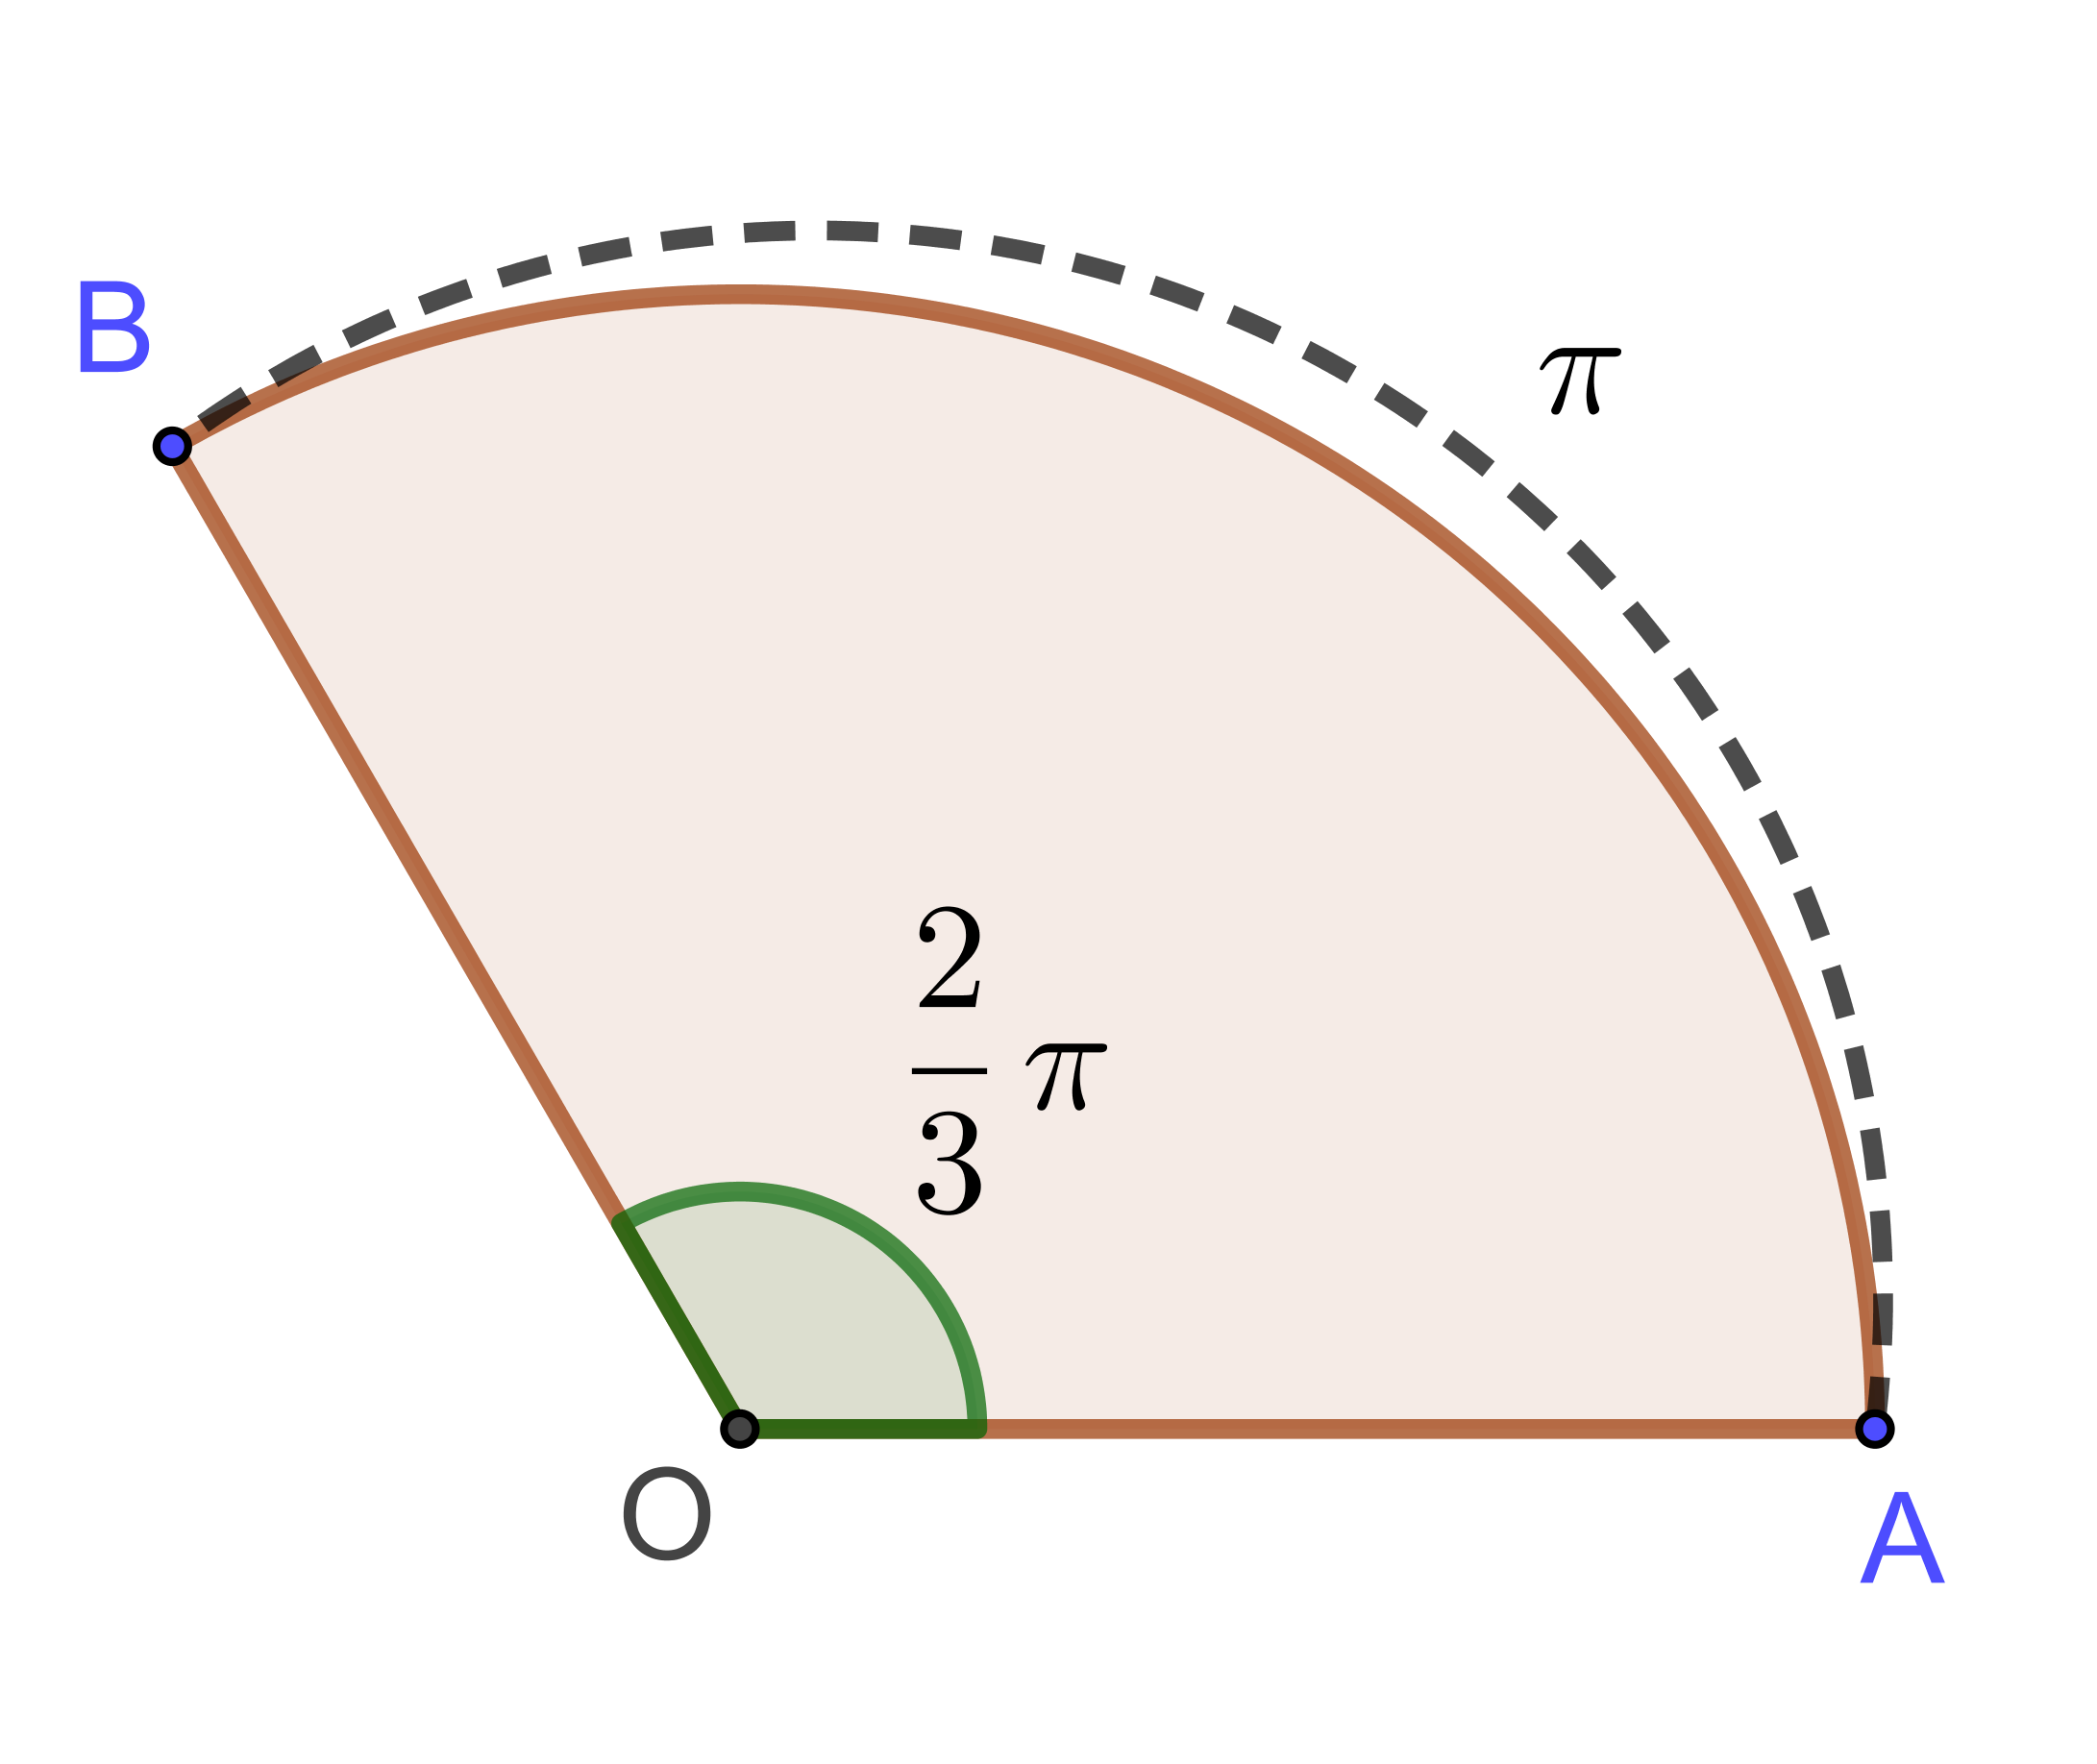
\includegraphics[width=.7\textwidth]{arc_6}
\end{minipage}

%%%
\section{복습(삼각비)}
\begin{mdframed}
%
\defi{삼각비}\label{tratio1}
\noindent\begin{minipage}{.6\textwidth}
%오른쪽 그림에서
\[\sin A=\frac ac,\quad\cos A=\frac bc,\quad\tan A=\frac ab\]
%이다.
\end{minipage}
\begin{minipage}{.4\textwidth}
\centering
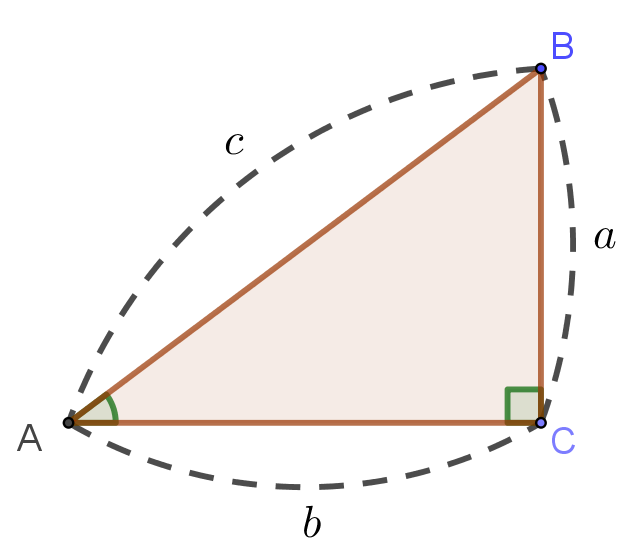
\includegraphics[width=.7\textwidth]{tratio_1}
\end{minipage}
\end{mdframed}

%
\exam{\(\frac\pi3=60\textdegree{}\)의 삼각비를 구하여라.}\label{tratio2}
\noindent\begin{minipage}{.6\textwidth}
오른쪽 그림에서
\[\sin\frac\pi3=\frac{\sqrt3}2,\quad\cos\frac\pi3=\frac12,\quad\tan\frac\pi3=\sqrt3\]
이다.
\end{minipage}
\begin{minipage}{.3\textwidth}
\centering
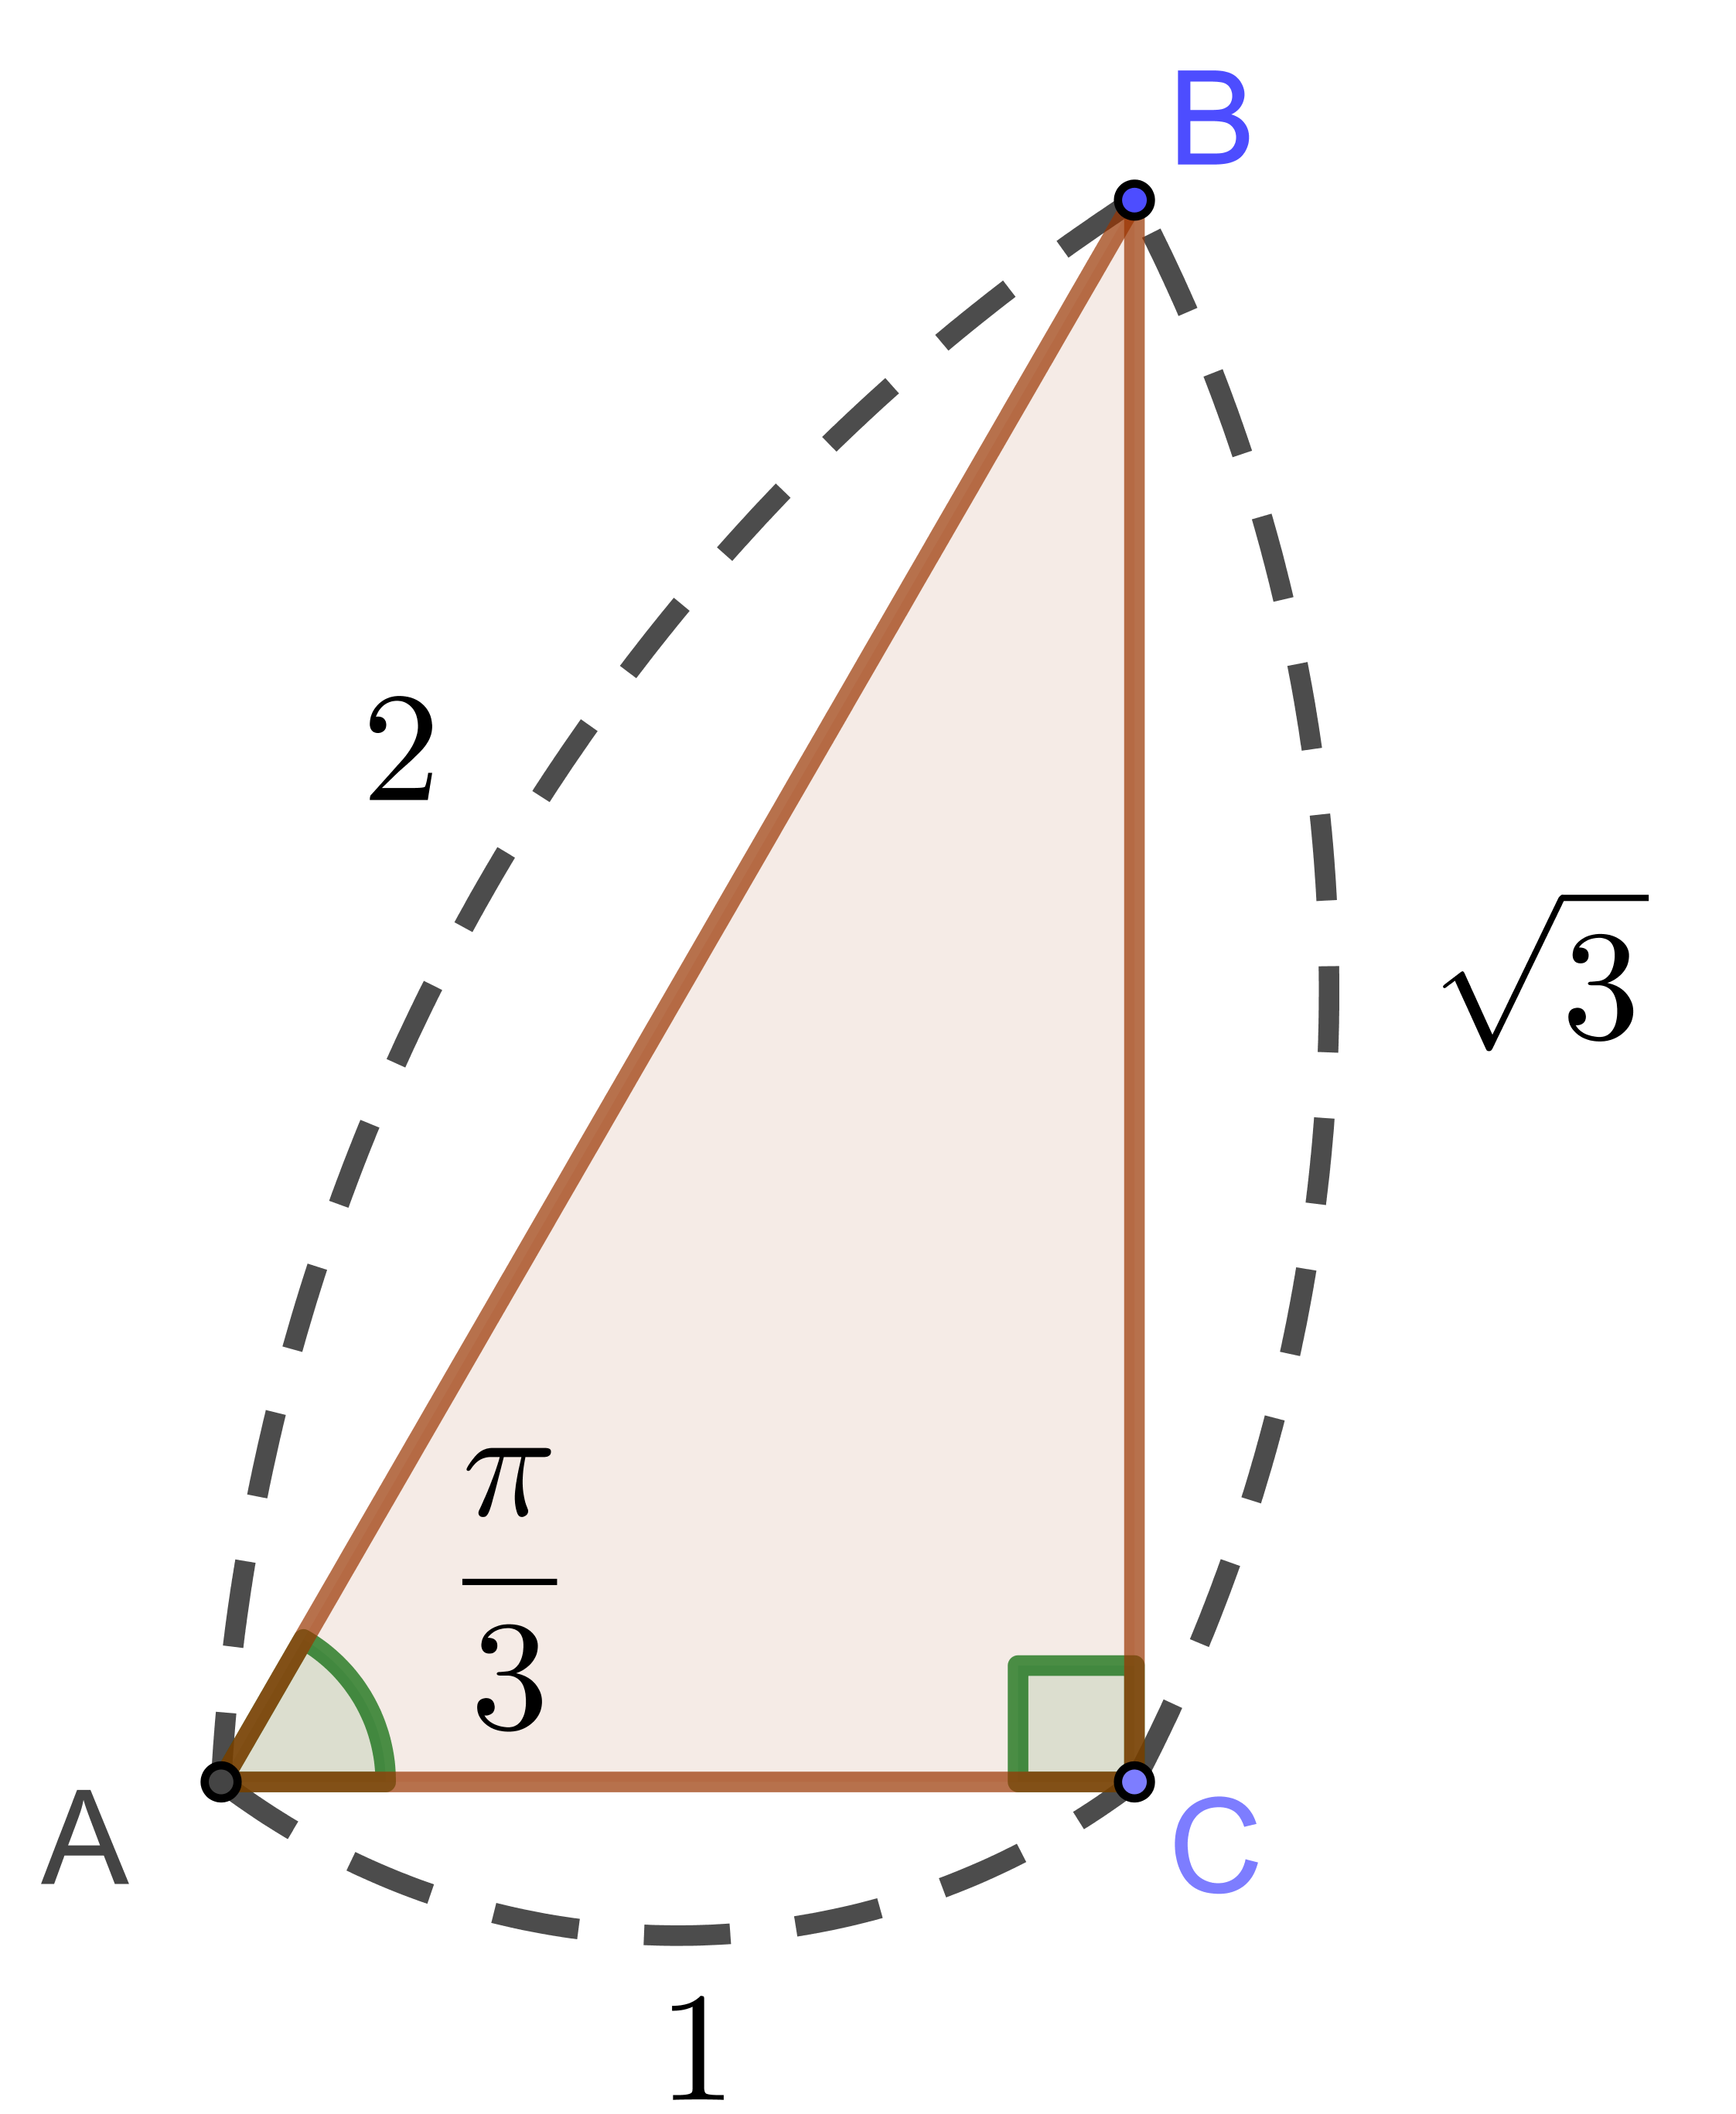
\includegraphics[width=.8\textwidth]{tratio_2}
\end{minipage}

%
\prob{다음 삼각비의 값들을 구하여라.}\label{tratio3}
\begin{center}
\begin{tabu}to.6\textwidth{X[$]X[$]X[$]}
(1)\;\;\sin\frac\pi6=&\cos\frac\pi6=&\tan\frac\pi6=\\
(2)\;\;\sin\frac\pi4=&\cos\frac\pi4=&\tan\frac\pi4=\\
\end{tabu}
\end{center}

%
\prob{다음 값을 계산하여라.}\label{tratio4}
\begin{talign*}
(\sin\frac\pi6)^2+(\cos\frac\pi6)^2&=\\
(\sin\frac\pi4)^2+(\cos\frac\pi4)^2&=\\
\end{talign*}

\newpage
\noindent
\begin{minipage}{.7\textwidth}
%
\prob{다음 그림에서 \(\wideparen{AB}\)는 중심이 원점이고 반지름이 1인 원의 일부이다.
\(\wideparen{AB}\)위의 한 점 \(P\)에 대하여 \(\angle POA=\theta\)라고 할 때, 다음 빈칸에 알맞은 선분을 써넣고 다음 물음에 답하여라.}
\label{tratio5}
\end{minipage}
\begin{minipage}{.3\textwidth}
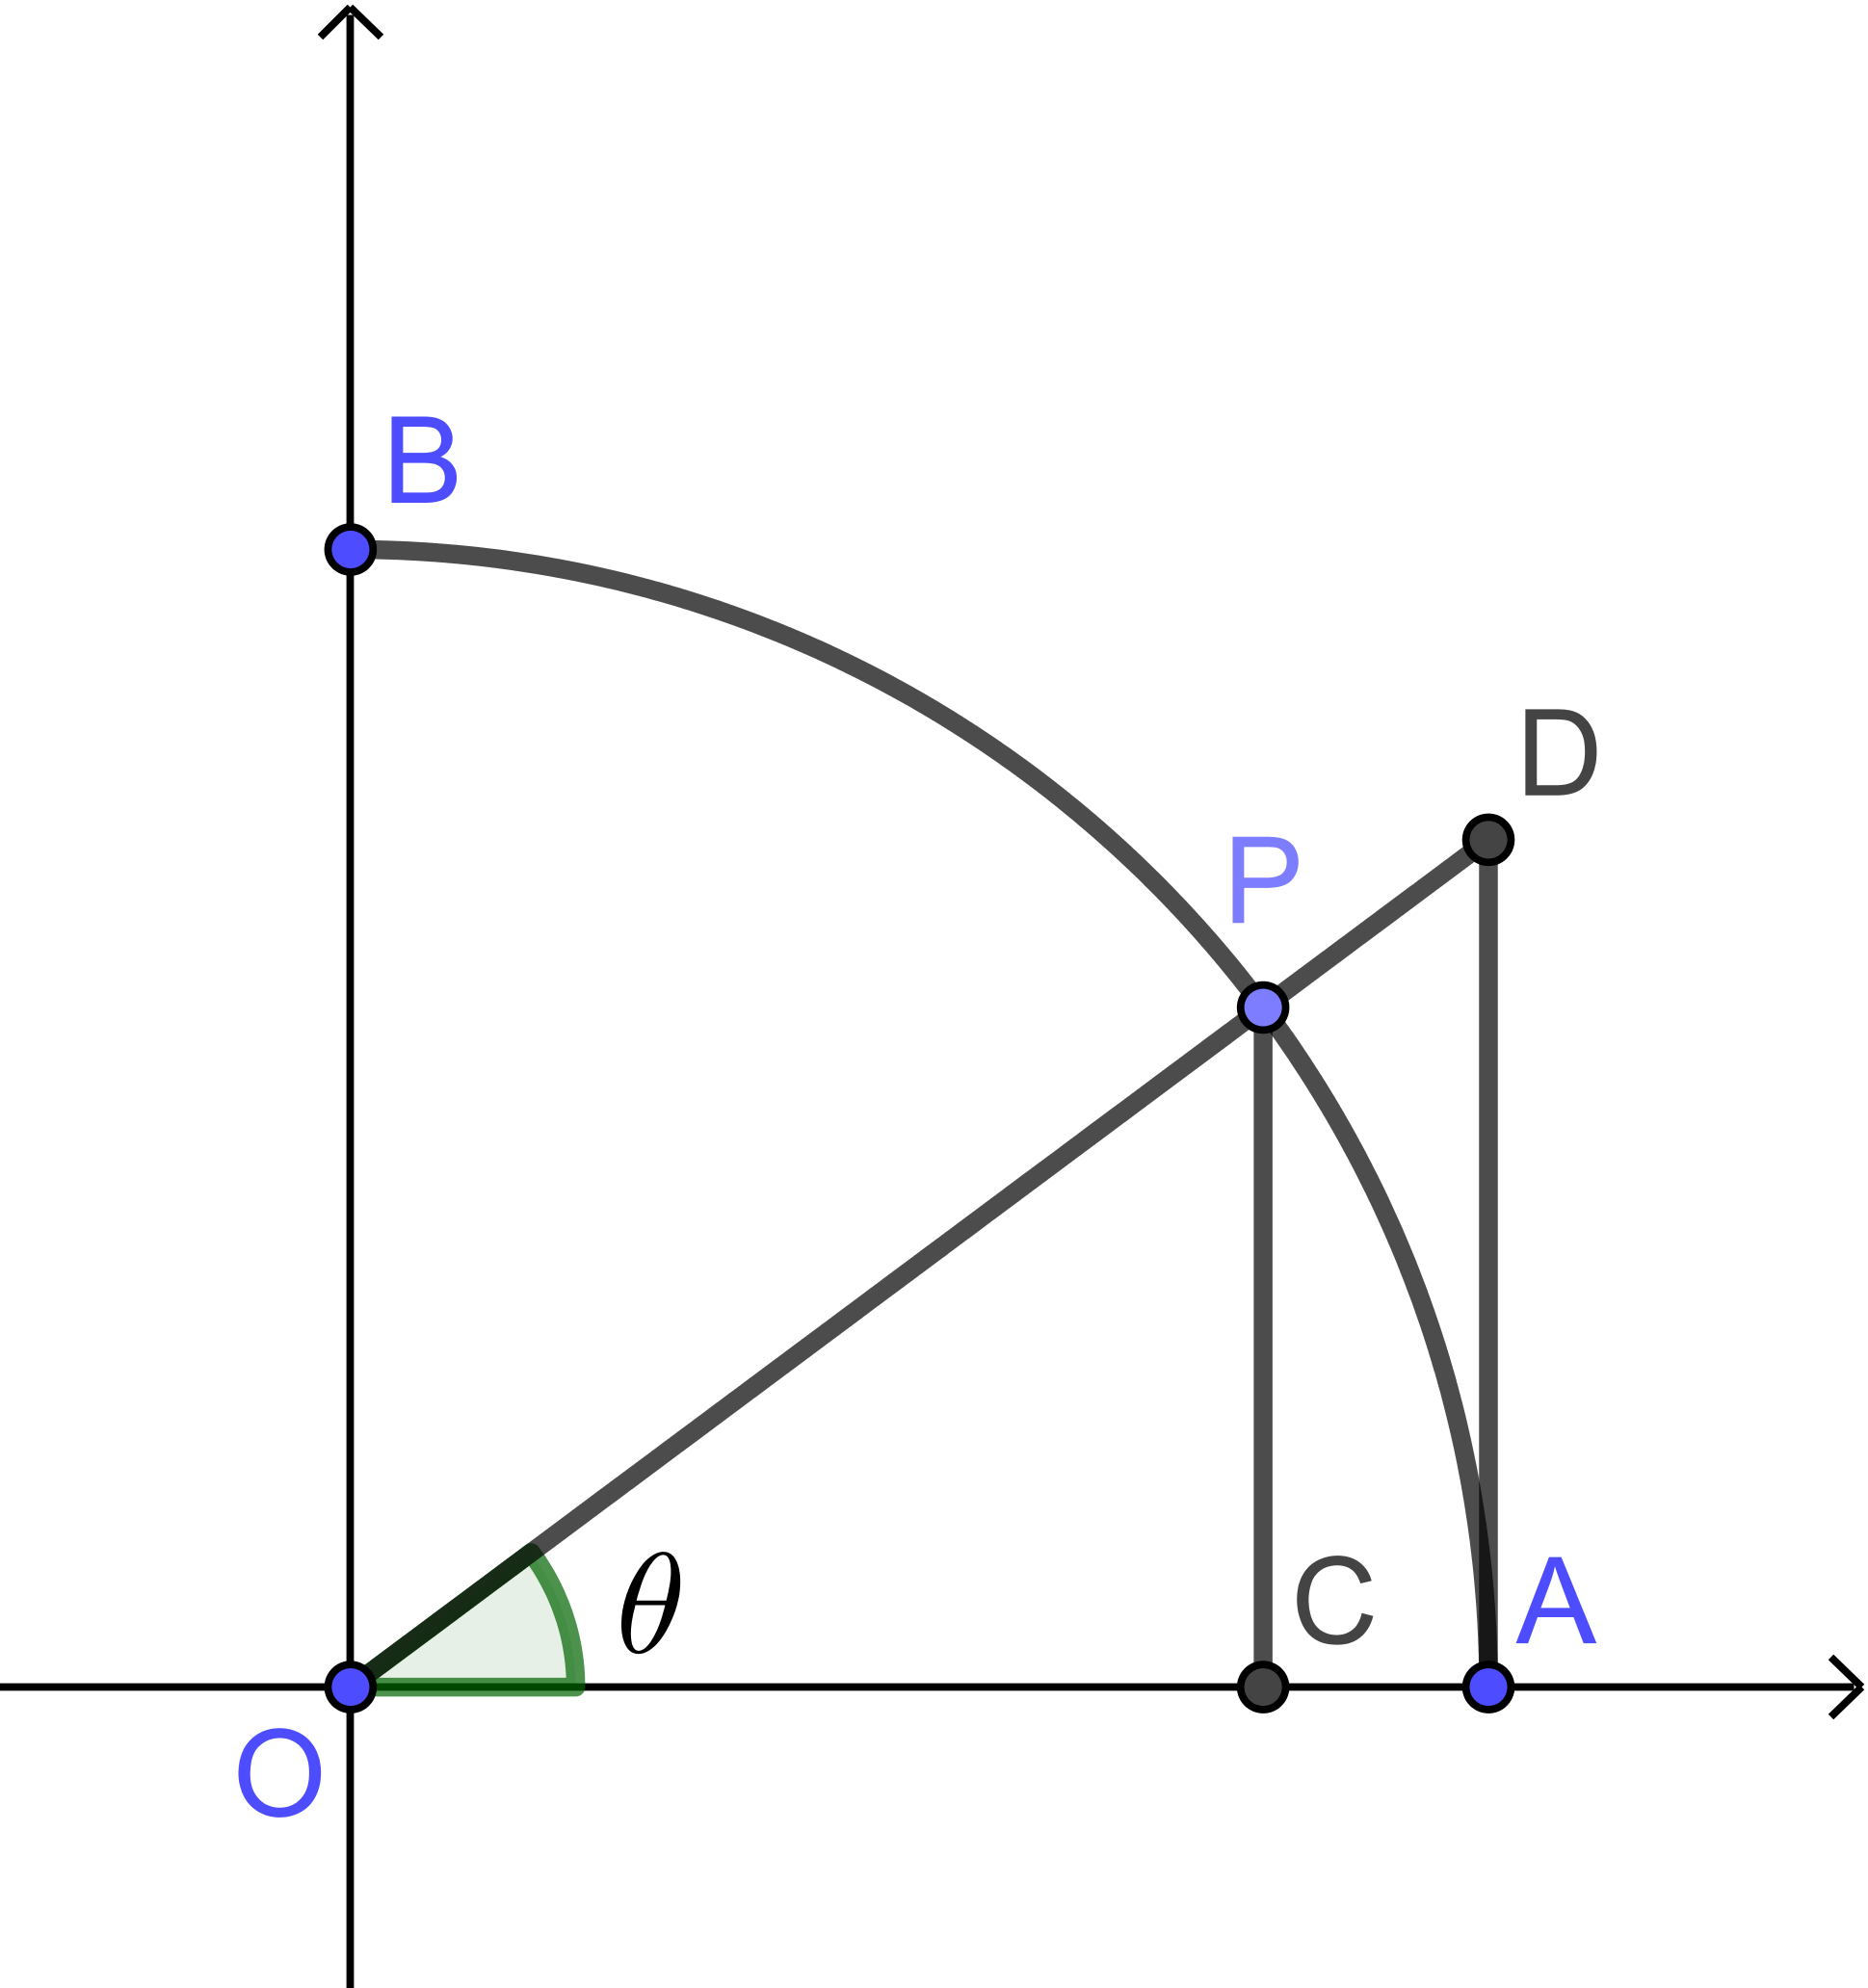
\includegraphics[width=.7\textwidth]{tratio_5}
\end{minipage}
\[
\sin\theta=\frac{\fbox{(가)}}{\ov OP}=\frac{\fbox{(나)}}{\ov OD}
\qquad
\cos\theta=\frac{\fbox{(다)}}{\ov OP}=\frac{\ov OA}{\ov OD}
\qquad
\tan\theta=\frac{\fbox{(가)}}{\fbox{(다)}}=\frac{\fbox{(나)}}{\ov OA}
\]
따라서
\[
\sin\theta=\fbox{(가)}
\qquad
\cos\theta=\fbox{(다)}
\qquad
\tan\theta=\fbox{(나)}
\]
\begin{enumerate}
\item
\(\theta=0\)의 삼각비를 구하려면 \(P=A\)인 상황을 생각하면 된다.
그러므로
\begin{center}
\begin{tabu}to.6\textwidth{X[$]X[$]X[$]}
\sin0=&\cos0=&\tan0=
\end{tabu}
\end{center}
\item
\(\theta=\frac\pi2\)의 삼각비를 구하려면 \(P=B\)인 상황을 생각하면 된다.
그러므로
\begin{center}
\begin{tabu}to.6\textwidth{X[$]X[$]X[$]}
\sin\frac\pi2=&\cos\frac\pi2=&\tan\frac\pi2=
\end{tabu}
\end{center}
\end{enumerate}

%%%
\section{삼각함수}
\begin{mdframed}
%
\defi{삼각함수의 값}\label{tfunction1}
\noindent\begin{minipage}{.75\textwidth}
양수 \(r\)에 대하여 점 \(A=(r,0)\)을 원 \(x^2+y^2=r^2\)을 따라 시계 반대 방향\footnotemark으로 \(\theta\)만큼 회전시킨 점을 \(P(x,y)\)라고 할 때,
\[\sin\theta=\frac yr,\quad\cos\theta=\frac xr,\quad\tan\theta=\frac yx\]
\end{minipage}
\begin{minipage}{.25\textwidth}
\centering
\vspace{10pt}
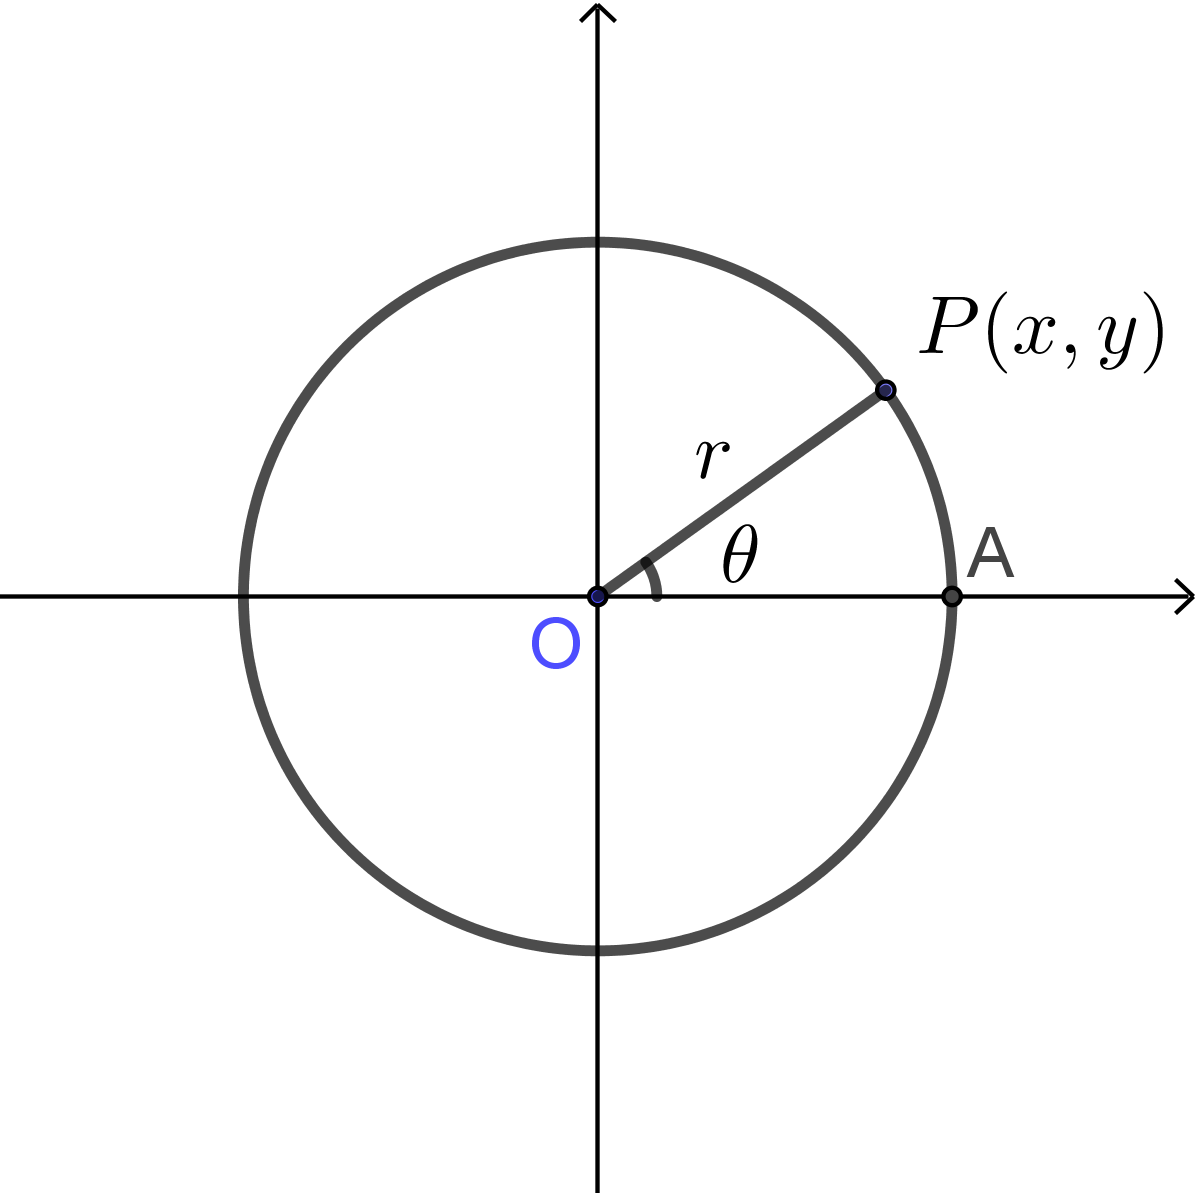
\includegraphics[width=.9\textwidth]{tfunction_1}
\vspace{10pt}
\end{minipage}
이다.
이때, 반직선 \(OA\)를 시초선, 반직선 \(OP\)를 동경이라고 부른다.
\end{mdframed}
\footnotetext{
시계 반대 방향은 시계 바늘이 도는 방향의 반대방향을 의미한다.
\(\theta<0\)이면 시계 방향으로 회전시킨다.
따라서 시계 반대 방향을 \fbox{양의 방향}, 시계 방향을 \fbox{음의 방향}이라고 부른다.}

%
\exam{\(\frac\pi6\), \(\frac34\pi\), \(\frac32\pi\), \(-\frac\pi6\)의 사인, 코사인, 탄젠트의 값을 각각 구하여라.}
\begin{enumerate}\label{tfunction2}
\item
\(r=2\)로 두고 \(A(2,0)\)를 시계반대방향으로 \(\frac\pi6(=30\textdegree{})\)만큼 회전시키면 \(P=(\sqrt3,1)\)이다.
따라서
\vspace{-10pt}
\par\noindent
\begin{minipage}{.5\textwidth}
\begin{talign*}
\sin\frac\pi6&=\frac12\\
\cos\frac\pi6&=\frac{\sqrt3}2\\
\tan\frac\pi6&=\frac1{\sqrt3}=\frac{\sqrt3}3
\end{talign*}
\end{minipage}
\begin{minipage}{.5\textwidth}
\vspace{10pt}
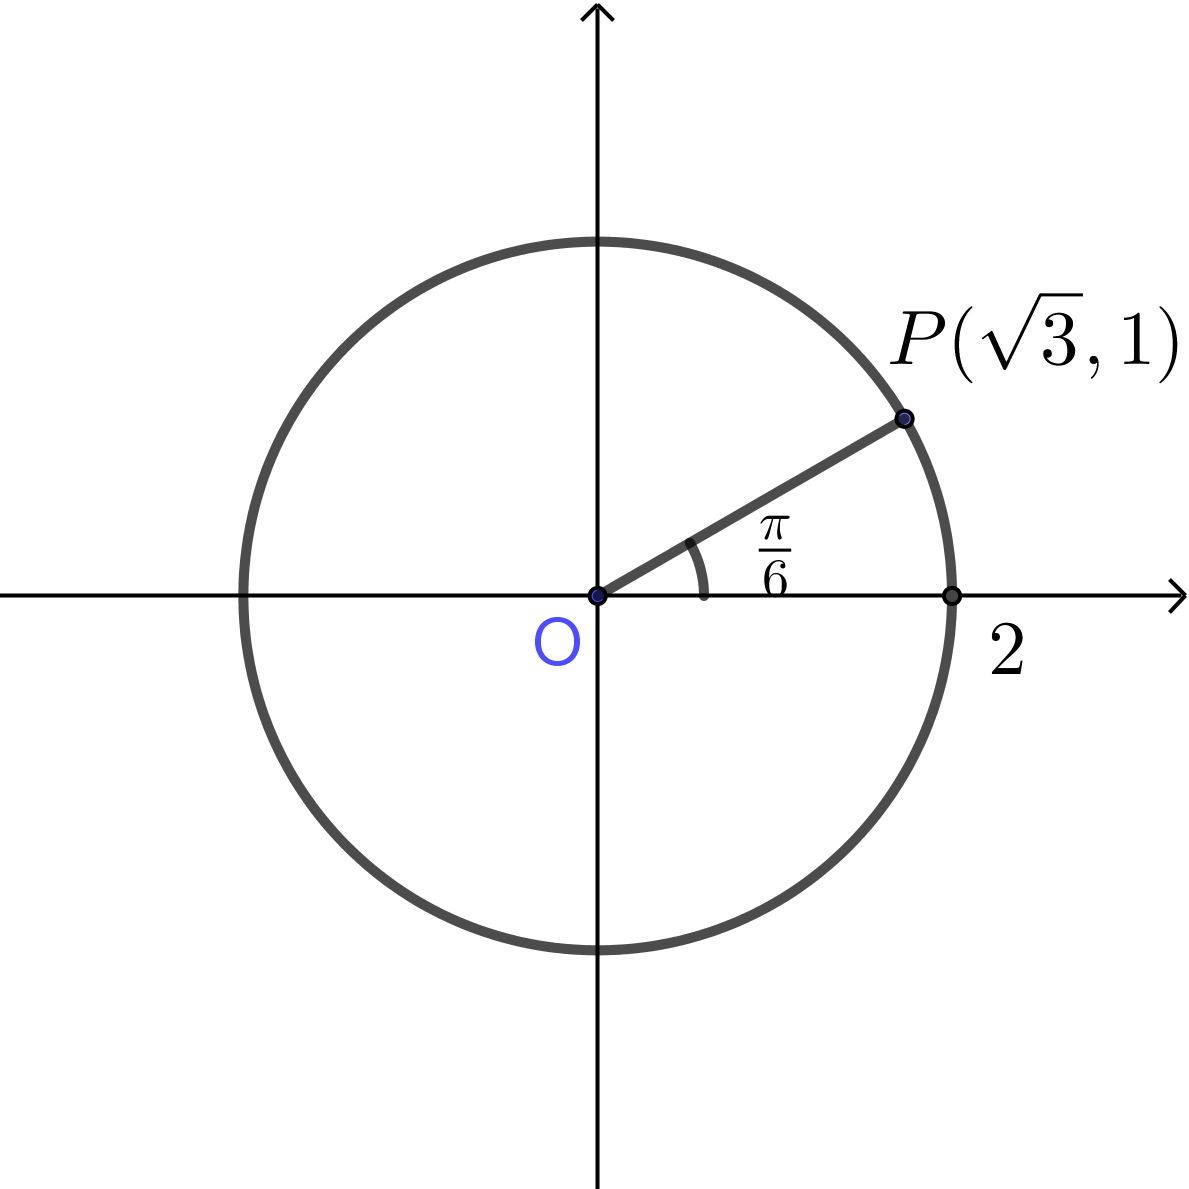
\includegraphics[width=.5\textwidth]{tfunction_2-1}
\vspace{10pt}
\end{minipage}
%\[\sin \frac\pi6=\frac12,\quad\cos \frac\pi6=\frac{\sqrt3}2,\quad\tan \frac\pi6=\frac1{\sqrt3}=\frac{\sqrt3}3\]
\item
\(r=\sqrt2\)로 두고 \(A(\sqrt2,0)\)를 시계반대방향으로 \(\frac34\pi(=135\textdegree{})\)만큼 회전시키면 \(P=(-1,\sqrt2)\)이다.
따라서
\par\noindent
\begin{minipage}{.5\textwidth}
\begin{talign*}
\sin\frac34\pi&=\frac1{\sqrt2}=\frac{\sqrt2}2\\
\cos\frac34\pi&=\frac{-1}{\sqrt2}=-\frac{\sqrt2}2\\
\tan\frac34\pi&=\frac1{-1}=-1
\end{talign*}
\end{minipage}
\begin{minipage}{.5\textwidth}
\vspace{10pt}
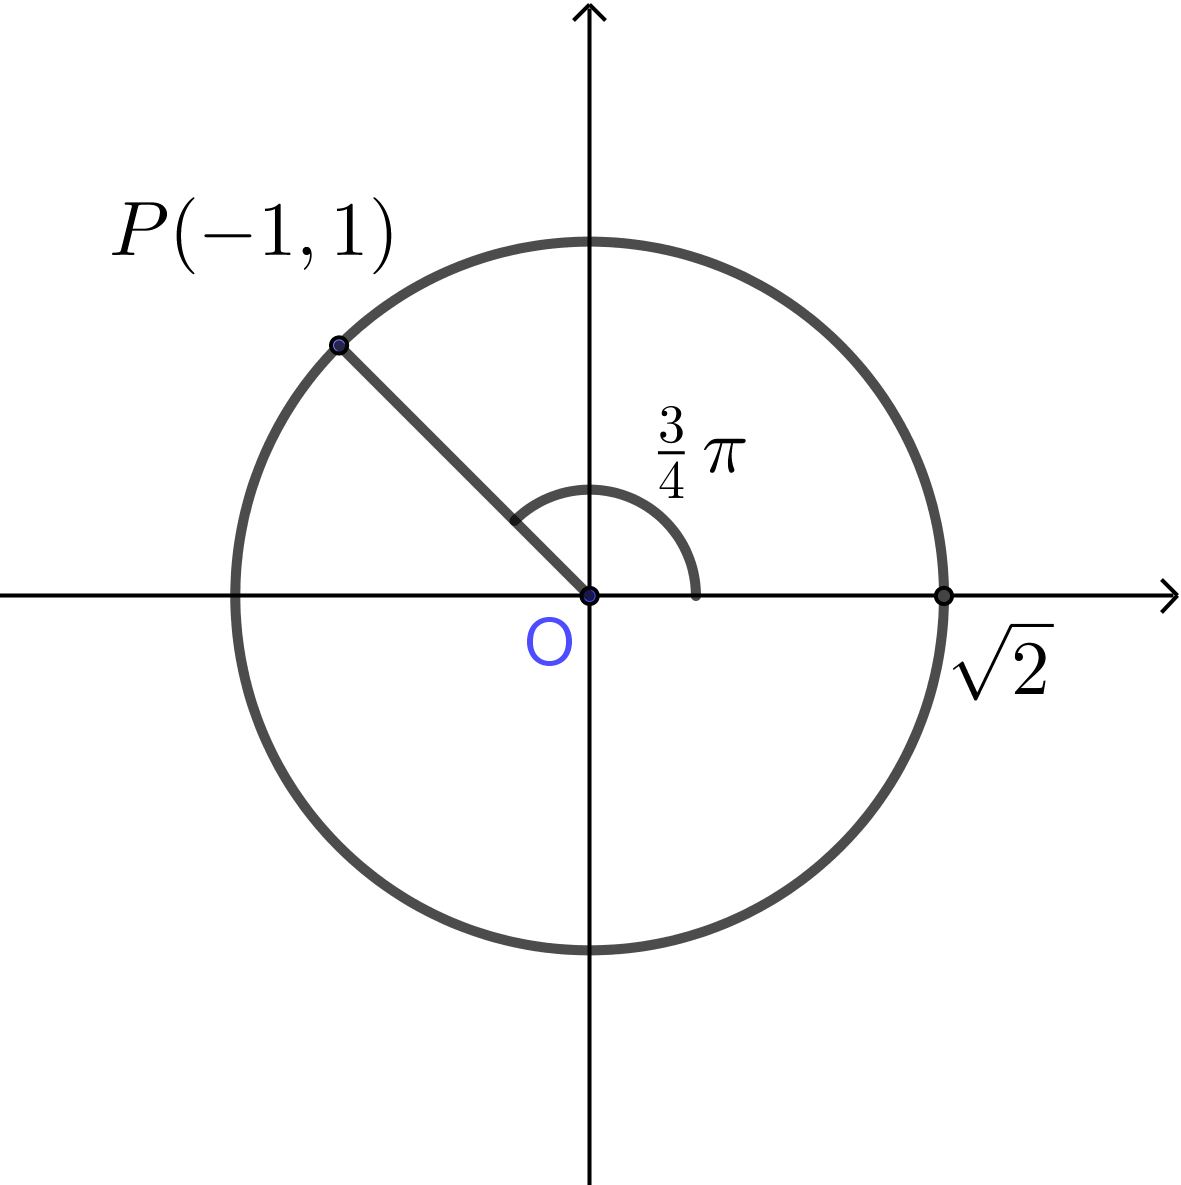
\includegraphics[width=.5\textwidth]{tfunction_2-2}
\vspace{10pt}
\end{minipage}
%\[\sin \frac34\pi=\frac1{\sqrt2}=\frac{\sqrt2}2,\quad\cos \frac34\pi=\frac1{-1}=-1,\quad\tan\frac34\pi=\frac{-1}{\sqrt2}=-\frac{\sqrt2}2\]
\newpage
\item
\(r=1\)로 두고 \(A(1,0)\)를 시계반대방향으로 \(\frac32\pi(=270\textdegree{})\)만큼 회전시키면 \(P=(0,-1)\)이다.
따라서
\par\noindent
\begin{minipage}{.5\textwidth}
\begin{talign*}
\sin\frac32\pi&=\frac01=0\\
\cos\frac32\pi&=\frac{-1}1=-1\\
\tan\frac32\pi&=\frac{-1}0\text{\scriptsize(존재하지 않는다.)}
\end{talign*}
\end{minipage}
\begin{minipage}{.5\textwidth}
\vspace{10pt}
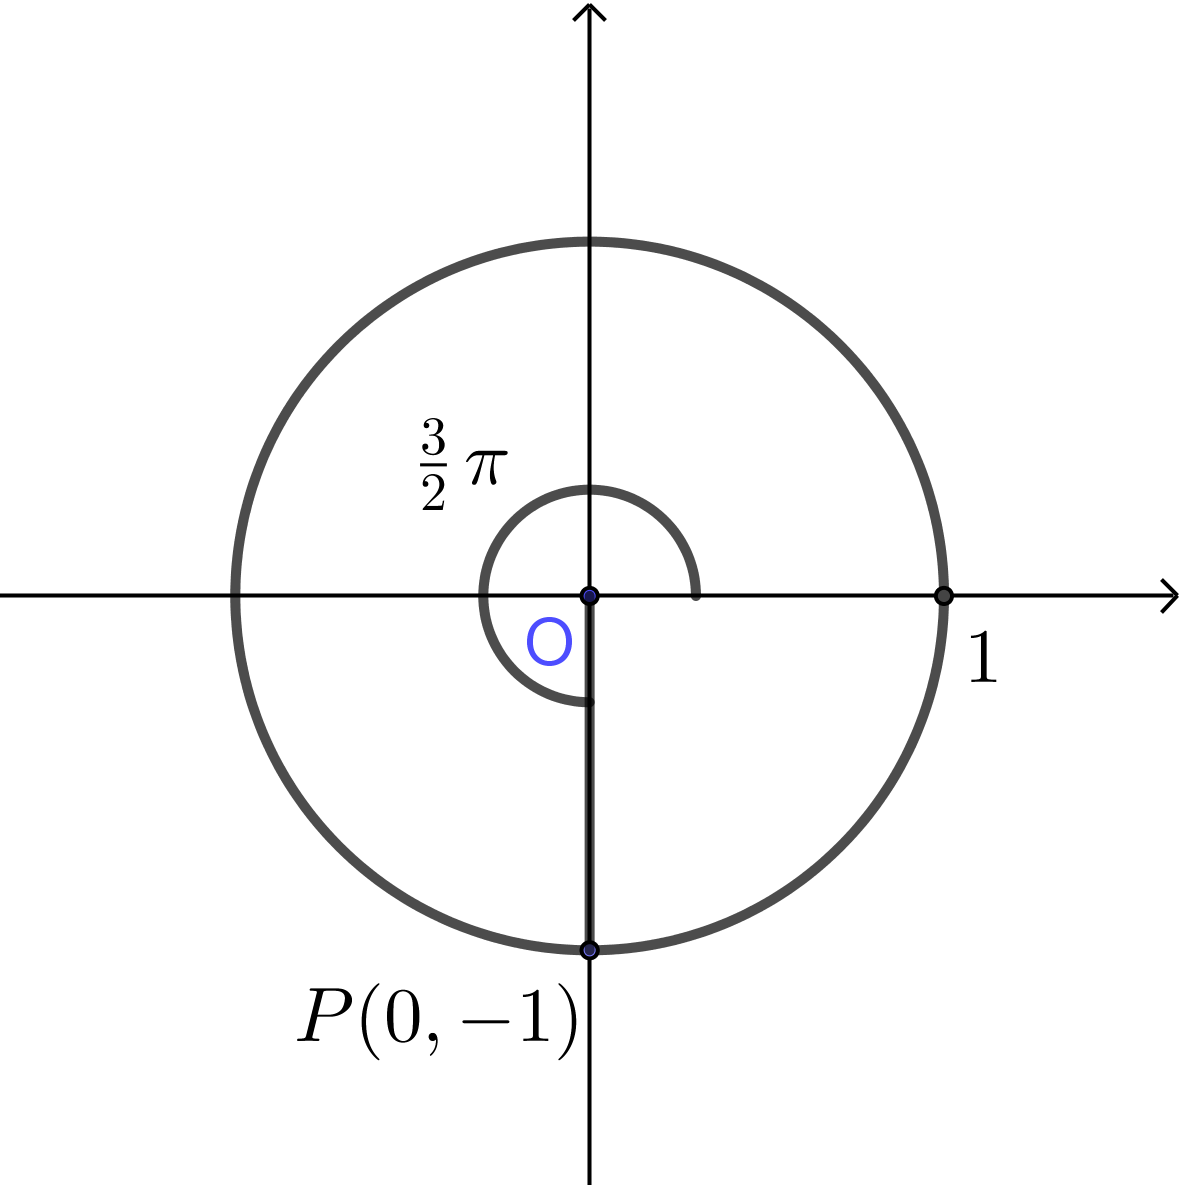
\includegraphics[width=.5\textwidth]{tfunction_2-3}
\vspace{10pt}
\end{minipage}
\item
\(r=2\)로 두고 \(A(2,0)\)를 시계방향으로 \(\frac\pi6(=30\textdegree{})\)만큼 회전시키면\\ \(P=(\sqrt3,-1)\)이다.
따라서
\par\noindent
\begin{minipage}{.5\textwidth}
\begin{talign*}
\sin\left(-\frac\pi6\right)&=\frac{-1}2=-\frac12\\
\cos\left(-\frac\pi6\right)&=\frac{\sqrt3}2\\
\tan\left(-\frac\pi6\right)&=\frac{-1}{\sqrt3}=-\frac{\sqrt3}3
\end{talign*}
\end{minipage}
\begin{minipage}{.5\textwidth}
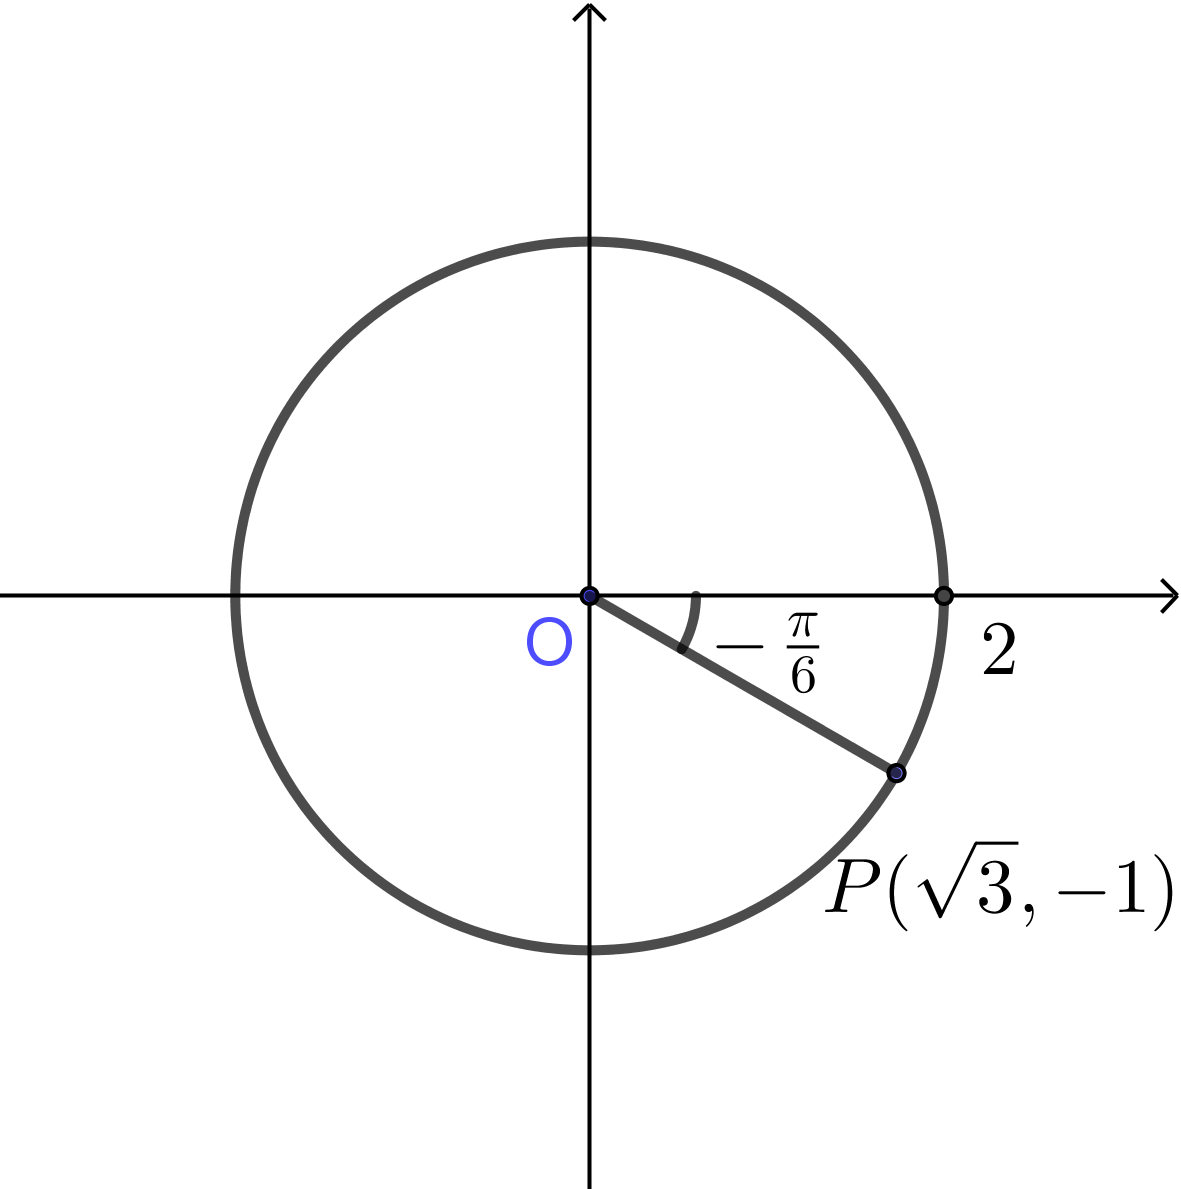
\includegraphics[width=.5\textwidth]{tfunction_2-4}
\end{minipage}
\end{enumerate}

%
\prob{\(\frac\pi4\), \(\frac23\pi\), \(\frac73\pi\), \(-\pi\)의 사인, 코사인, 탄젠트의 값을 각각 구하여라.}\label{tfunction3}
\par\noindent
\begin{minipage}{.25\textwidth}
\begin{talign*}
\sin\frac\pi4&=\\
\cos\frac\pi4&=\\\
\tan\frac\pi4&=
\end{talign*}
\end{minipage}
\begin{minipage}{.25\textwidth}
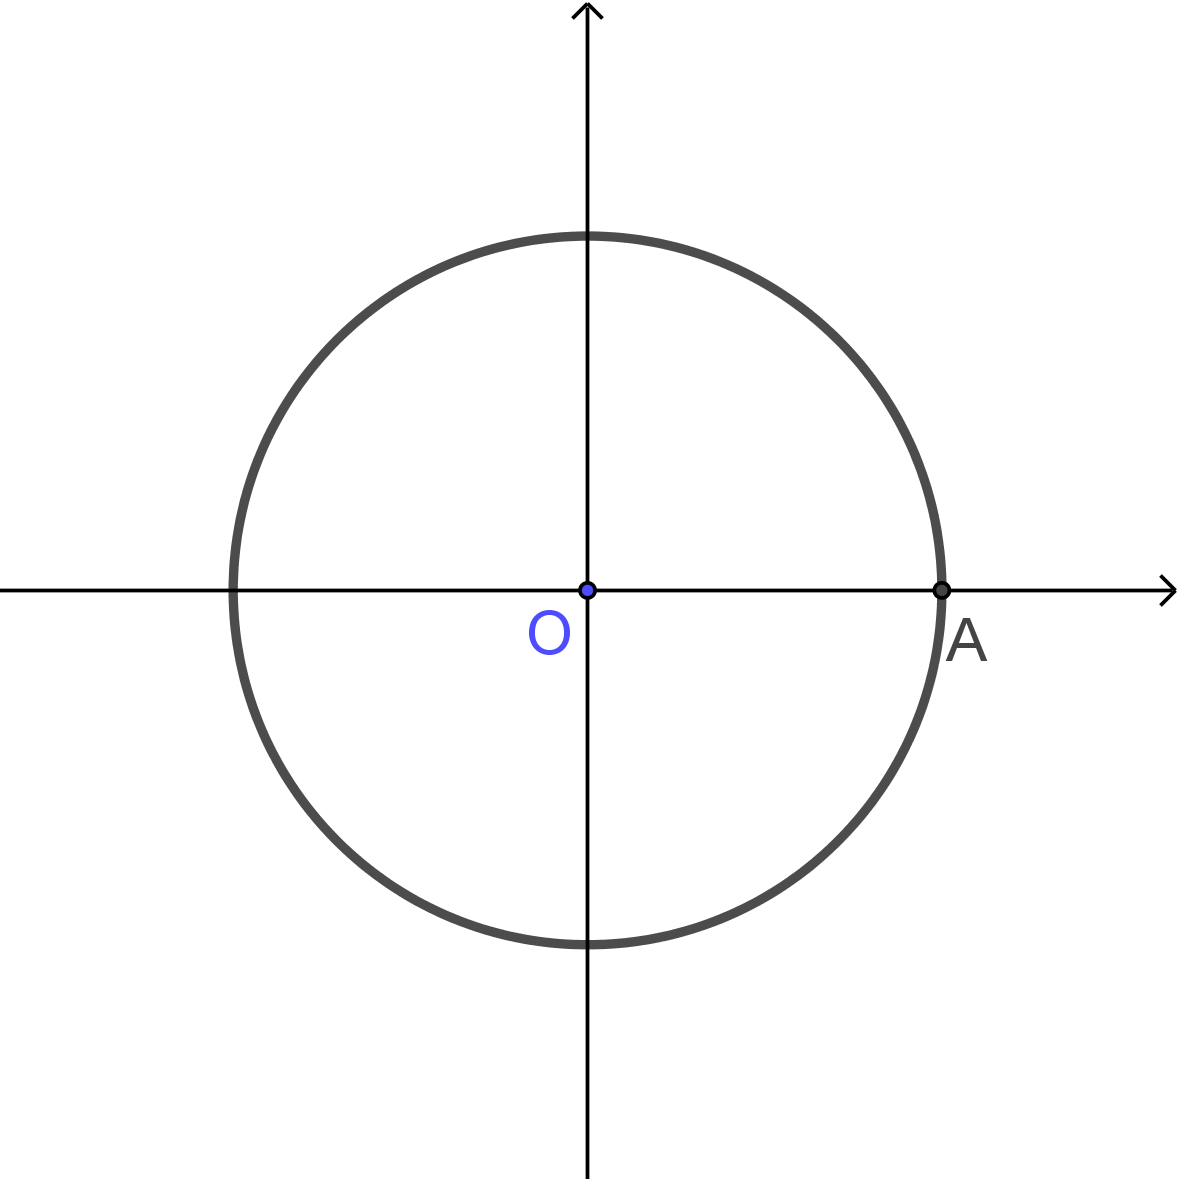
\includegraphics[width=\textwidth]{tfunction_3}
\end{minipage}
\begin{minipage}{.25\textwidth}
\begin{talign*}
\sin\frac23\pi&=\\
\cos\frac23\pi&=\\\
\tan\frac23\pi&=
\end{talign*}
\end{minipage}
\begin{minipage}{.25\textwidth}
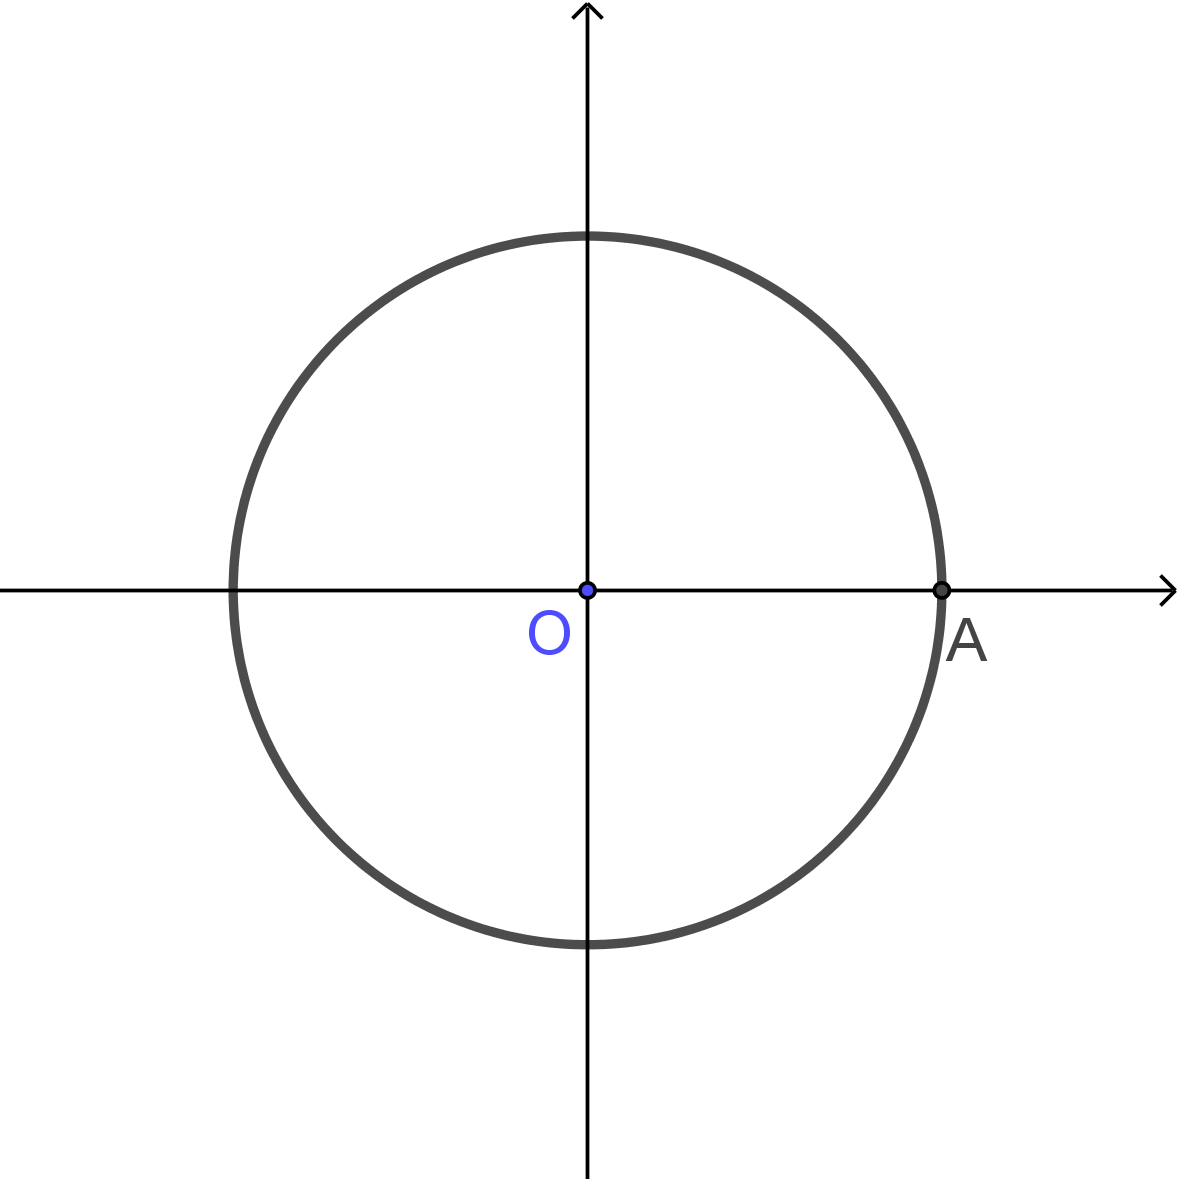
\includegraphics[width=\textwidth]{tfunction_3}
\end{minipage}
%
\bigskip\par\noindent
\begin{minipage}{.25\textwidth}
\begin{talign*}
\sin\frac73\pi&=\\
\cos\frac73\pi&=\\\
\tan\frac73\pi&=
\end{talign*}
\end{minipage}
\begin{minipage}{.25\textwidth}
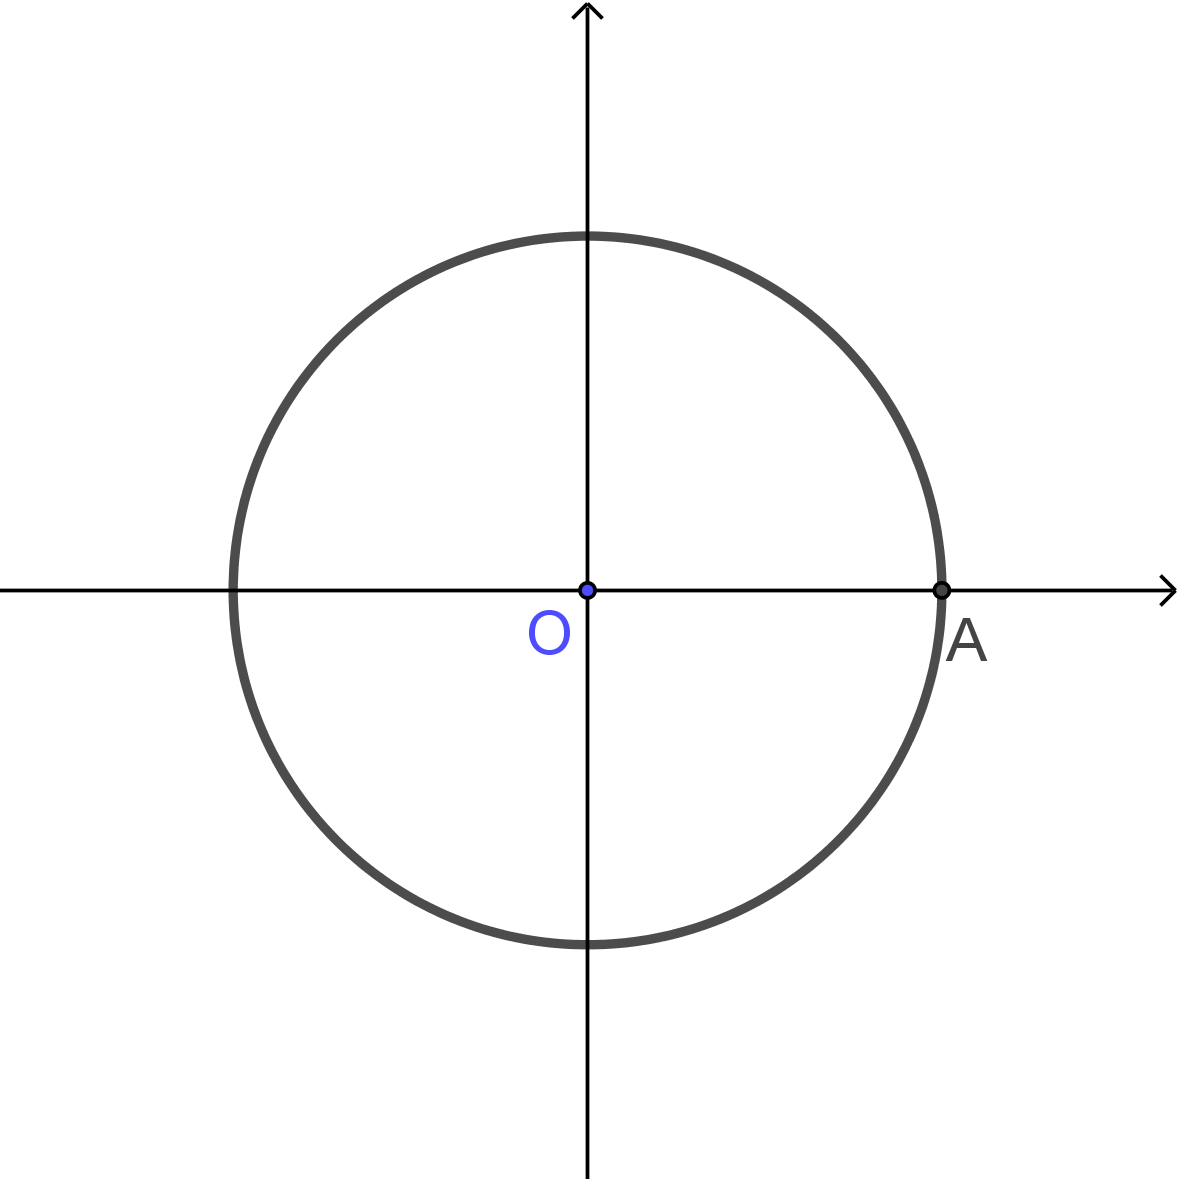
\includegraphics[width=\textwidth]{tfunction_3}
\end{minipage}
\begin{minipage}{.25\textwidth}
\begin{talign*}
\sin(-\pi)&=\\
\cos(-\pi)&=\\\
\tan(-\pi)&=
\end{talign*}
\end{minipage}
\begin{minipage}{.25\textwidth}
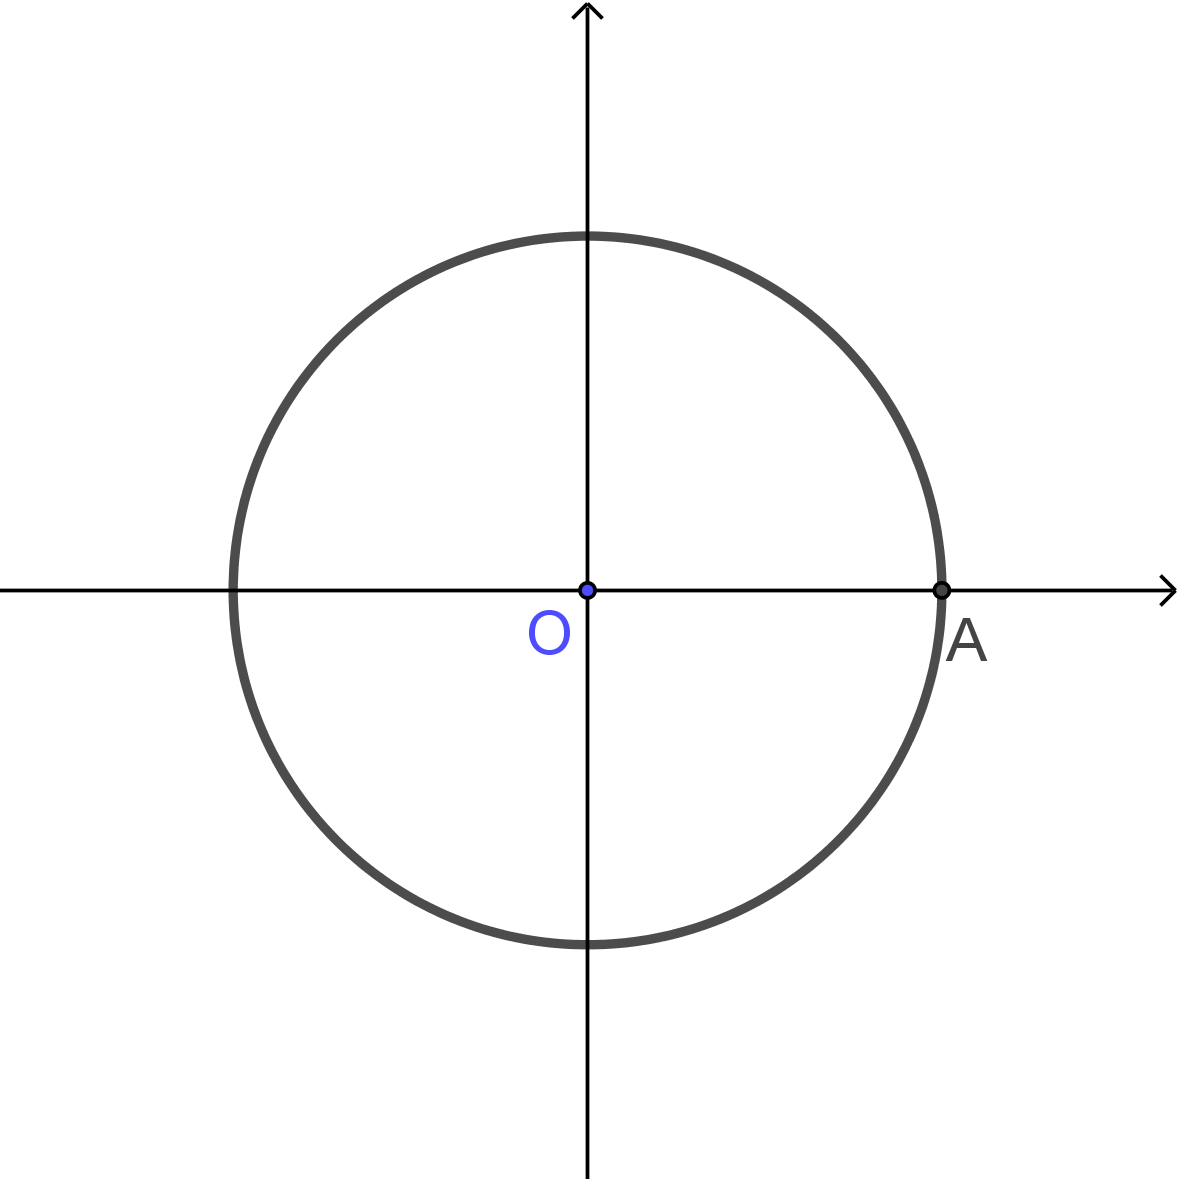
\includegraphics[width=\textwidth]{tfunction_3}
\end{minipage}

%%%
\section{삼각함수의 성질}
%\noindent\begin{minipage}{.7\textwidth}
%원 \(x^2+y^2=r^2\) 위의 점 \(P(x,y)\)에 대하여
%\[\sin\theta=\frac yr,\quad\cos\theta=\frac xr,\quad\tan\theta=\frac yx\]
%이었다.
%%이때, \(|x|\le r\)이므로 \(-1\le\sin\theta\le1\)이다.
%%마찬가지로 \(-1\le\cos\theta\le1\)도 성립한다.
%따라서
%\end{minipage}
%\begin{minipage}{.3\textwidth}
%\centering
%\vspace{10pt}
%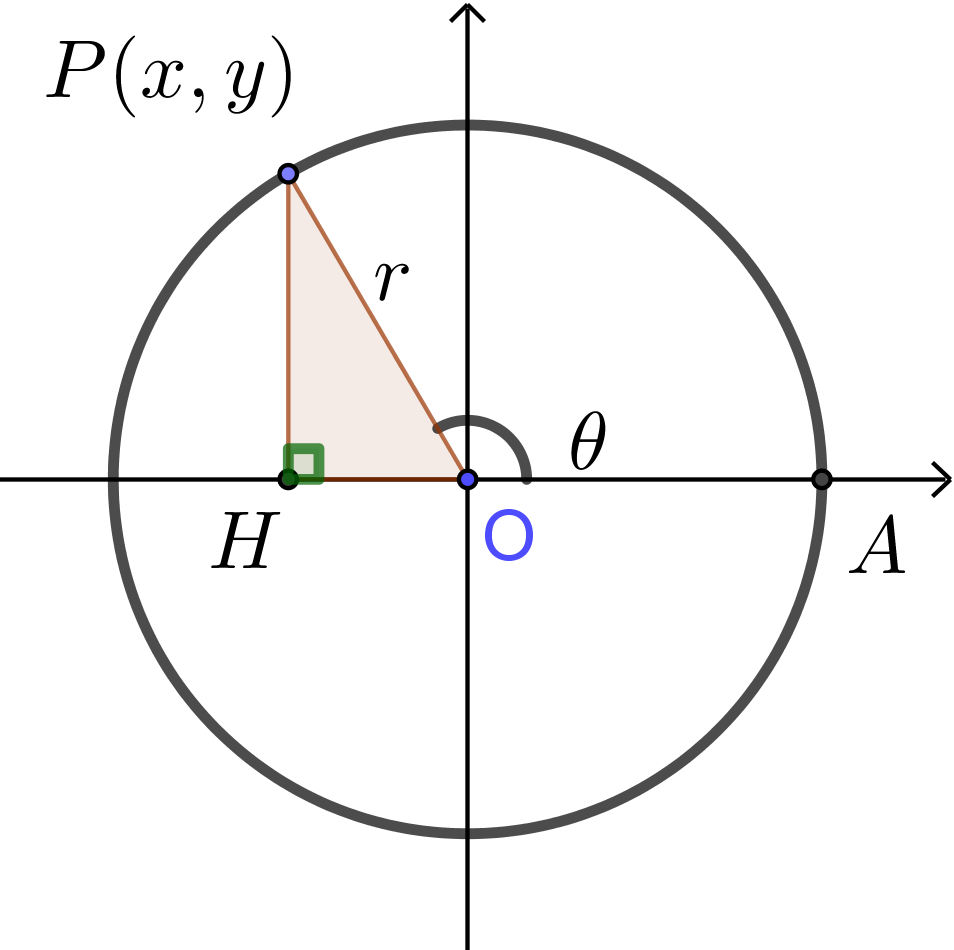
\includegraphics[width=\textwidth]{property_1}
%\vspace{10pt}
%\end{minipage}
%\[\frac{\sin\theta}{\cos\theta}=\frac{y/r}{x/r}=\frac yx=\tan\theta\]
%이다.
%한편, \(\ov OH=|x|\), \(\ov PH=|y|\)이므로, 삼각형 \(OHP\)에 피타고라스의 정리를 쓰면 
%\(x^2+y^2=r^2\)이다.
%양변을 \(r^2\)으로 나누면 \((\frac xr)^2+(\frac yr)^2=1\)이다.
%즉
%\[\sin^2\theta+\cos^2\theta=1\]
%이다.%
%\footnote{\((\sin\theta)^2\)은 \(\sin^2\theta\)로 표기한다.}

\noindent\begin{minipage}{.7\textwidth}
오른쪽 그림에서 %삼각형 \(OHP\)는 \ov OP를 빗변으로 하는 직각삼각형이다.
%\(\ov OP=r\), \(\ov OH=|x|\), \(\ov PH=|y|\)이고 \(|x|\le r\), \(|y|\le r\)이므로
\(-r\le x\le r\), \(-r\le y\le r\)
이다.\\
두 식의 양변을 \(r\)로 나누면
\[-1\le\cos\theta\le1,\quad-1\le\sin\theta\le1\]
이다.
또한, 식 \(x^2+y^2=r^2\)에서 양변을 \(r^2\)으로\\
나누어주면\footnotemark
\end{minipage}
\begin{minipage}{.3\textwidth}
\centering
\vspace{10pt}
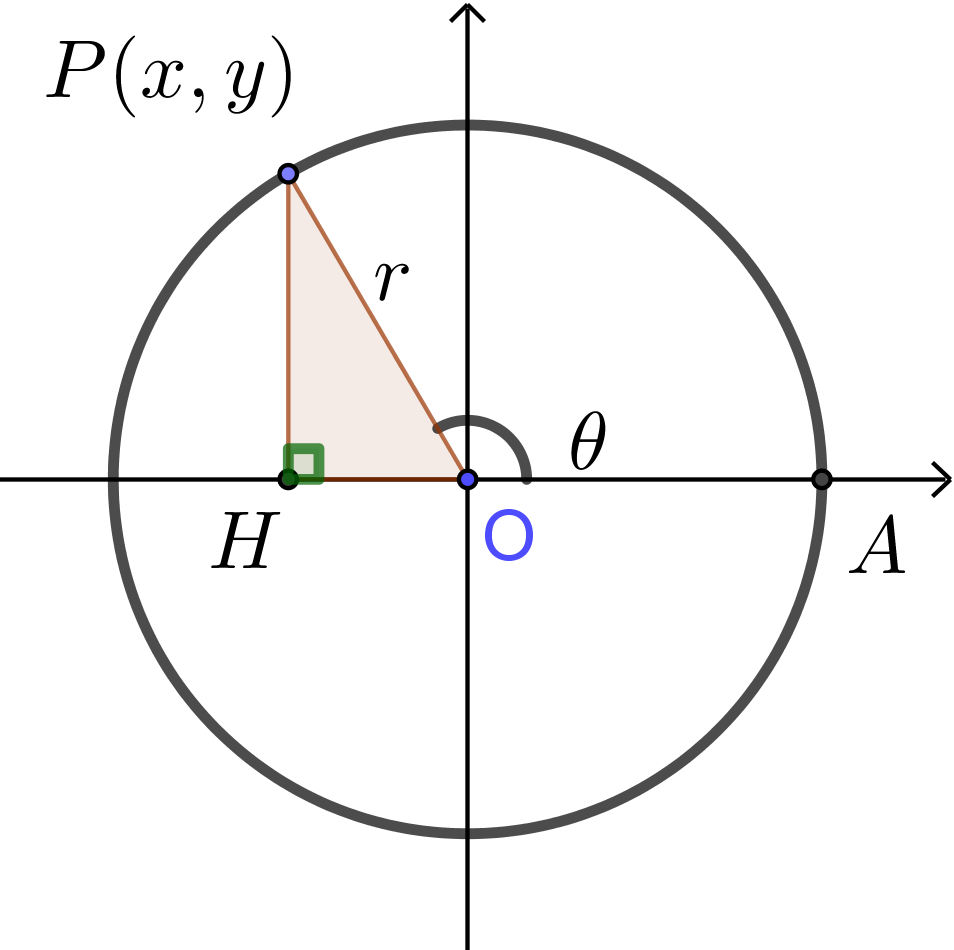
\includegraphics[width=.8\textwidth]{property_1}
\vspace{10pt}
\end{minipage}
\footnotetext{\((\sin\theta)^2\)은 \(\sin^2\theta\)로 표기한다.}
\[\sin^2\theta+\cos^2\theta=1\]
이다.
한편,
\[\frac{\sin\theta}{\cos\theta}=\frac{y/r}{x/r}=\frac yx=\tan\theta\]
도 성립한다.

\bigskip
\begin{mdframed}
%
\defi{삼각함수의 기본 성질}
\begin{enumerate}\label{property1}
\item
\(-1\le\sin\theta\le1\), \(-1\le\cos\theta\le1\)
\item
\(\sin^2\theta+\cos^2\theta=1\)
\item
\(\tan\theta=\frac{\sin\theta}{\cos\theta}\)
\end{enumerate}
\end{mdframed}

%
\prob{}
\begin{enumerate}\label{property2}
\item
\(2\sin^2\theta+3\sin\theta-2=0\)일 때, \(\sin\theta\)의 값을 구하시오.
\item
\(\sin\theta=\frac{2\sqrt2}3\)일 때, \(\cos\theta\)의 값으로 가능한 것을 모두 구하시오.
\item
\(\sin\theta=\frac35\), \(\cos\theta=\frac45\)일 때, \(\tan\theta\)의 값을 구하시오.
\item
\(\sin\theta=\frac{\sqrt{21}}5\)이고, \(0\le\theta\le\frac\pi2\)일 때, \(\tan\theta\)의 값을 구하여라.
\end{enumerate}

\newpage
%
\exam{각도 \(\theta\)의 동경을 \(OP\)라고 할 때, \(P=(4,3)\)이다.}\label{property3}
\par\noindent
\begin{minipage}{.5\textwidth}
\begin{talign*}
\sin\theta&=\frac35\\
\cos\theta&=\frac45\\
\tan\theta&=\frac34
\end{talign*}
\end{minipage}
\begin{minipage}{.5\textwidth}
\vspace{10pt}
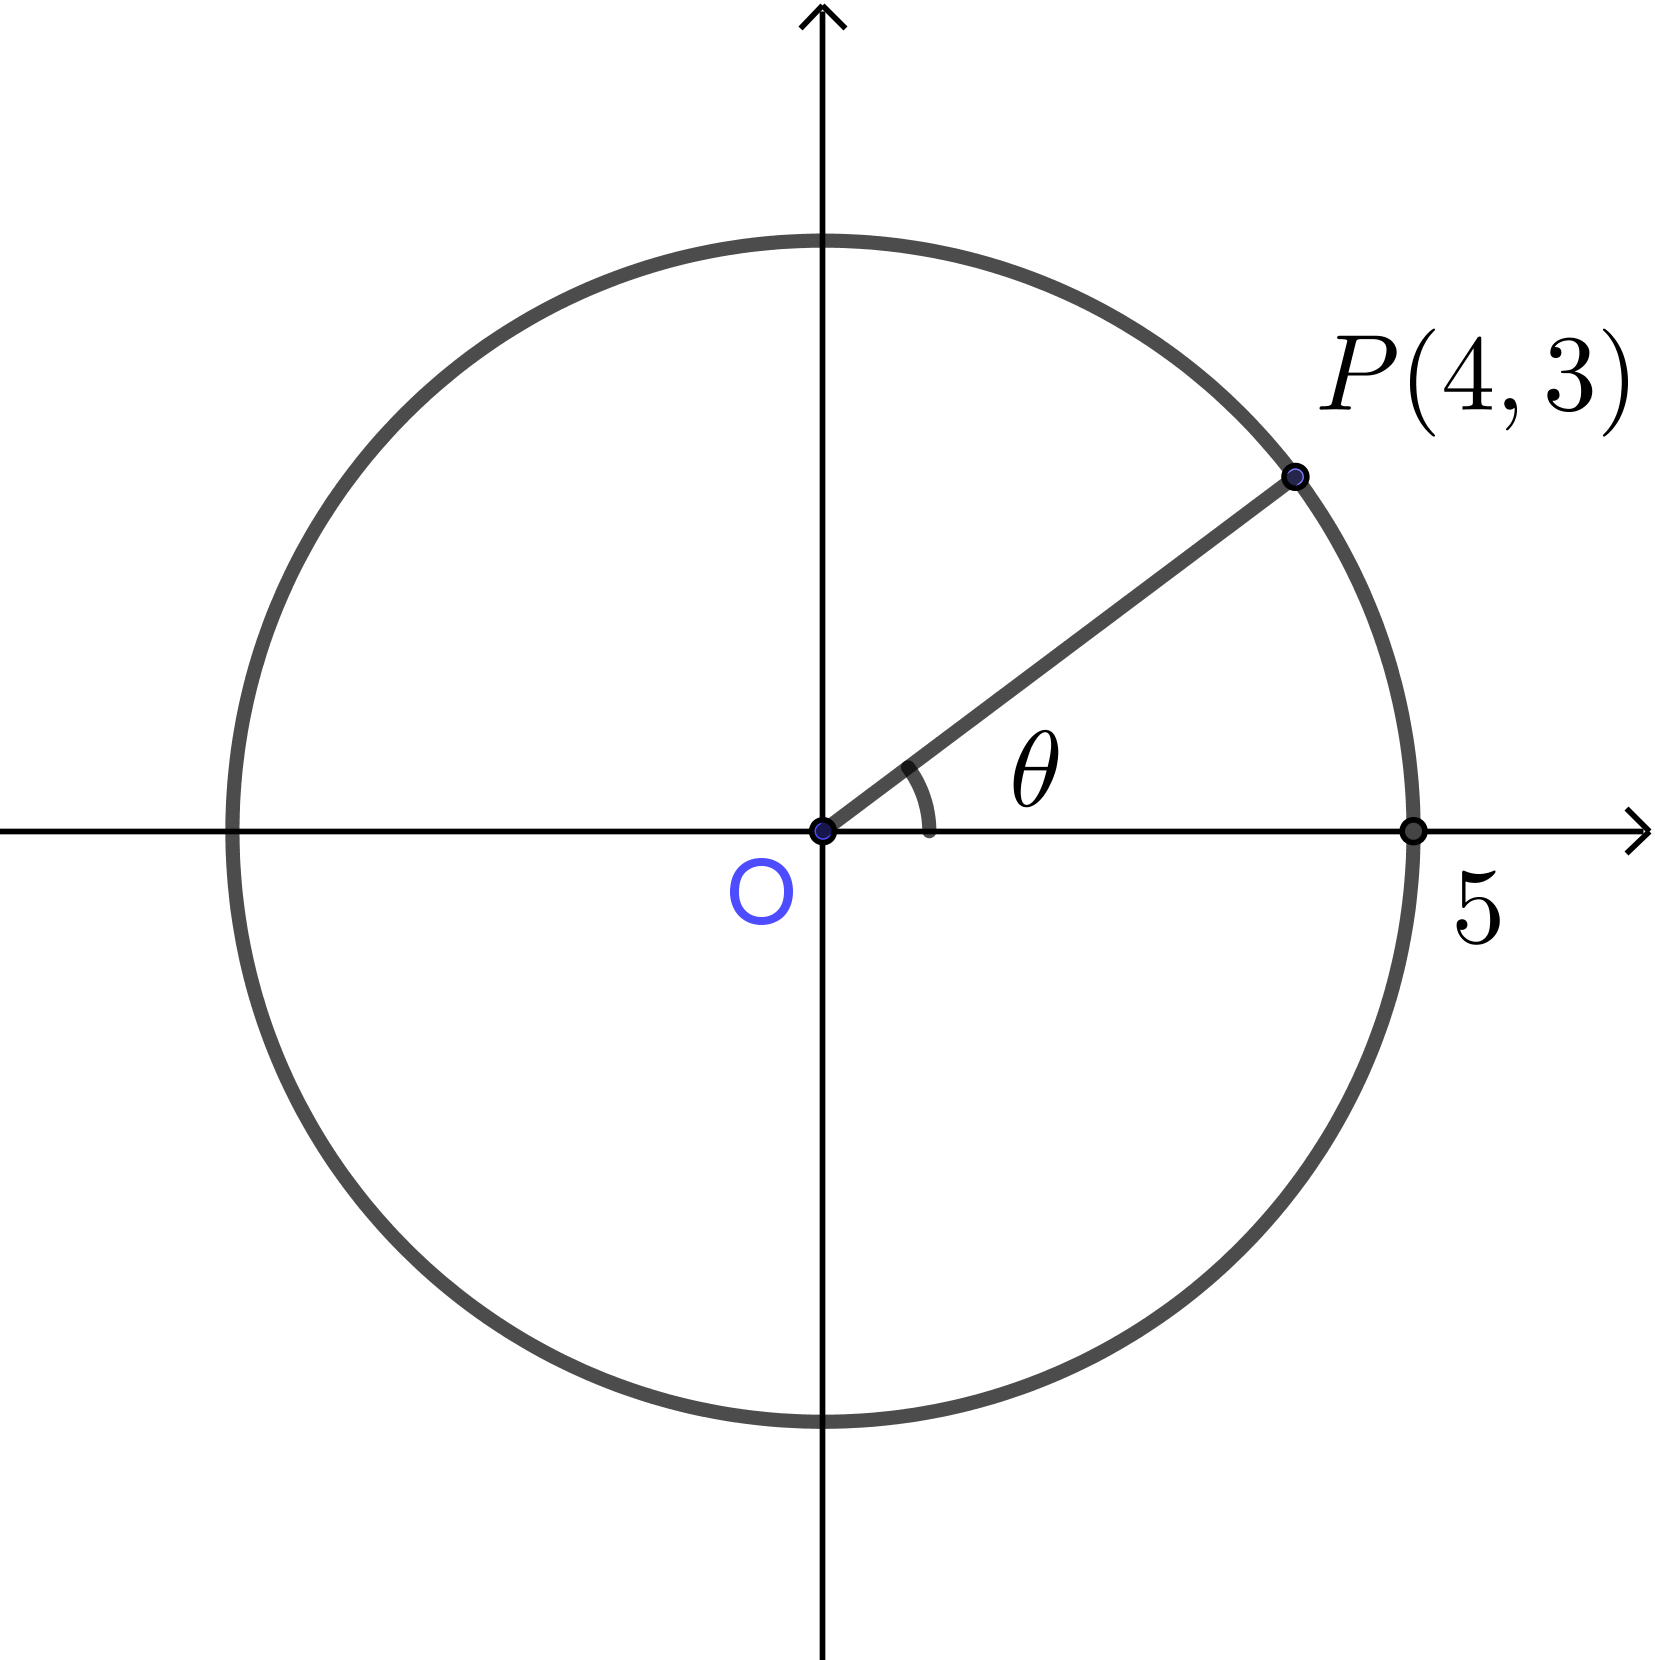
\includegraphics[width=.5\textwidth]{property_3}
\vspace{10pt}
\end{minipage}
\par\vspace{30pt}
\noindent
이때 다음 각도들에 대한 삼각비의 값을 차례로 구하여라.\\[10pt]
\begin{enumerate*}[itemjoin=\qquad\qquad]
\item
\(\theta+2\pi\)
\item
\(-\theta\)
\item
\(\theta+\pi\)
\item
\(\frac\pi2-\theta\)
\end{enumerate*}

\begin{mdframed}[nobreak=false]
\begin{enumerate}
\item
\(\theta+2\pi\)의 동경을 \(OP_1\)이라고 하면, \(P_1\)은 \(A\)를 \(\theta\)만큼 시계 반대 방향으로 회전시킨 후(\(=P\)) 같은 방향으로 \(2\pi\)만큼 더 회전시킨 점이다.
따라서 \(P_1=P=(4,3)\)이다.
\par\noindent
\begin{minipage}{.5\textwidth}
\begin{talign*}
\sin(\theta+2\pi)&=\frac35\\
\cos(\theta+2\pi)&=\frac45\\
\tan(\theta+2\pi)&=\frac34
\end{talign*}
\end{minipage}
\begin{minipage}{.5\textwidth}
\vspace{10pt}
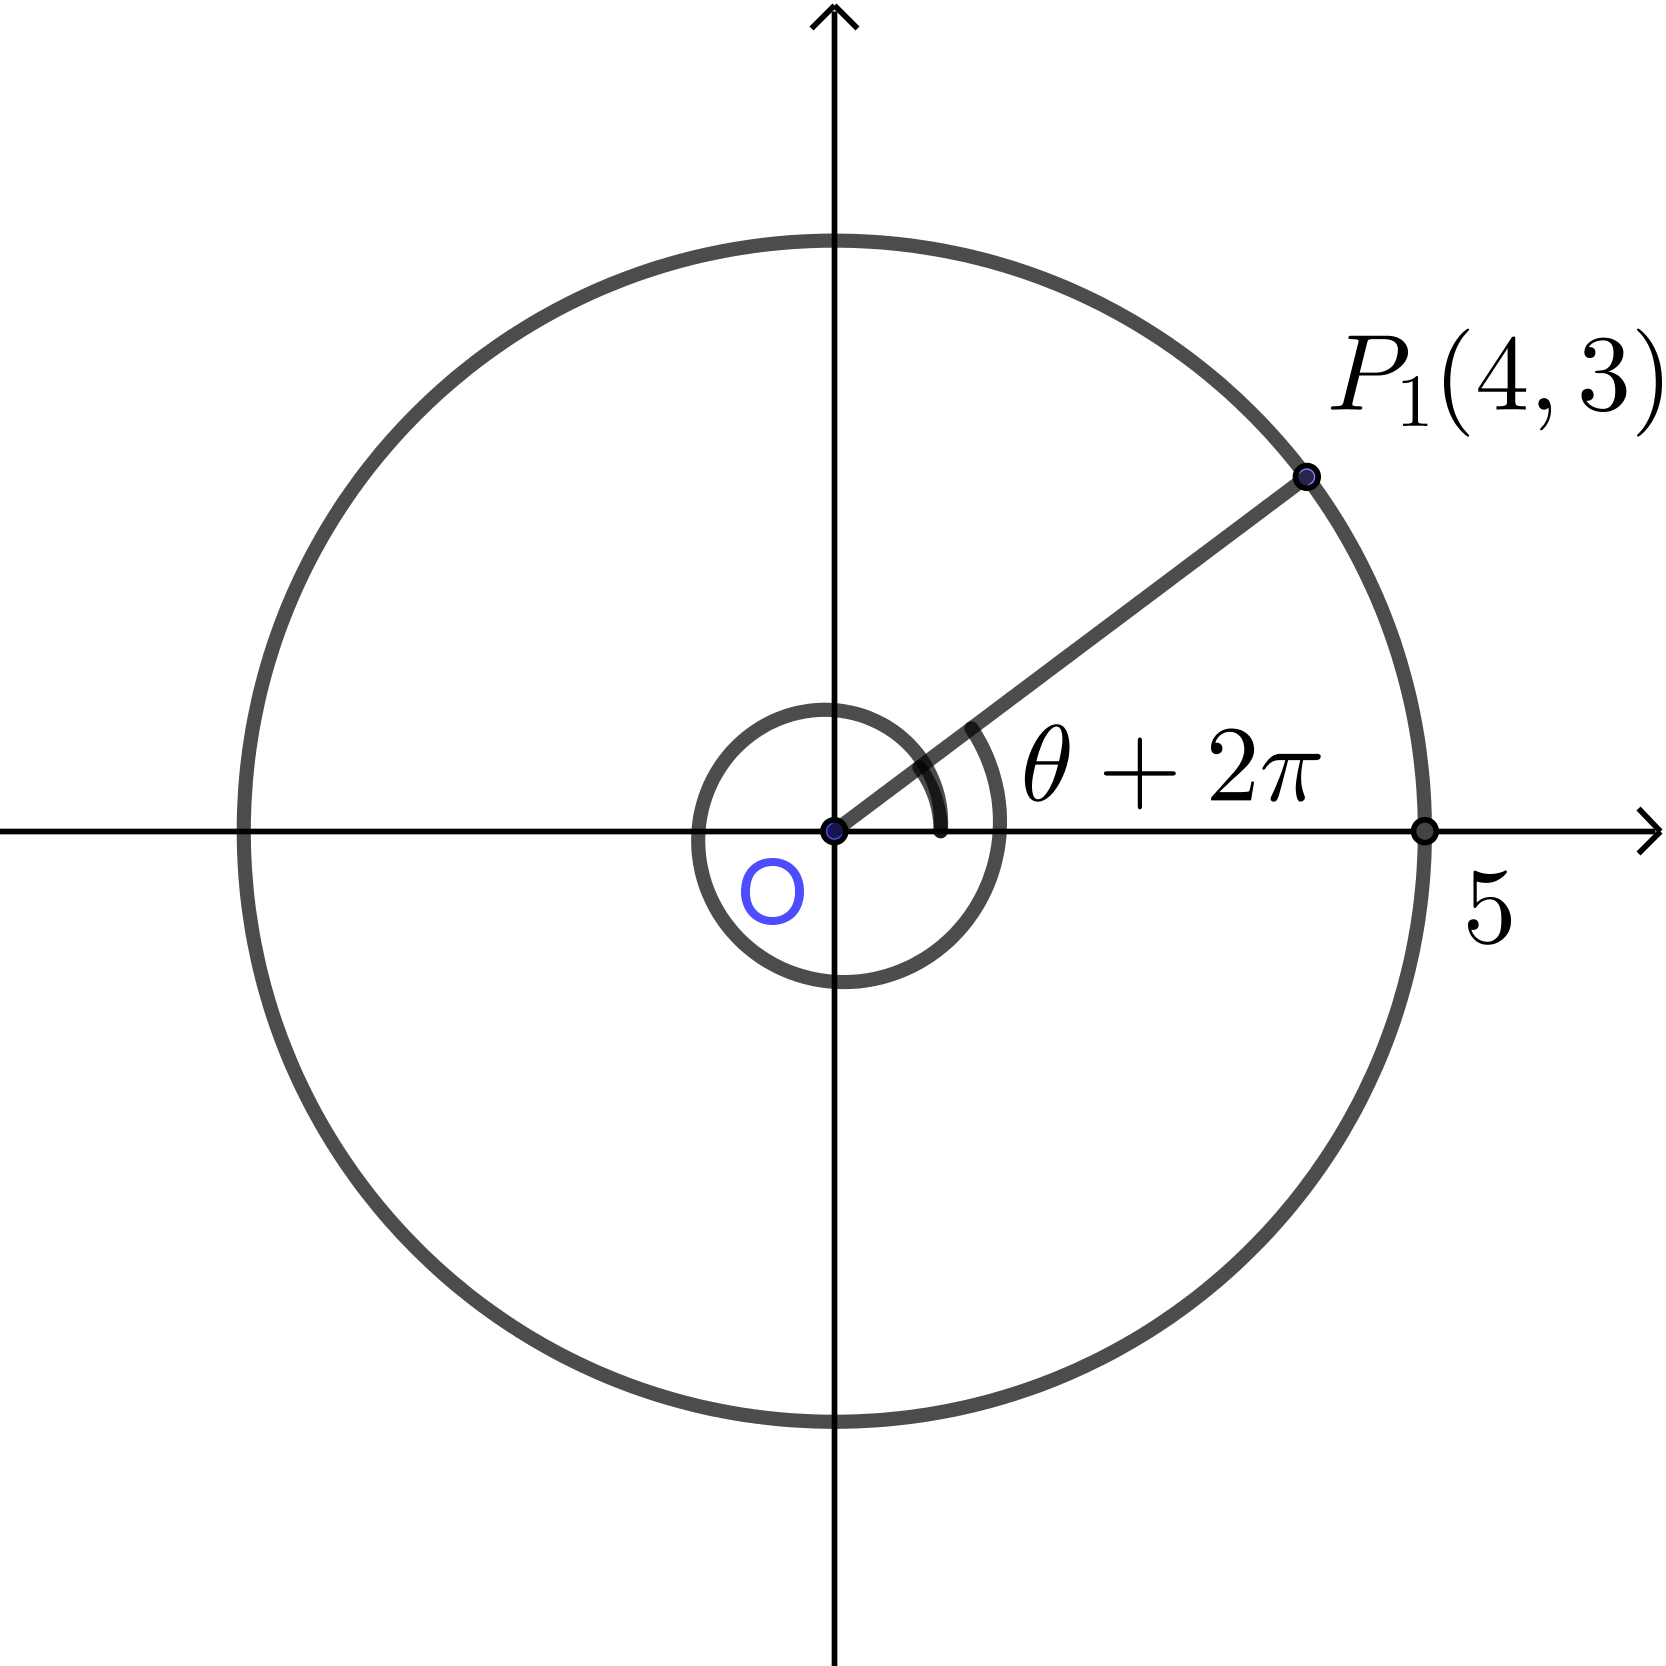
\includegraphics[width=.5\textwidth]{property_3-1}
\vspace{10pt}
\end{minipage}
\item
\(-\theta\)의 동경을 \(OP_2\)이라고 하면, \(P_2\)는 \(A\)를 시계 방향으로 \(\theta\)만큼 회전시킨 점이므로 \(P_1=(4,-3)\)이다.
\par\noindent
\begin{minipage}{.5\textwidth}
\begin{talign*}
\sin(-\theta)&=-\frac35\\
\cos(-\theta)&=\frac45\\
\tan(-\theta)&=-\frac34
\end{talign*}
\end{minipage}
\begin{minipage}{.5\textwidth}
\vspace{10pt}
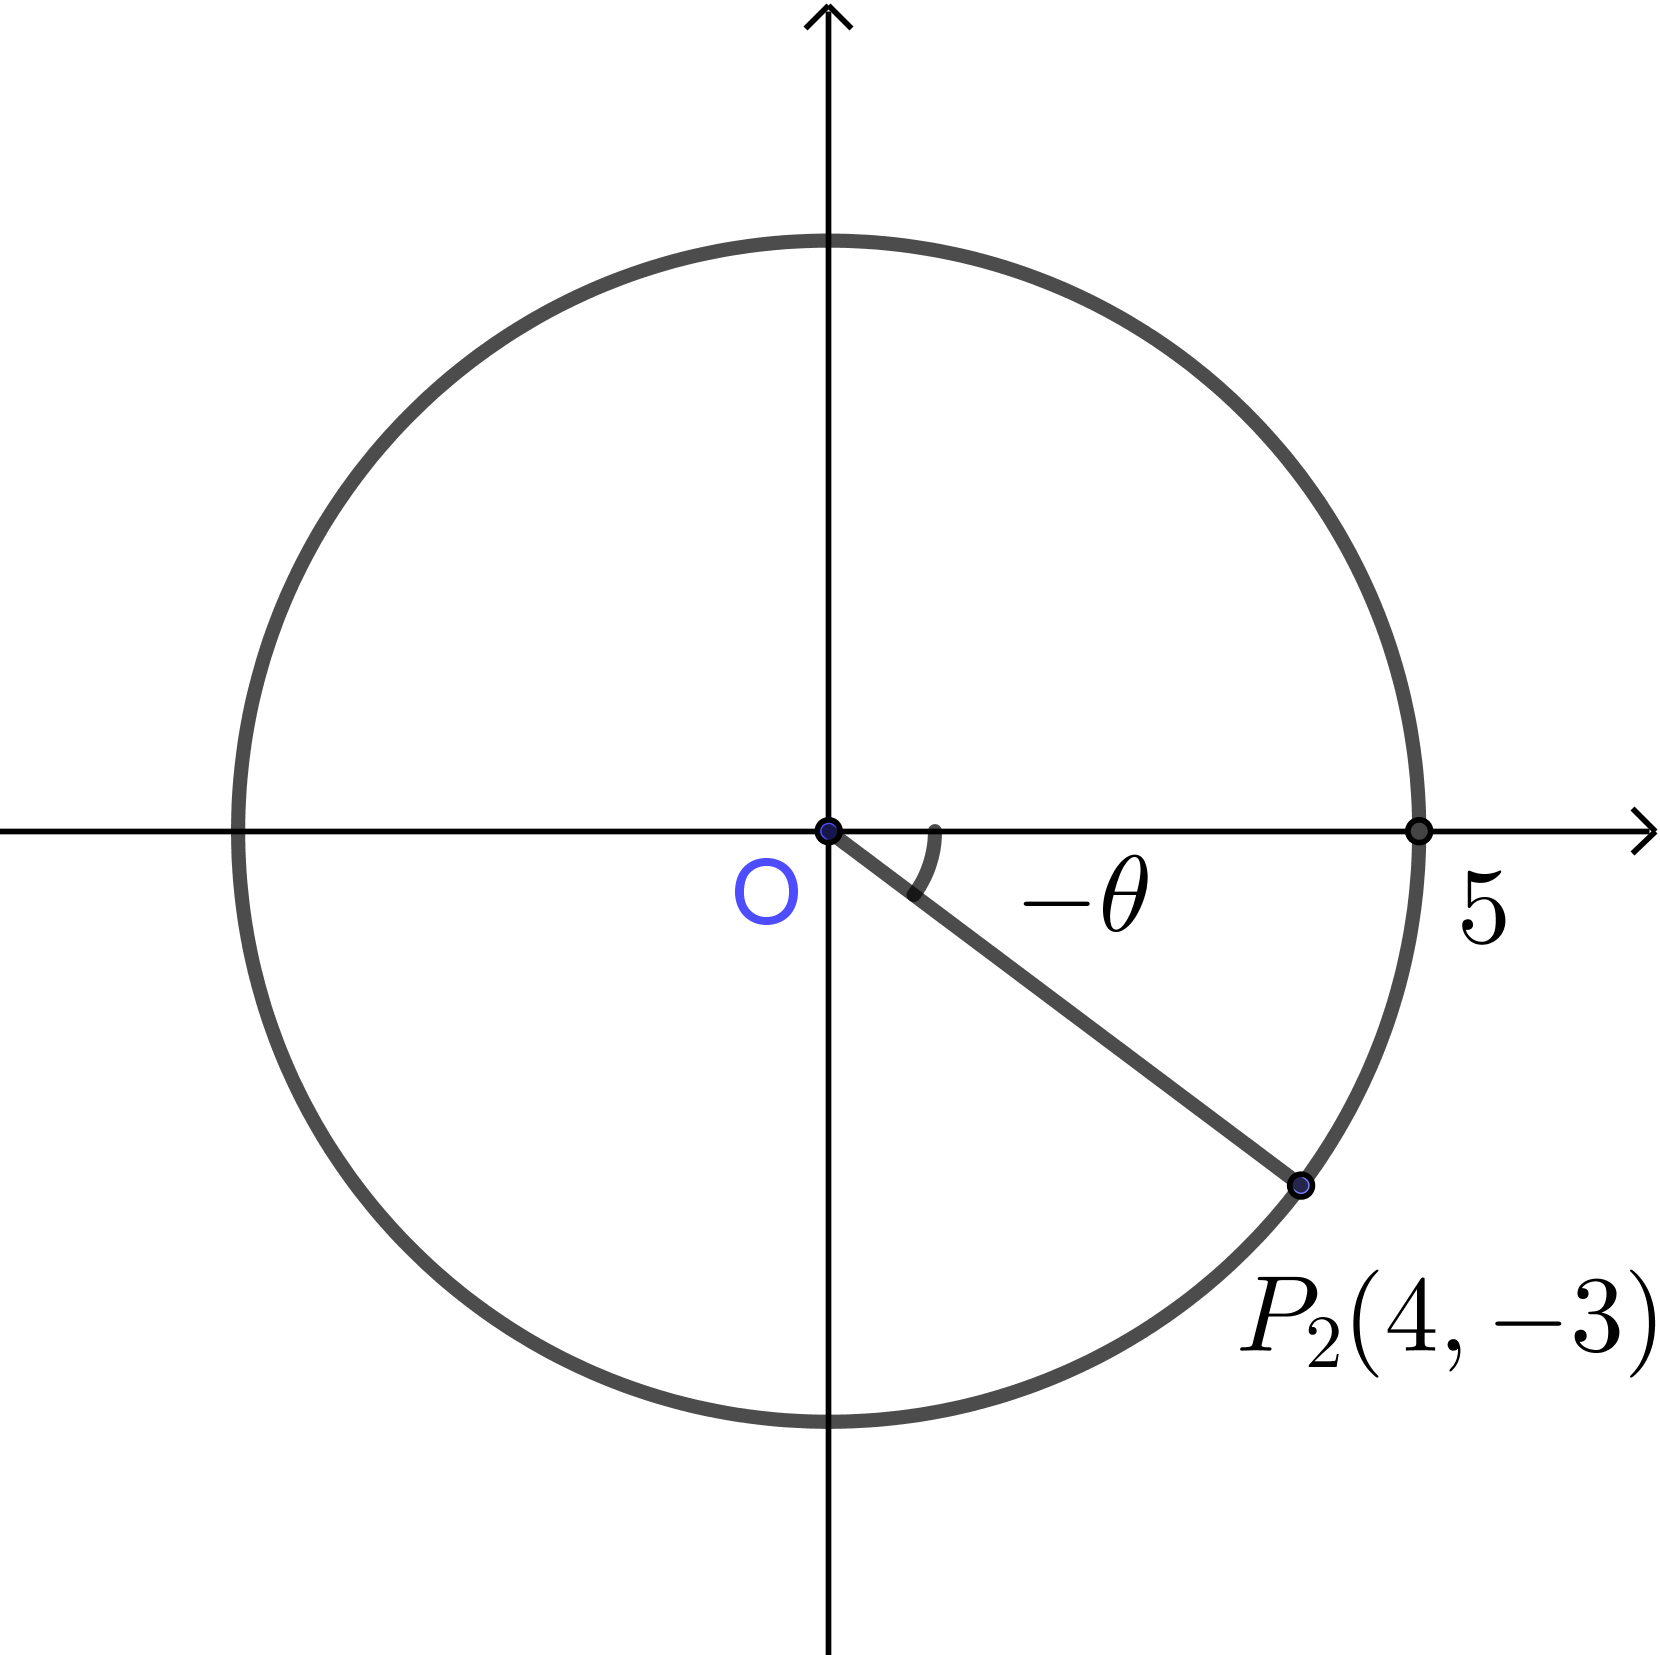
\includegraphics[width=.5\textwidth]{property_3-2}
\vspace{10pt}
\end{minipage}
\newpage
\item
\(\theta-\pi\)의 동경을 \(OP_3\)이라고 하면, \(P_3\)는 \(A\)를 시계 반대 방향으로 \(\theta\)만큼 회전시킨 후(\(=P\)), 다시 시계방향으로 \(\pi\)만큼 회전시킨 점이다.
따라서 \(P=(-4,-3)\)이다.
\par\noindent
\begin{minipage}{.5\textwidth}
\begin{talign*}
\sin(\theta-\pi)&=-\frac35\\
\cos(\theta-\pi)&=-\frac45\\
\tan(\theta-\pi)&=\frac34
\end{talign*}
\end{minipage}
\begin{minipage}{.5\textwidth}
\vspace{10pt}
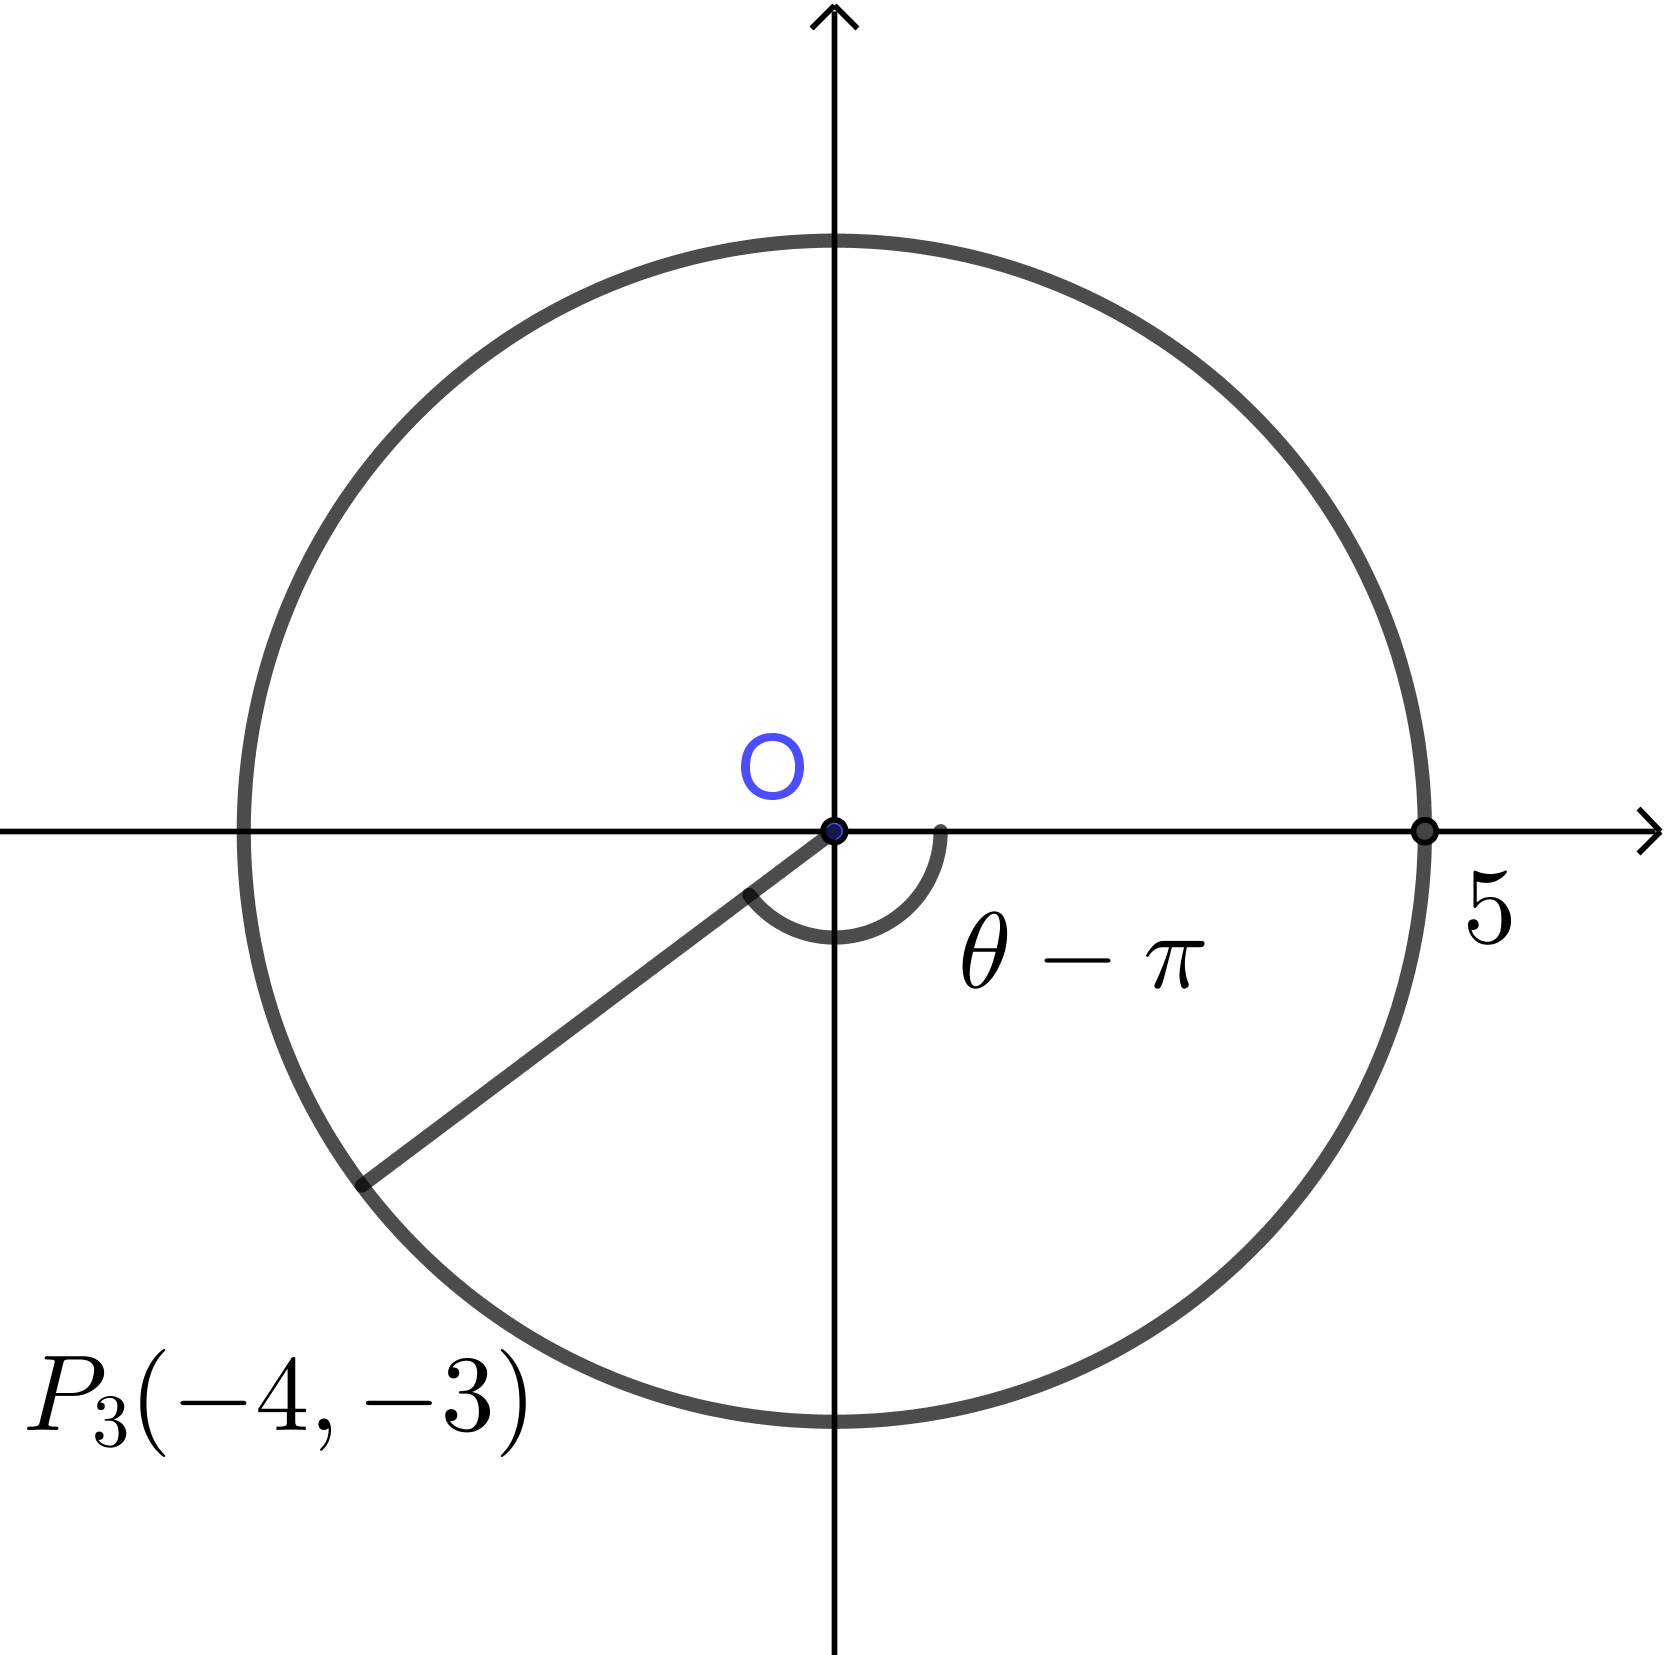
\includegraphics[width=.5\textwidth]{property_3-3}
\vspace{10pt}
\end{minipage}
\item
\(\frac\pi2-\theta\)의 동경을 \(OP_4\)이라고 하면, \(P_4\)는 \(A\)를 시계 반대 방향으로 \(\frac\pi2\)만큼 회전시킨 후, 다시 시계방향으로 \(\theta\)만큼 회전시킨 점이다.
따라서 \(P=(3,4)\)이다.
\par\noindent
\begin{minipage}{.5\textwidth}
\begin{talign*}
\sin(\frac\pi2-\theta)&=\frac45\\
\cos(\frac\pi2-\theta)&=\frac35\\
\tan(\frac\pi2-\theta)&=\frac43
\end{talign*}
\end{minipage}
\begin{minipage}{.5\textwidth}
\vspace{10pt}
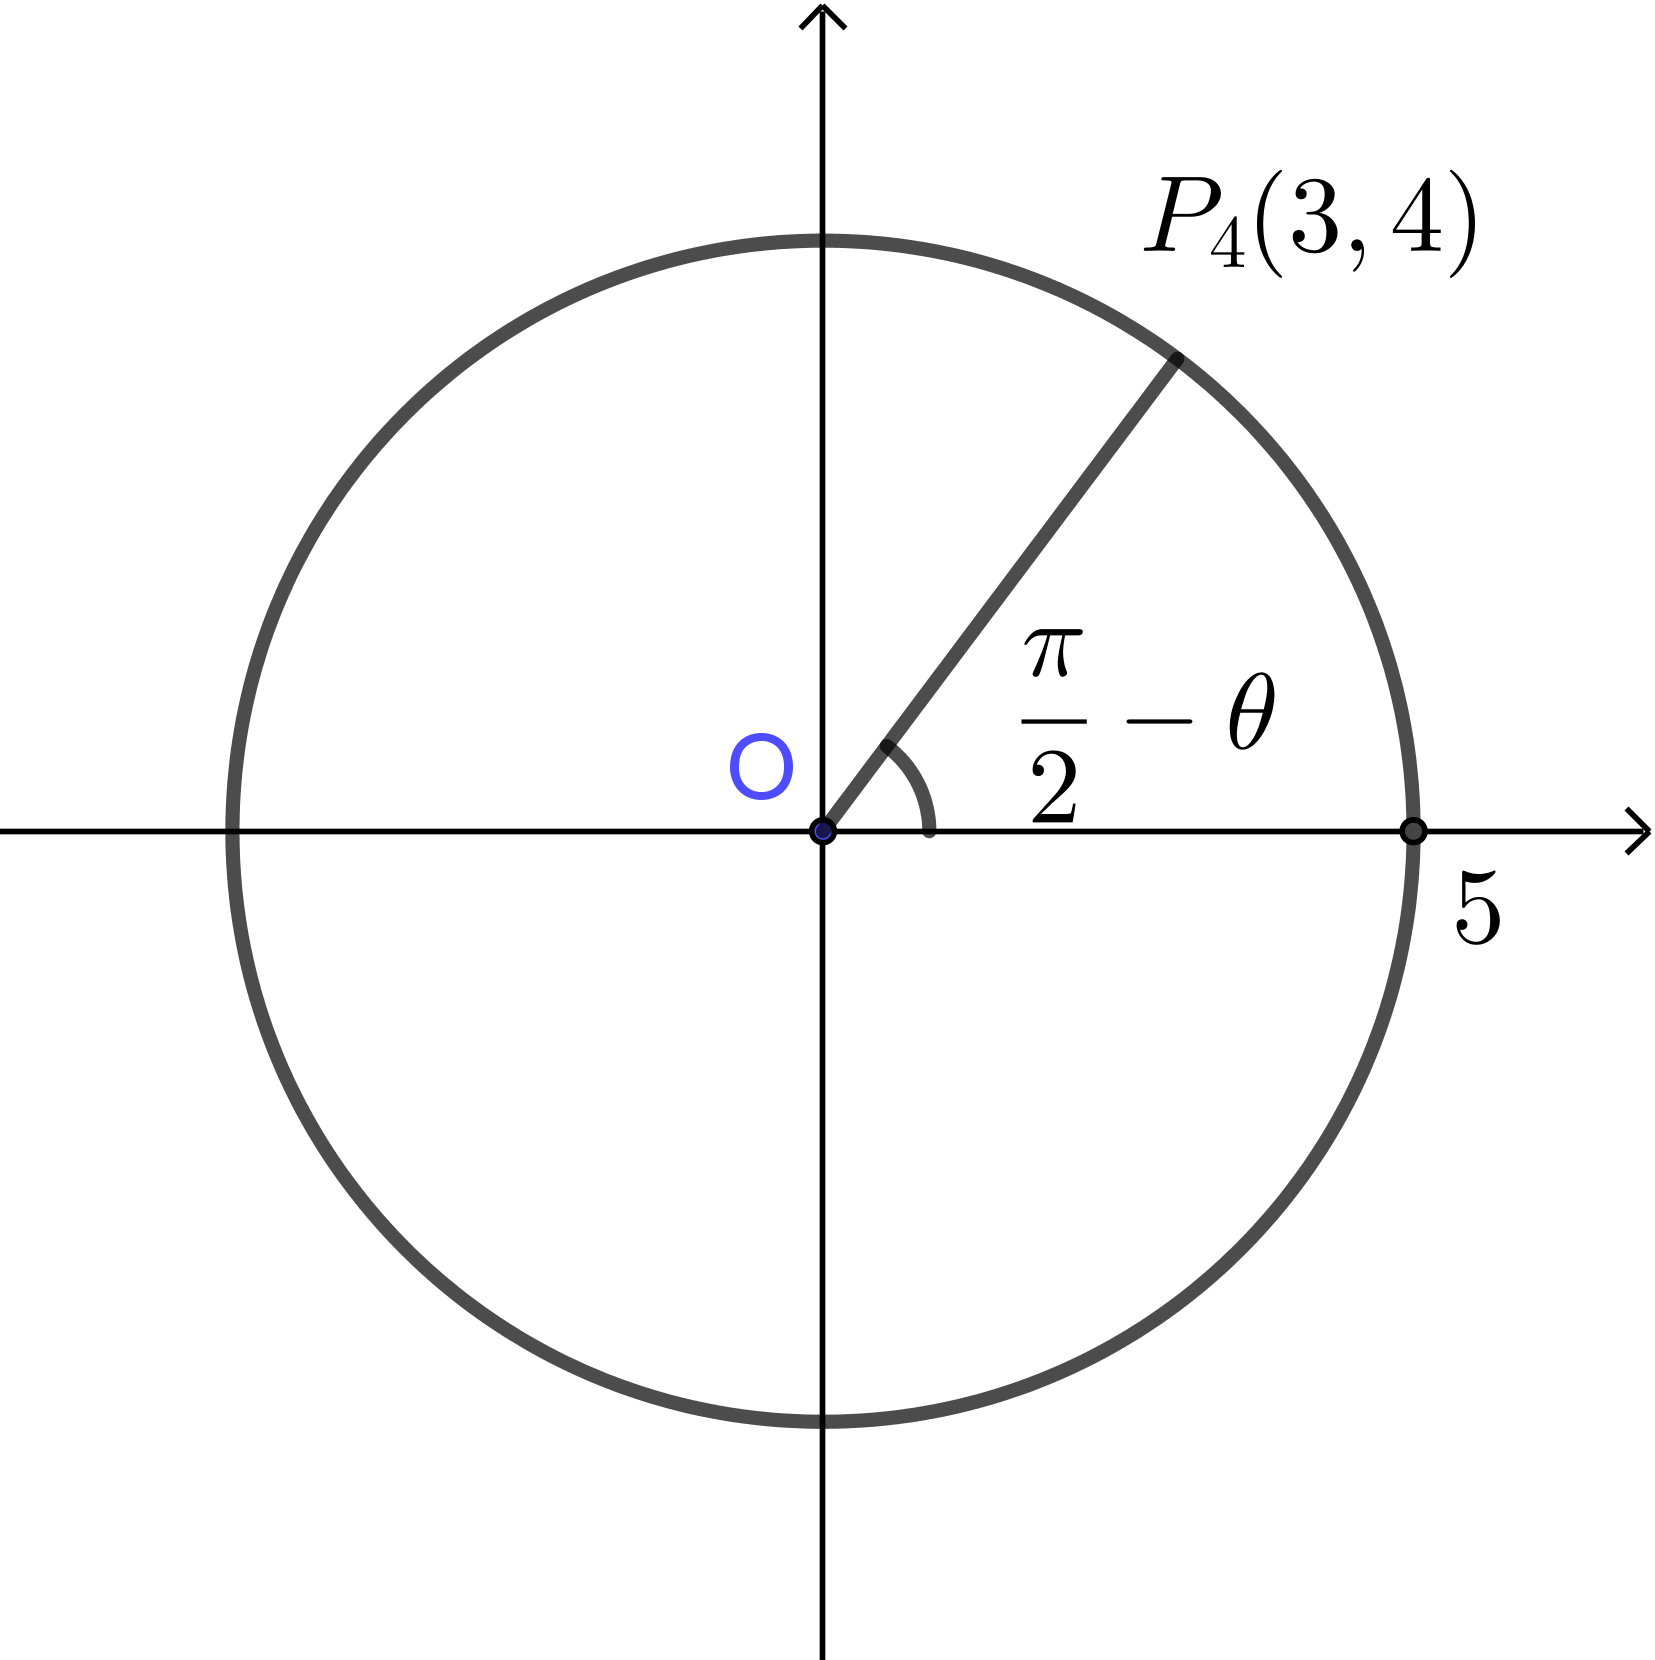
\includegraphics[width=.5\textwidth]{property_3-4}
\vspace{10pt}
\end{minipage}
\end{enumerate}
\end{mdframed}

%
\prob{각도 \(\theta\)의 동경을 \(OP\)라고 할 때, \(P=(5,12)\)이다.}\label{property4}
\par\noindent
\begin{minipage}{.5\textwidth}
\begin{talign*}
\sin\theta&=\frac{12}{13}\\
\cos\theta&=\frac5{13}\\
\tan\theta&=\frac{12}5
\end{talign*}
\end{minipage}
\begin{minipage}{.5\textwidth}
\vspace{10pt}
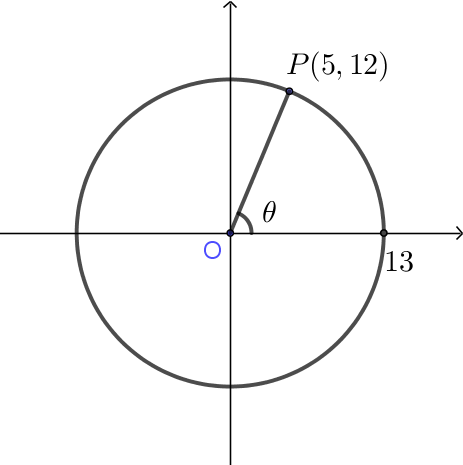
\includegraphics[width=.5\textwidth]{property_4}
\vspace{10pt}
\end{minipage}
\noindent
이때 다음 각도들에 대한 삼각비의 값을 차례로 구하여라.\\[10pt]
\begin{enumerate*}[itemjoin=\qquad\qquad]
\item
\(\theta+4\pi\)
\item
\(-\theta\)
\item
\(\theta+\pi\)
\item
\(\frac\pi2-\theta\)
\end{enumerate*}

\begin{enumerate}
\item
\begin{minipage}{.5\textwidth}
\begin{talign*}
\sin(\theta+4\pi)=&\\
\cos(\theta+4\pi)=&\\
\tan(\theta+4\pi)=&\\
\end{talign*}
\end{minipage}
\begin{minipage}{.5\textwidth}
\vspace{10pt}
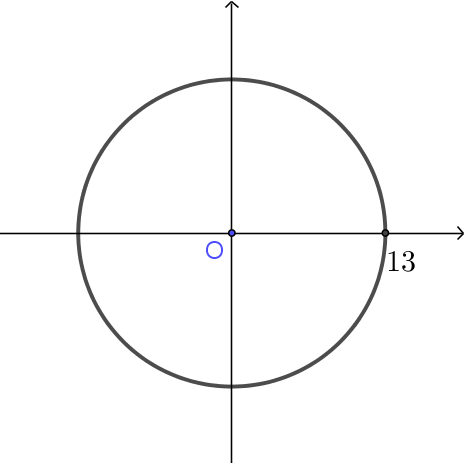
\includegraphics[width=.5\textwidth]{property_4-0}
\vspace{10pt}
\end{minipage}
\item
\begin{minipage}{.5\textwidth}
\begin{talign*}
\sin(-\theta)=&\\
\cos(-\theta)=&\\
\tan(-\theta)=&\\
\end{talign*}
\end{minipage}
\begin{minipage}{.5\textwidth}
\vspace{10pt}
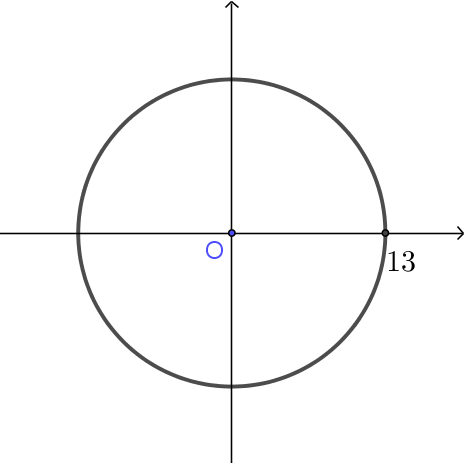
\includegraphics[width=.5\textwidth]{property_4-0}
\vspace{10pt}
\end{minipage}
\item
\begin{minipage}{.5\textwidth}
\begin{talign*}
\sin(\theta+\pi)=&\\
\cos(\theta+\pi)=&\\
\tan(\theta+\pi)=&\\
\end{talign*}
\end{minipage}
\begin{minipage}{.5\textwidth}
\vspace{10pt}
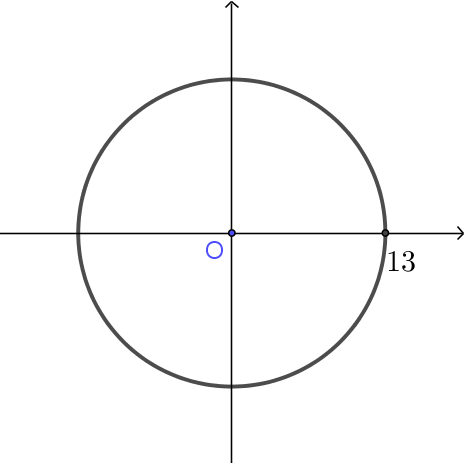
\includegraphics[width=.5\textwidth]{property_4-0}
\vspace{10pt}
\end{minipage}
\item
\begin{minipage}{.5\textwidth}
\begin{talign*}
\sin(\frac\pi2-\theta)=&\\
\cos(\frac\pi2-\theta)=&\\
\tan(\frac\pi2-\theta)=&\\
\end{talign*}
\end{minipage}
\begin{minipage}{.5\textwidth}
\vspace{10pt}
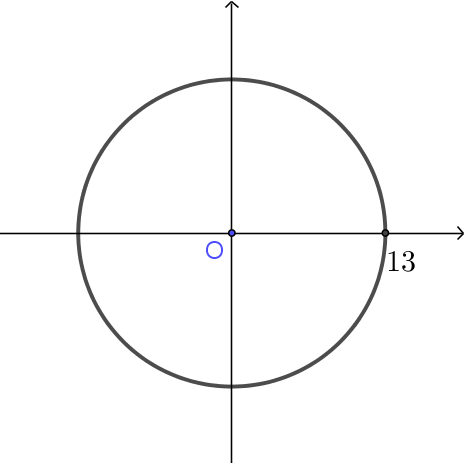
\includegraphics[width=.5\textwidth]{property_4-0}
\vspace{10pt}
\end{minipage}
\end{enumerate}

%%%
\section{삼각함수의 그래프}
\vspace{-20pt}
%
\prob{다음 표를 완성하여라.}\label{graph1}\\[-5pt]
\begin{tabu}{|@{}X[2c$]@{}|@{}X[c$]@{}|@{}X[c$]@{}|@{}X[c$]@{}|@{}X[c$]@{}|@{}X[c$]@{}|@{}X[c$]@{}|@{}X[c$]@{}|@{}X[c$]@{}|@{}X[c$]@{}|@{}X[c$]@{}|@{}X[c$]@{}|@{}X[c$]@{}|@{}X[c$]@{}|}
\hline
\theta
&0
&\frac\pi6
&\frac\pi3
&\frac\pi2
&\frac23\pi
&\frac56\pi
&\pi
&\frac76\pi
&\frac43\pi
&\frac32\pi
&\frac53\pi
&\frac{11}6\pi
&2\pi
\\\hline
\sin\theta
&&\frac12&&&&&&&&&&&
\\\hline
\cos\theta
&&\frac{\sqrt3}2&&&&&&&&&&&
\\\hline
\tan\theta
&&\frac{\sqrt3}3&&&&&&&&&&&
\\\hline
\end{tabu}
\par\bigskip\noindent
위의 표를 참고하여 \(y=\sin x\), \(y=\cos x\), \(y=\tan x\)의 그래프를 그려라.%}\label{graph2}
\begin{figure*}[h!]
\centering
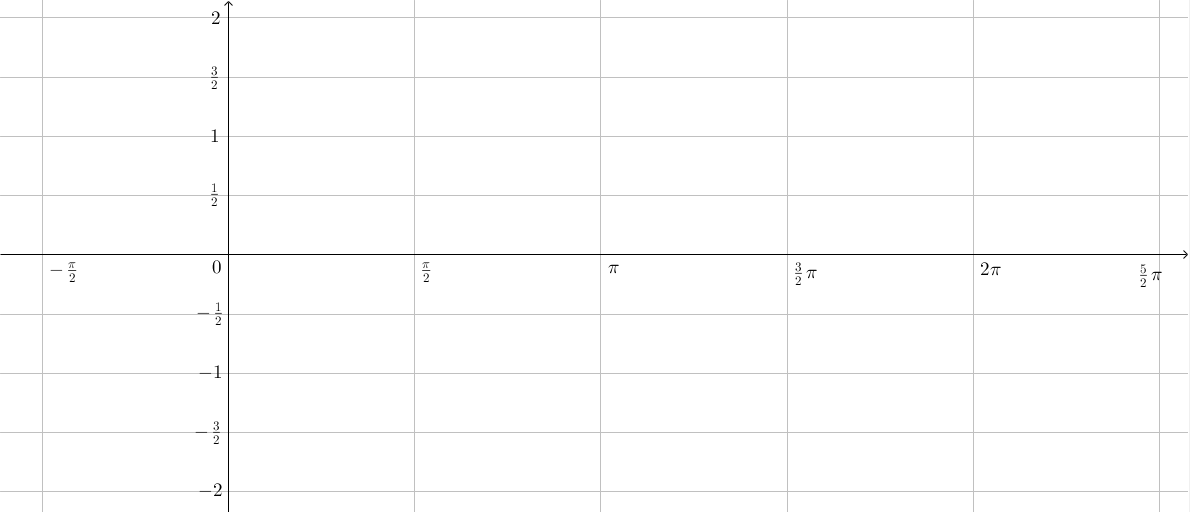
\includegraphics[width=\textwidth]{graph_grid}
\caption*{\(y=\sin x\)}
\end{figure*}

\begin{figure*}[h!]
\centering
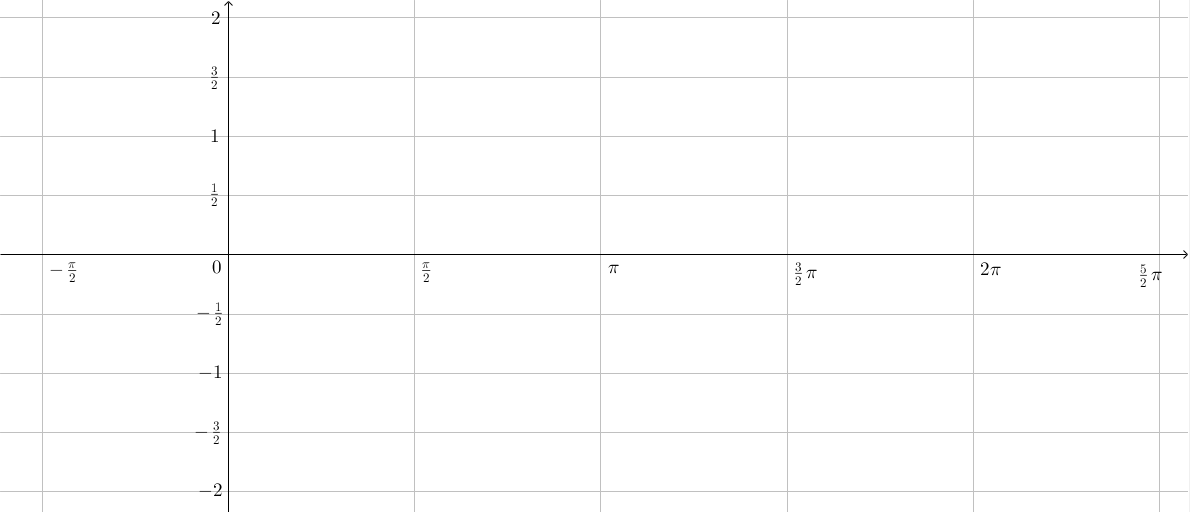
\includegraphics[width=\textwidth]{graph_grid}
\caption*{\(y=\cos x\)}
\end{figure*}

\begin{figure*}[h!]
\centering
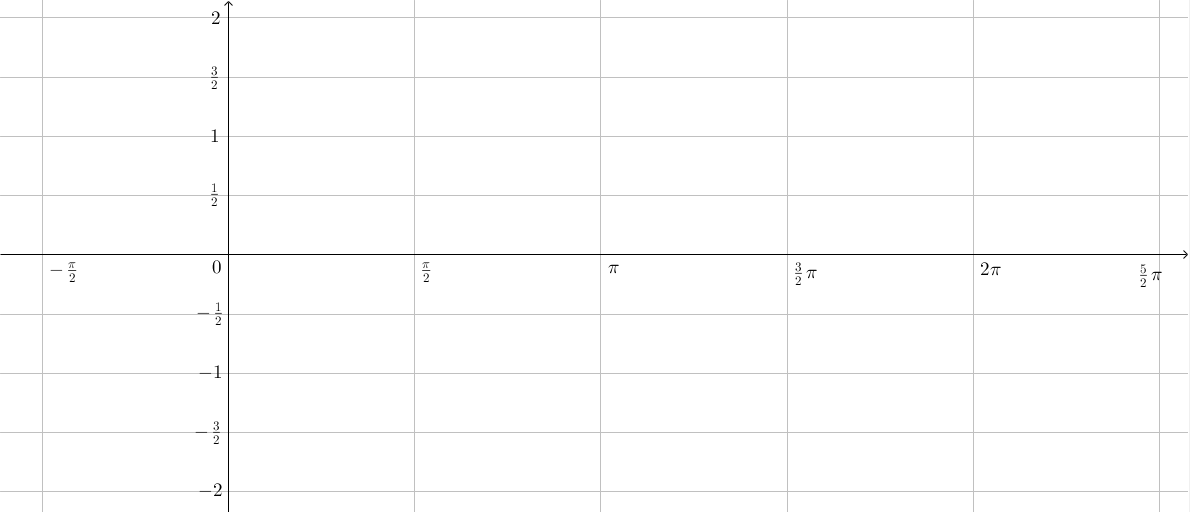
\includegraphics[width=\textwidth]{graph_grid}
\caption*{\(y=\tan x\)}
\end{figure*}

\newpage
%
\theo{삼각함수의 그래프}\label{graph2}\\[-5pt]
\begin{tabu}{>{\small}X[c]>{\small}X[c]|>{\small}X[1.5,c]}
\tabucline [1pt]{-}
\(y=\sin x\)			&\(y=\cos x\)						&\(y=\tan x\)\\\tabucline [1pt]{-}
\multicolumn{2}{c|}{\small정의역은 실수 전체의 집합이다.}	&정의역은 \(\{x\ba x\neq n\pi+\frac\pi2\}\)이다.\\\tabucline[.2pt]{-}
\multicolumn{2}{c|}{\small치역은 \(\{y\ba-1\le y\le 1\}\)이다.}	&치역은 실수 전체의 집합이다.\\\tabucline[.2pt]{-}
\multicolumn{2}{c|}{\small최댓값이 1이고 최솟값이 \(-1\)이다.}	&최댓값과 최솟값이 없다.\\\tabucline [1pt]{-}
\(\sin(x+2\pi)=\sin x\)	&\(\cos(x+2\pi)=\cos x\)				&\(\tan(x+\pi)=\tan x\)\\\tabucline[.2pt]{-}
\multicolumn{2}{c|}{\small주기가 \(2\pi\)인 함수이다.}			&주기가 \(\pi\)인 함수이다.\\\tabucline [1pt]{-}
\(\sin(-x)=-\sin x\) 		&\(\cos(-x)=\cos x\)					&\(\tan(-x)=-\tan x\)\\\tabucline[.2pt]{-}
원점 대칭이다.		&\(y\)축 대칭이다.					&원점 대칭이다.\\\tabucline[.2pt]{-}
기함수이다.			&우함수이다.						&기함수이다.\\\tabucline [1pt]{-}
\multicolumn{2}{c|}{점근선이 없다.}						&점근선 \(x=n\pi+\frac\pi2\)을 가진다.\\\tabucline [1pt]{-}
\end{tabu}

\newpage
%
\exam{다음 삼각함수들의 그래프를 그려라.}
\begin{enumerate}\label{graph3}
\item
\(y=\sin(x-\frac\pi4)\)
\par\noindent
\(y=\sin x\)의 그래프를 \(x\)축의 방향으로 \(\frac\pi4\)만큼 평행이동시키면 된다.
따라서 다음과 같은 그래프가 나온다.
\begin{figure*}[h!]
\centering
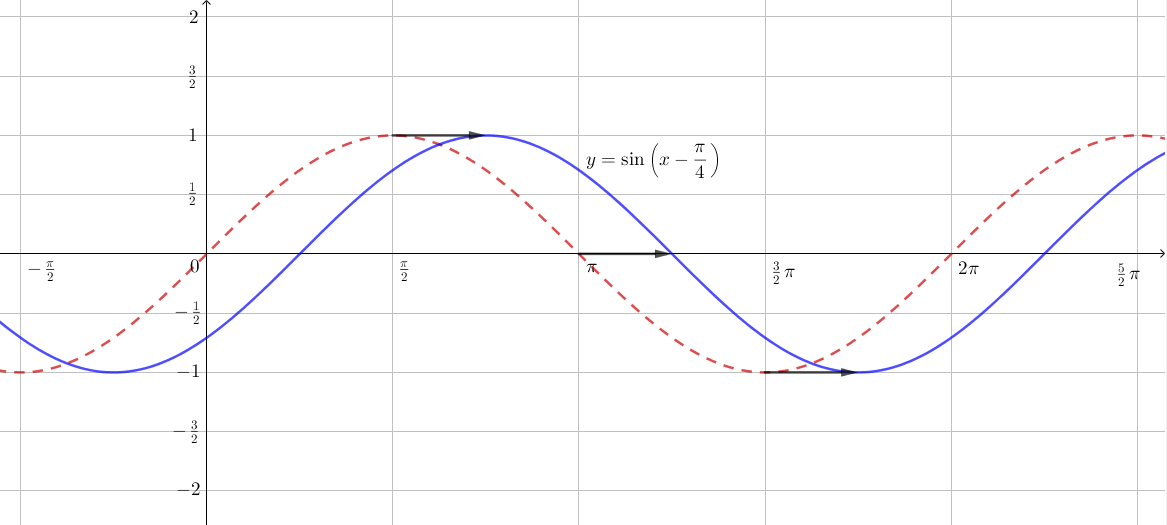
\includegraphics[width=\textwidth]{graph_3-1}
\end{figure*}
\item
\(y=\sin x-1\)
\par\noindent
\(y=\sin x\)의 그래프를 \(y\)축의 방향으로 \(-1\)만큼 평행이동시키면 된다.
따라서 다음과 같은 그래프가 나온다.
\begin{figure*}[h!]
\centering
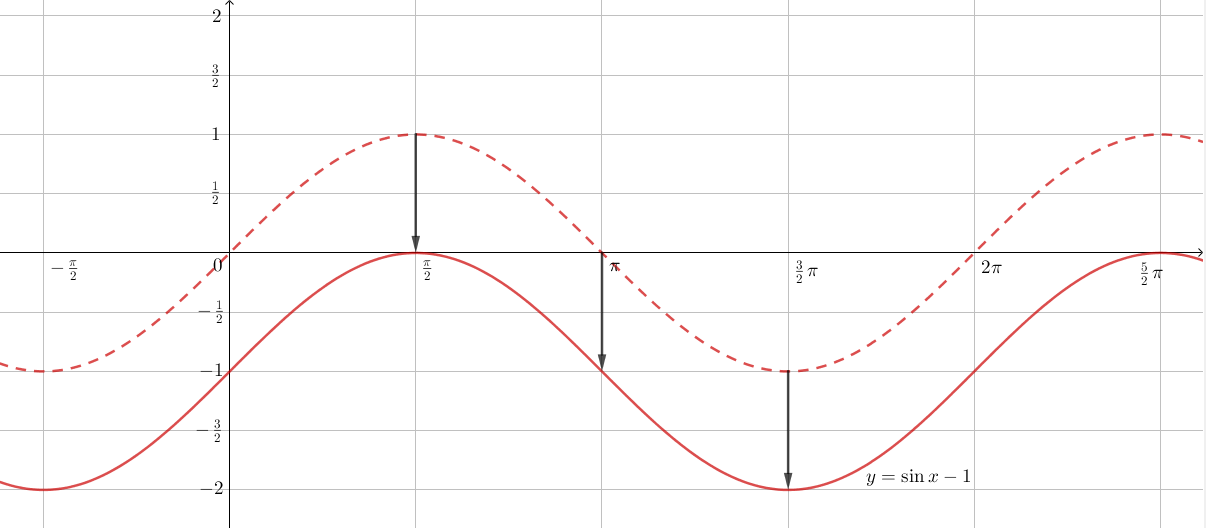
\includegraphics[width=\textwidth]{graph_3-2}
\end{figure*}
\end{enumerate}

\newpage
%
\prob{다음 삼각함수들의 그래프를 그려라.}
\begin{enumerate}\label{graph4}
\item
\(y=2\sin x\)
\par\noindent
\begin{tabu}{|@{}X[2c$]@{}|@{}X[c$]@{}|@{}X[c$]@{}|@{}X[c$]@{}|@{}X[c$]@{}|@{}X[c$]@{}|@{}X[c$]@{}|@{}X[c$]@{}|@{}X[c$]@{}|@{}X[c$]@{}|@{}X[c$]@{}|@{}X[c$]@{}|@{}X[c$]@{}|@{}X[c$]@{}|}
\hline
x&0&\frac\pi6&\frac\pi3&\frac\pi2&\frac23\pi&\frac56\pi&\pi&\frac76\pi&\frac43\pi&\frac32\pi&\frac53\pi&\frac{11}6\pi&2\pi
\\\hline
2\sin x
&&&&&&&&&&&&&
\\\hline
\end{tabu}
\begin{figure*}[h!]
\centering
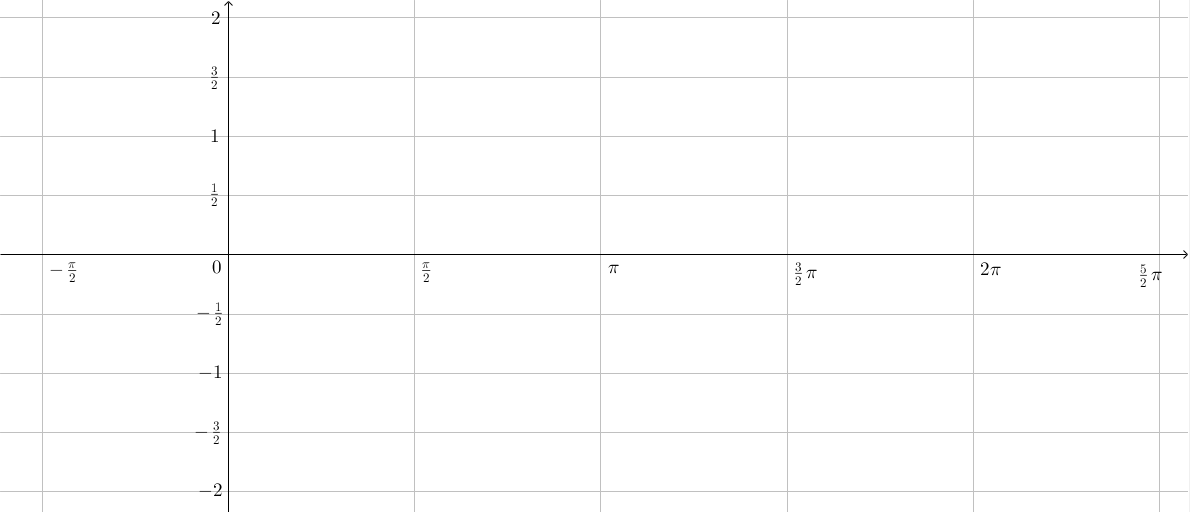
\includegraphics[width=\textwidth]{graph_grid}
\end{figure*}
\item
\(y=\sin 2x\)
\par\noindent
\begin{tabu}{|@{}X[2c$]@{}|@{}X[c$]@{}|@{}X[c$]@{}|@{}X[c$]@{}|@{}X[c$]@{}|@{}X[c$]@{}|@{}X[c$]@{}|@{}X[c$]@{}|@{}X[c$]@{}|@{}X[c$]@{}|@{}X[c$]@{}|@{}X[c$]@{}|@{}X[c$]@{}|@{}X[c$]@{}|}
\hline
x&0&\frac\pi6&\frac\pi3&\frac\pi2&\frac23\pi&\frac56\pi&\pi&\frac76\pi&\frac43\pi&\frac32\pi&\frac53\pi&\frac{11}6\pi&2\pi
\\\hline
\sin 2x
&&&&&&&&&&&&&
\\\hline
\end{tabu}
\begin{figure*}[h!]
\centering
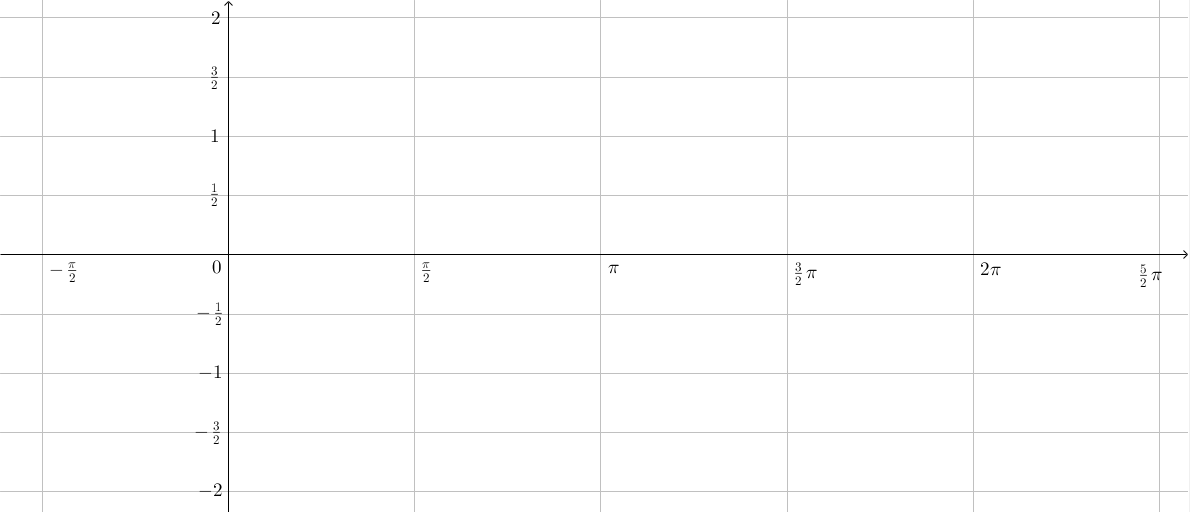
\includegraphics[width=\textwidth]{graph_grid}
\end{figure*}
\end{enumerate}

\newpage
예시 \ref{property3})과 문제 \ref{property4})에서 우리는 다음과 같은 성질들을 유추할 수 있었다.
\begin{mdframed}
%
\theo{}
\begin{enumerate}\label{graph5}
\item
\(\sin(x+2\pi)=\sin x\), \(\cos(x+2\pi)=\cos x\), \(\tan(x+2\pi)=\tan x\)
\item
\(\sin(-x)=-\sin x\), \(\cos(-x)=\cos x\), \(\tan(-x)=-\tan x\)
\item
\(\sin(x+\pi)=-\sin x\), \(\cos(x+\pi)=-\cos x\), \(\tan(x+\pi)=\tan x\)
\item
\(\sin(\frac\pi2-x)=\cos x\), \(\cos(\frac\pi2-x)=\sin x\)
\end{enumerate}
\end{mdframed}
이 성질들은 삼각함수의 그래프를 통해서 보면 더 명확하게 보인다.

\bigskip
(1)은 삼각함수가 일정한 주기를 가진다는 사실로부터, (2)는 삼각함수가 원점 혹은 \(y\)축을 기준으로 대칭성이 있다는 사실로부터 당연하다.

\bigskip
한편 \(y=\sin x\)의 그래프를 \(x\)축의 방향으로 \(-\pi\)만큼 이동시켜 \(y=\sin(x+\pi)\)의 그래프를 그리면, 정확히 \(y=-\sin x\)의 그래프와 일치한다.
코사인과 탄젠트의 경우도 마찬가지이다.
따라서 (3)이 성립한다.
\begin{center}
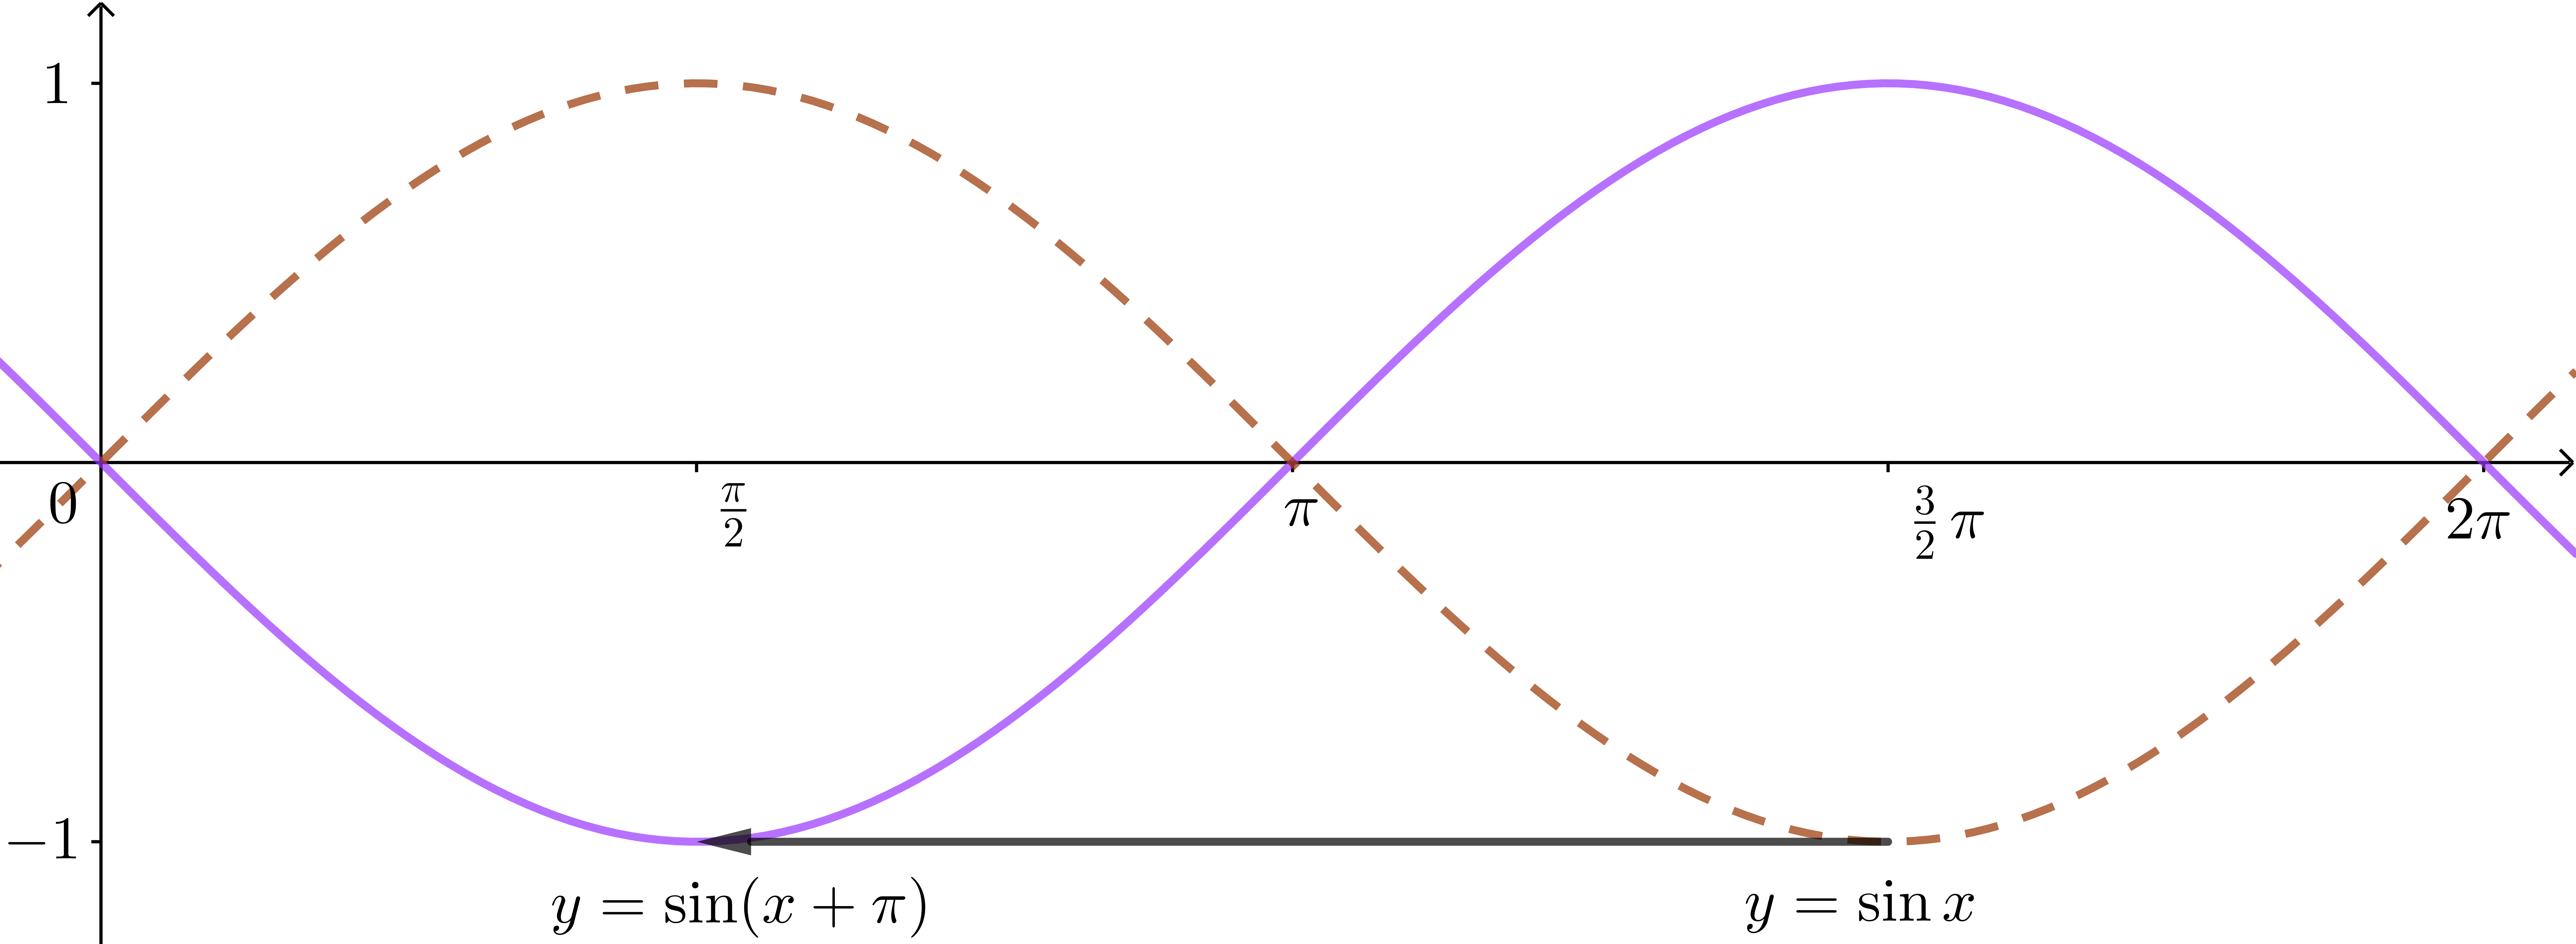
\includegraphics[width=.7\textwidth]{graph_5-1}
\end{center}

\bigskip
또한 \(y=\sin x\)의 그래프를 \(y\)축 대칭이동시켜 \(y=\sin(-x)\)그래프를 얻고, 이것을 다시 \(x\)축의 방향으로 \(\frac\pi2\)만큼 이동시켜 \(y=\sin(\frac\pi2-x)\)의 그래프를 얻으면, 정확히 \(y=\cos x\)의 그래프와 일치한다.
코사인의 경우도 마찬가지이다.
따라서 (4)가 성립한다.
\begin{center}
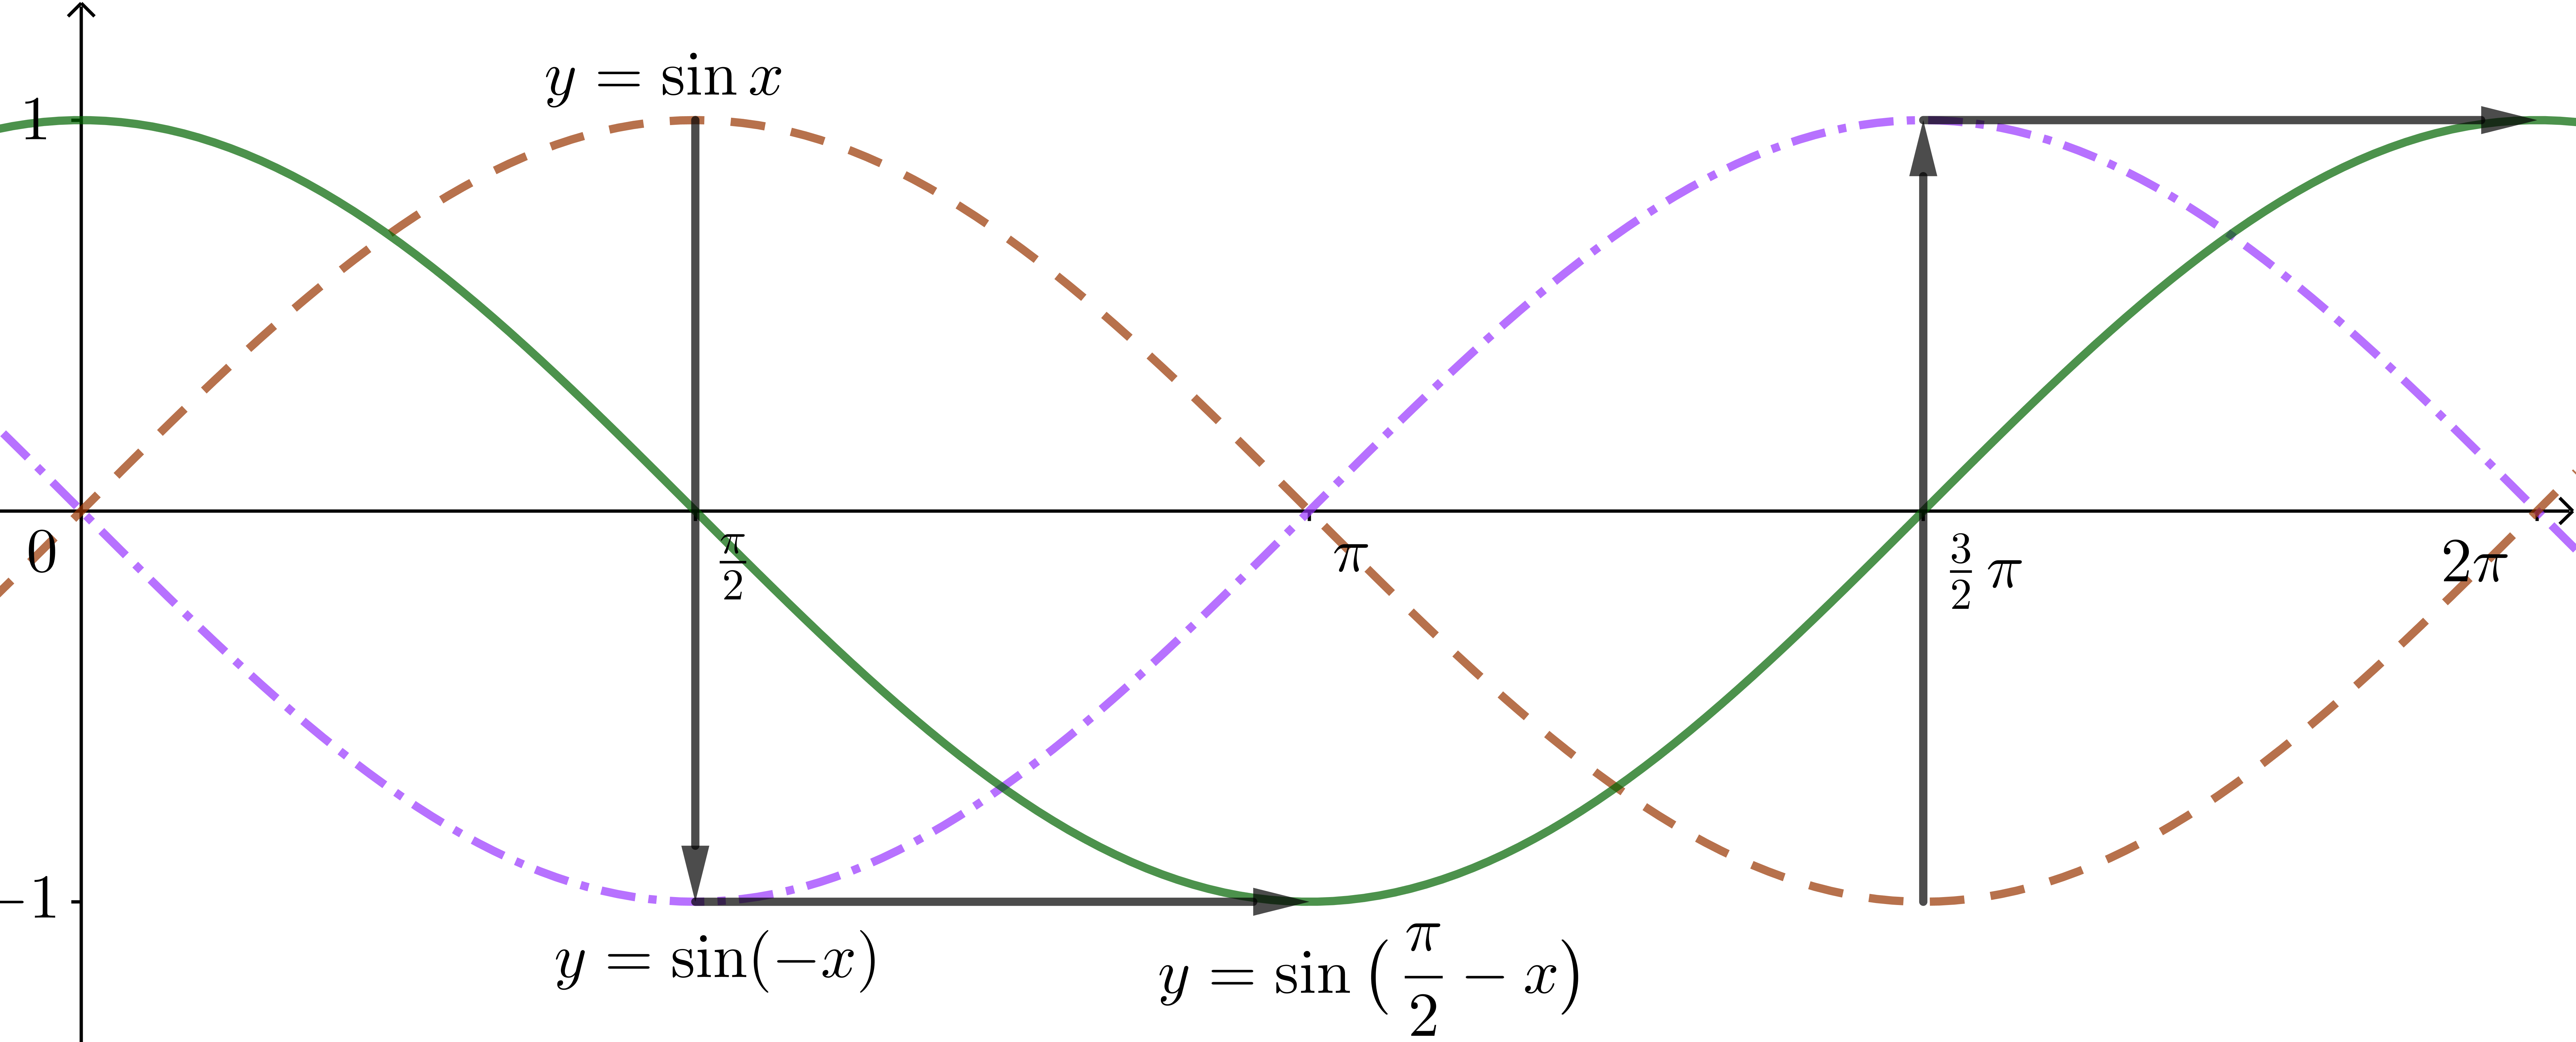
\includegraphics[width=.7\textwidth]{graph_5-2}
\end{center}

\newpage
%
\prob{삼각함수의 그래프를 이용하여 다음 등식이 성립함을 보여라.}\label{graph6}
(1)\;\;\(\sin(x+\frac\pi2)=\cos x\)
\begin{figure*}[h!]
\centering
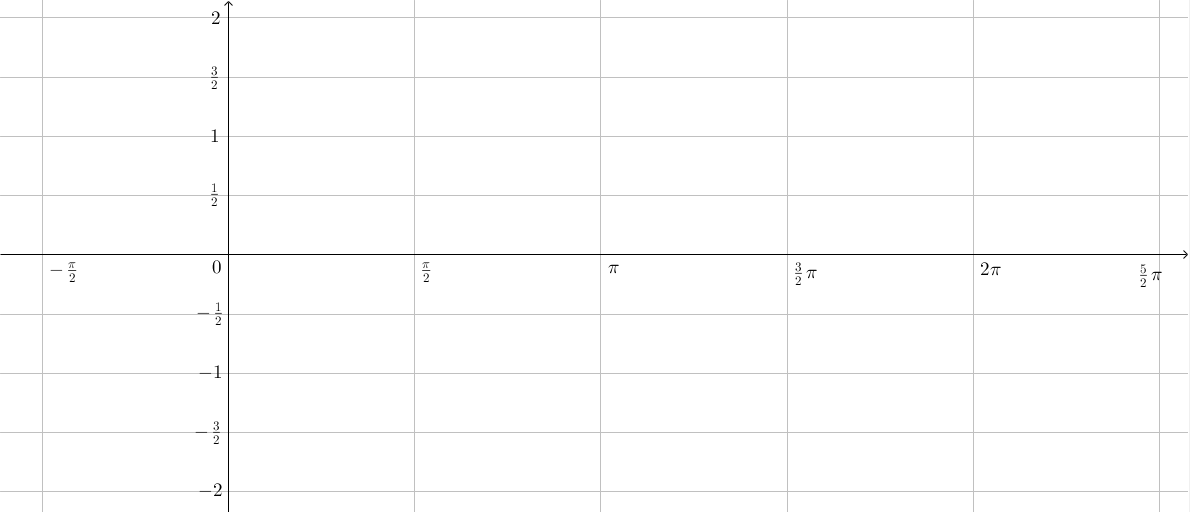
\includegraphics[width=\textwidth]{graph_grid}
%\caption*{(1)\;\;\(\sin(x+\frac\pi2)=\cos x\)}
\end{figure*}
\par\noindent
(2)\;\;\(\sin(\pi-x)=\sin x\)
\begin{figure*}[h!]
\centering
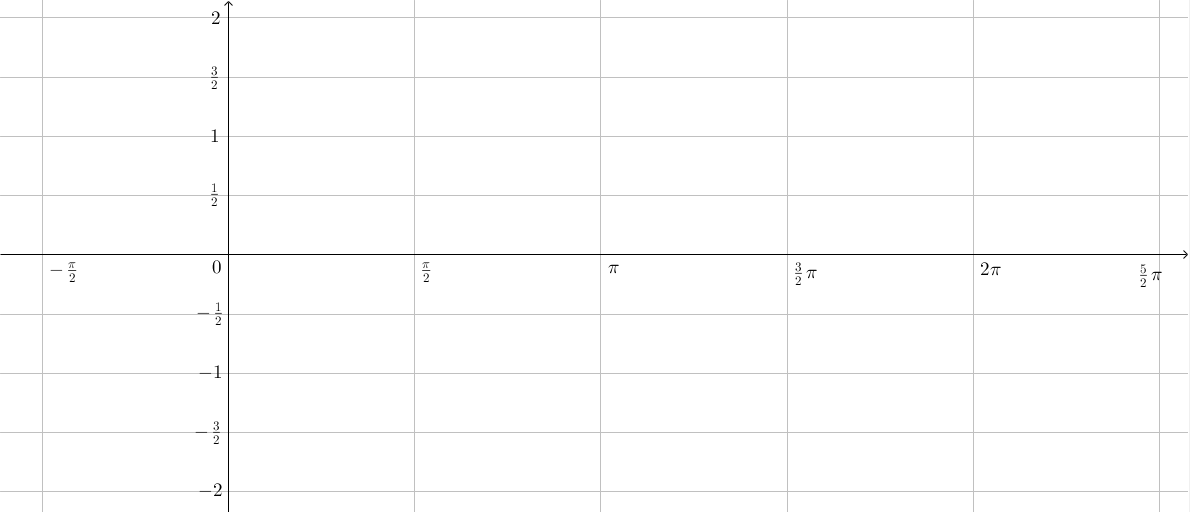
\includegraphics[width=\textwidth]{graph_grid}
%\caption*{(2)\;\;\(\cos(\pi-x)=\cos x\)}
\end{figure*}

%%%
\section{삼각방정식}

%
\exam{\(0\le x<2\pi\)일 때, 다음 방정식의 근을 구하여라.}\label{equa1}
\begin{enumerate*}[itemjoin=\tabto{.5\textwidth}]
\item
\(\cos x=\frac{\sqrt3}2\)
\item
\(\tan x=\sqrt3\)
\end{enumerate*}

\begin{mdframed}[frametitle=삼각함수의 정의를 사용하는 방법]
\begin{enumerate}
\item
\par\noindent
\begin{minipage}[t]{.6\textwidth}
원 \(x^2+y^2=1\)과 직선 \(x=\frac{\sqrt3}2\)의 교점이 \((\frac{\sqrt3}2,\frac12)\), \((\frac{\sqrt3}2,-\frac12)\)의 두 개이므로
\[x=\frac\pi6,\quad\frac{11}6\pi\]
\end{minipage}
\begin{minipage}{.4\textwidth}\centering
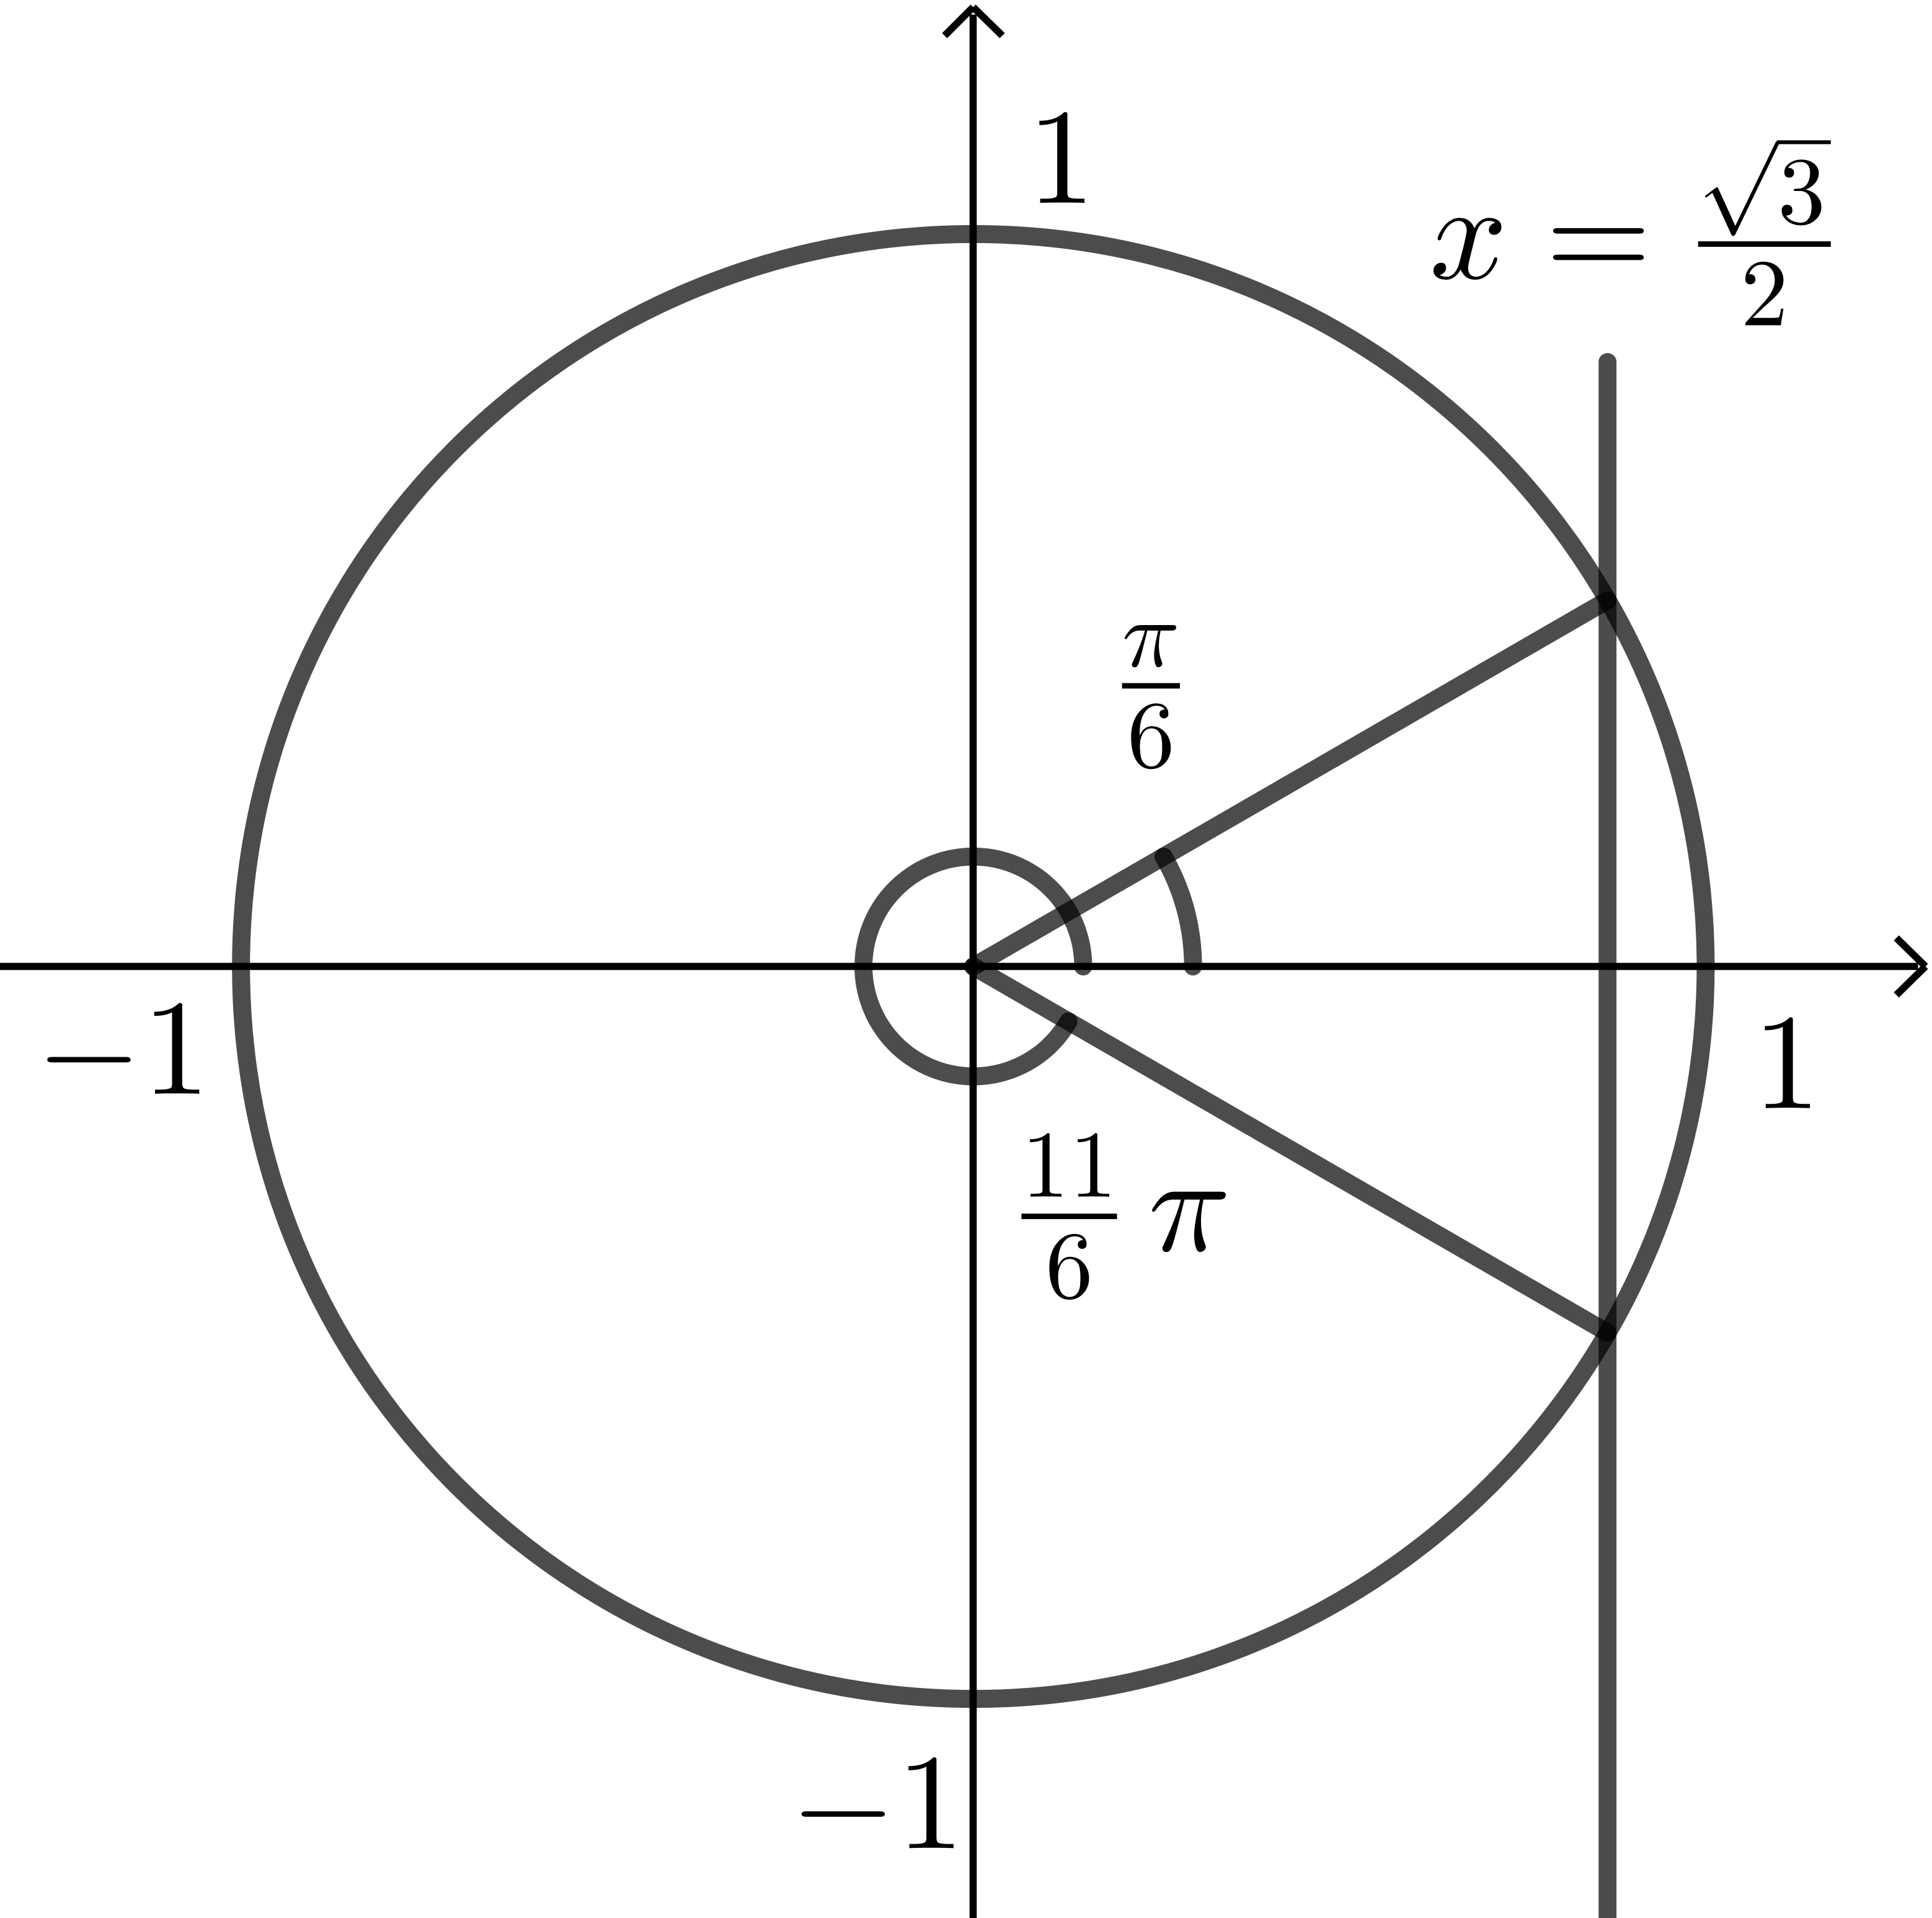
\includegraphics[width=.6\textwidth]{equa_1-1}
\end{minipage}
\item
\par\noindent
\begin{minipage}[t]{.6\textwidth}
원 \(x^2+y^2=1\)과 직선 \(y=\sqrt3x\)의 교점이 \((\frac12,\frac{\sqrt3}2)\), \((-\frac12,-\frac{\sqrt3}2)\)의 두 개이므로
\[x=\frac\pi3,\quad\frac43\pi\]
\end{minipage}
\begin{minipage}{.4\textwidth}\centering
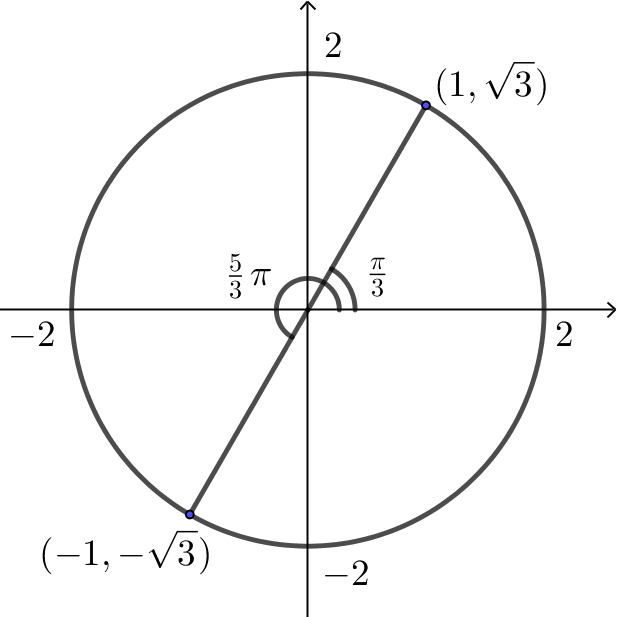
\includegraphics[width=.6\textwidth]{equa_1-2}
\end{minipage}
\end{enumerate}
\end{mdframed}

\begin{mdframed}[frametitle=그래프를 사용하는 방법,nobreak=false]
\begin{enumerate}
\item
\(y=\cos x\)의 그래프와 \(y=\frac{\sqrt3}2\)의 교점을 구하면
\(x=\frac\pi6,\quad\frac{11}6\pi\)
\begin{center}
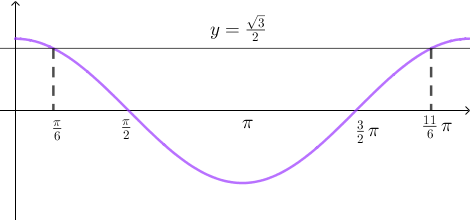
\includegraphics[width=.7\textwidth]{equa_1-3}
\end{center}
\newpage
\item
\(y=\tan x\)의 그래프와 \(y=\sqrt3\)의 교점을 구하면
\(x=\frac\pi3,\quad\frac43\pi\)
\begin{center}
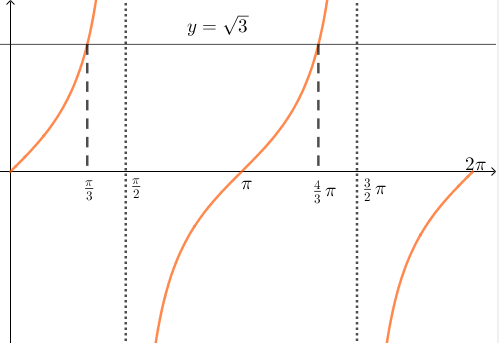
\includegraphics[width=.7\textwidth]{equa_1-4}
\end{center}
\end{enumerate}
\end{mdframed}

%
\exam{\(x\)가 실수일 때, 다음 방정식의 근을 구하여라.}\label{equa2}
\begin{enumerate*}[itemjoin=\tabto{.5\textwidth}]
\item
\(\cos x=\frac{\sqrt3}2\)
\item
\(\tan x=\sqrt3\)
\end{enumerate*}
\begin{mdframed}
\begin{enumerate}
\item
코사인함수는 주기가 \(2\pi\)이므로 \(x=\frac\pi6\)이 방정식 \(\cos x=\frac{\sqrt3}2\)의 근이면
\vspace{-5pt}
\[\textstyle x=\cdots\;,\;\;\;\frac\pi6-2\pi\;,\;\;\;\frac\pi6\;,\;\;\;\frac\pi6+2\pi\;,\;\;\;\frac\pi6+4\pi\;,\;\;\;\cdots\]
의 값들도 근이 된다.
마찬가지로 \(x=\frac{11}6\)가 근이므로
\[\textstyle x=\cdots\;,\;\;\;\frac{11}6\pi-2\pi\;,\;\;\;\frac{11}6\pi\;,\;\;\;\frac{11}6\pi+2\pi\;,\;\;\;\frac{11}6\pi+4\pi\;,\;\;\;\cdots\]
또한 근이 된다.
이것들을 정리하면
\[\textstyle x=\frac\pi6+2n\pi\;,\;\;\;\frac{11}6\pi+2n\pi\;\;(n\text{은 정수})\]
\item
탄젠트함수는 주기가 \(\pi\)이므로
\[\textstyle x=\frac\pi3+n\pi\;,\;\;\;\frac43\pi+n\pi\;\;(n\text{은 정수})\]
\end{enumerate}
\end{mdframed}

%
\prob{\(x\)가 실수일 때, 다음 방정식의 근을 구하여라.}\label{equa3}
\begin{enumerate*}[itemjoin=\tabto{.5\textwidth}]
\item
\(\sin x=-\frac12\)
\item
\(\tan x=1\)
\end{enumerate*}

%%%
\section{삼각부등식}
%
\exam{\(0\le x<2\pi\)일 때, 다음 부등식의 근을 구하여라.}\label{ineq1}
\begin{enumerate*}[itemjoin=\tabto{.5\textwidth}]
\item
\(\cos x<\frac{\sqrt3}2\)
\item
\(\tan x\ge\sqrt3\)
\end{enumerate*}

\begin{mdframed}[frametitle=삼각함수의 정의를 사용하는 방법]
\begin{enumerate}
\item
\par\noindent
\begin{minipage}[t]{.5\textwidth}
원 \(x^2+y^2=1\) 위의 점 \(P(x,y)\) 중 \(x<\frac{\sqrt3}2\)인 점들을 표시하면 오른쪽 그림과 같다.
따라서
\[\frac\pi6<x<\frac{11}6\pi\]
\end{minipage}
\begin{minipage}{.4\textwidth}\centering
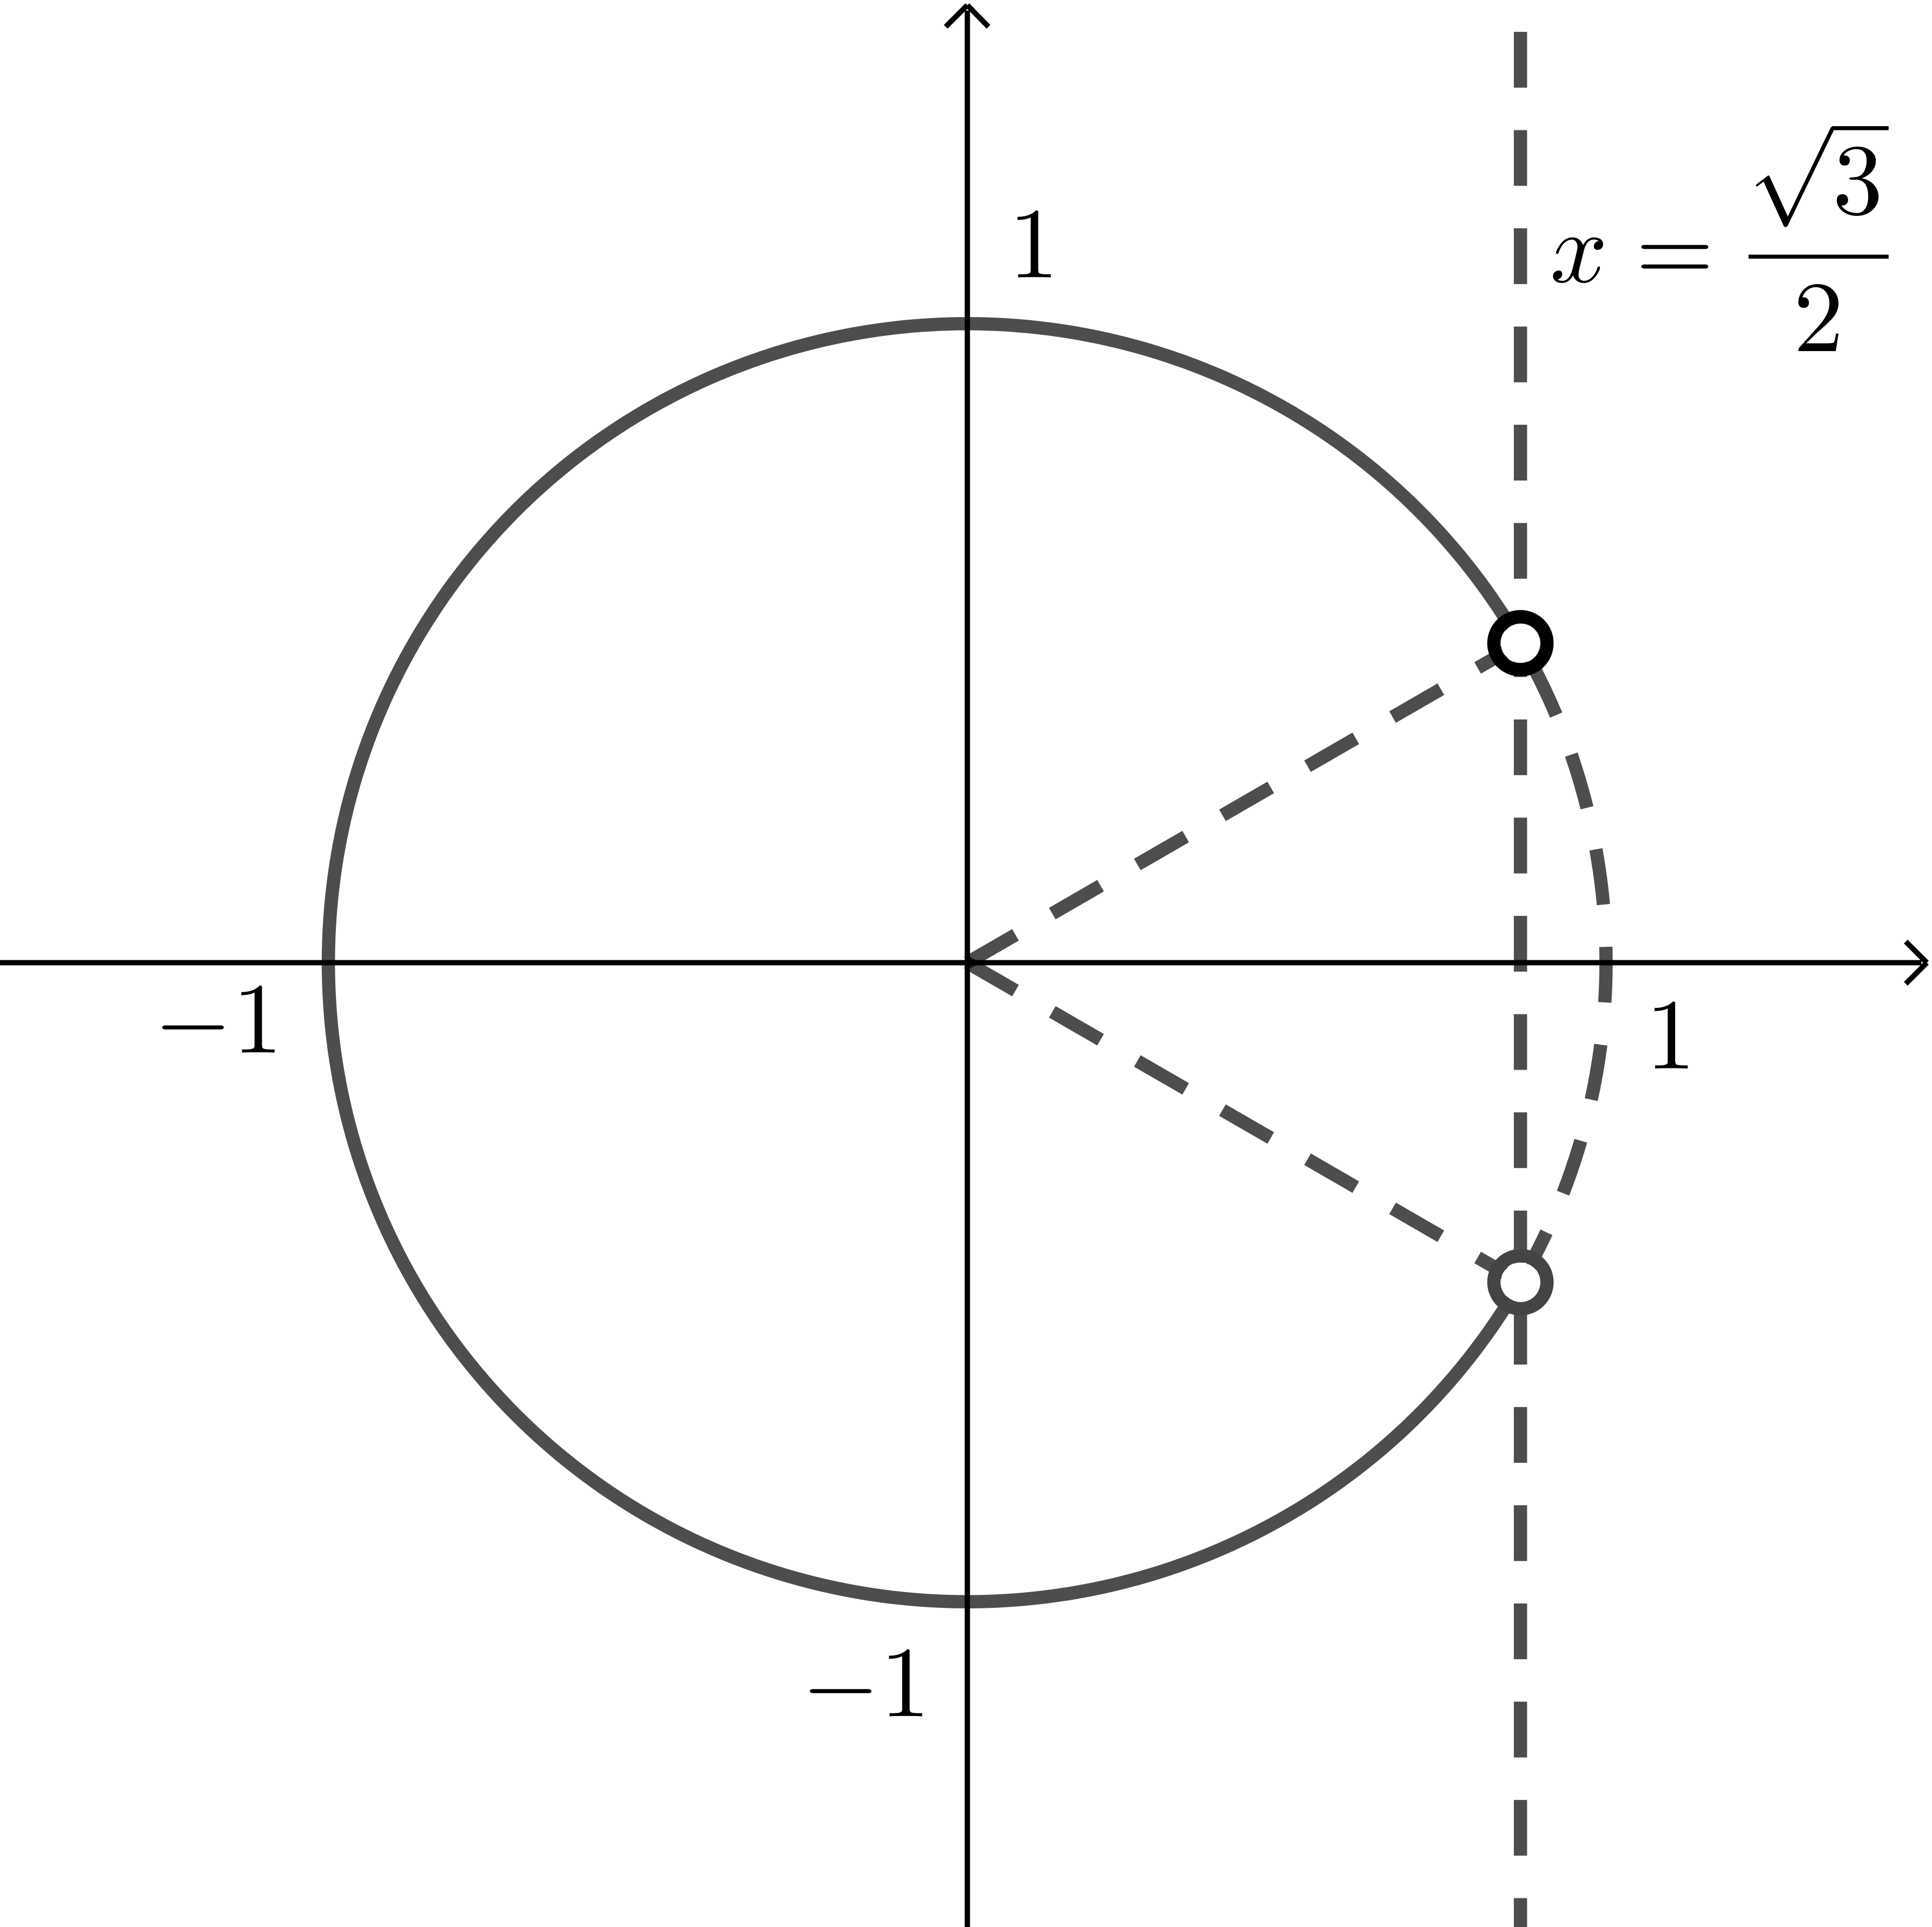
\includegraphics[width=.6\textwidth]{ineq_1-1}
\end{minipage}
\item
\par\noindent
\begin{minipage}[t]{.5\textwidth}
원 \(x^2+y^2=1\) 위의 점 \(P(x,y)\) 중 직선 \(OP\)의 기울기가 \(\sqrt3\)보다 크거나 같은 점들을 표시하면 오른쪽 그림과 같다.
\[x=\frac\pi3,\quad\frac43\pi\]
\end{minipage}
\begin{minipage}{.4\textwidth}\centering
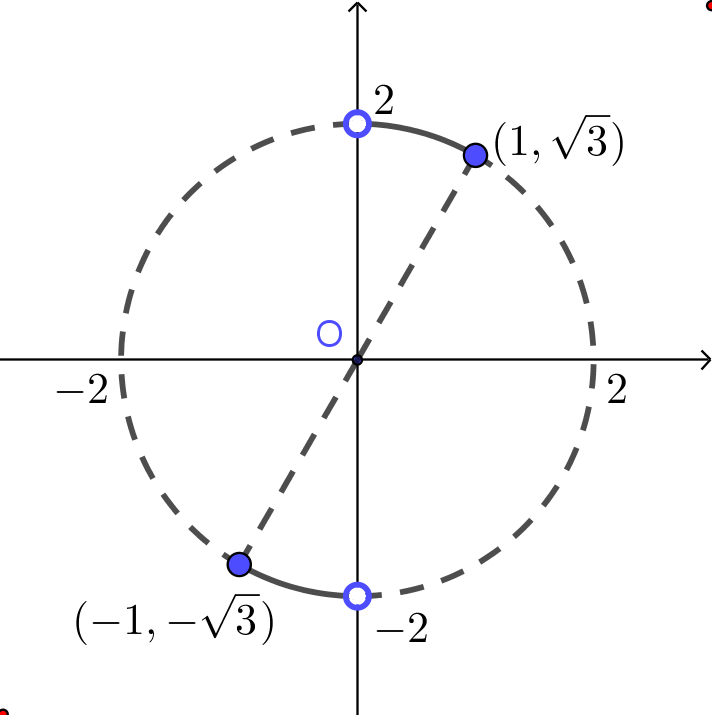
\includegraphics[width=.6\textwidth]{ineq_1-2}
\end{minipage}
\end{enumerate}
\end{mdframed}

\begin{mdframed}[frametitle=그래프를 사용하는 방법,nobreak=false]
\begin{enumerate}
\item
\(y=\cos x\)의 그래프의 부분 중 직선 \(y=\frac{\sqrt3}2\)보다 아래쪽에 있는 부분을 표시하면 다음과 같다.
\begin{center}
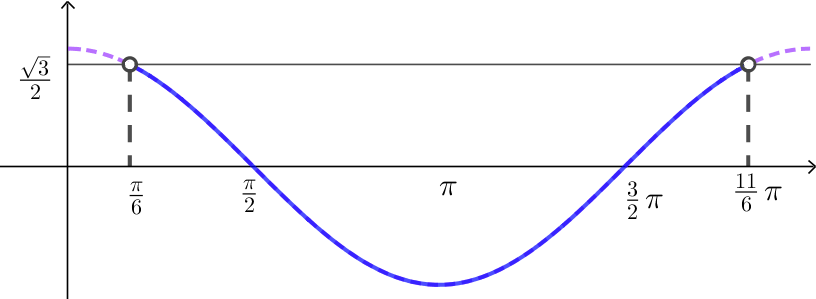
\includegraphics[width=.7\textwidth]{ineq_1-3}
\end{center}
따라서
\[\frac\pi6<x<\frac{11}6\pi\]
\newpage
\item
\(y=\tan x\)의 그래프의 부분 중 직선 \(y=\sqrt3\)보다 위에 있는 부분을 표시하면 다음과 같다.
\begin{center}
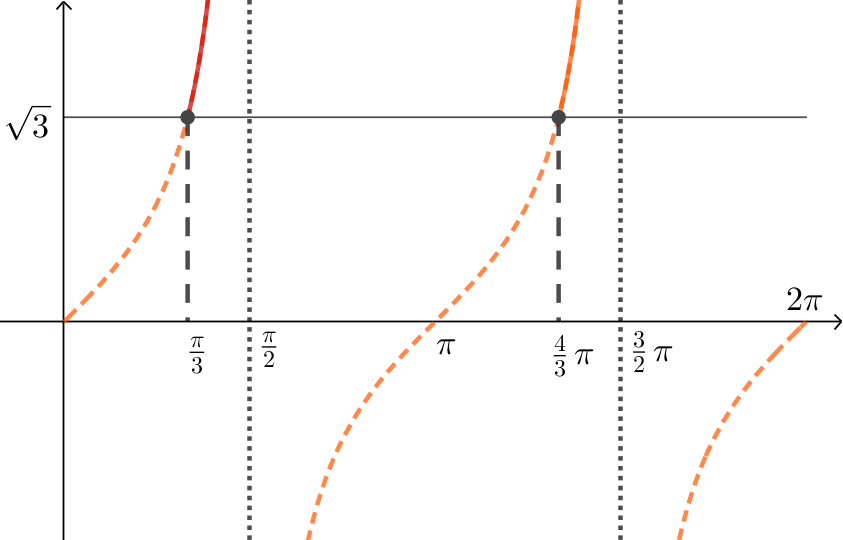
\includegraphics[width=.7\textwidth]{ineq_1-4}
\end{center}
따라서
\[\frac\pi3\le x\le\frac\pi2,\quad\frac43\pi\le x\le\frac32\pi\]
\end{enumerate}
\end{mdframed}

%
\prob{\(0\le x<2\pi\)일 때, 다음 부등식의 근을 구하여라.}\label{ineq2}
\begin{enumerate*}[itemjoin=\tabto{.5\textwidth}]
\item
\(\sin x<-\frac12\)
\item
\(\tan x\le1\)
\end{enumerate*}

%%%
\section{사인법칙}

%
\revi{삼각형의 외심}\label{sin1}
다음은 삼각형의 외심에 대한 설명이다.
문장들을 완성하여라.
\begin{mdframed}
\begin{itemize}
\item
삼각형 \(ABC\)의 외심 \(O\)는 삼각형의 ( 내접원 / 외접원 )의 중심을 말한다.
\item
외심 \(O\)는 (세 각의 각이등분선의 교점 / 세 변의 수직이등분선의 교점 / 중선의 교점 )이기도 하다.
\item
\begin{minipage}[t]{.6\textwidth}
오른쪽 그림에서 \(\triangle OBD\)와 합동인 삼각형은 ( \(\triangle OBF\) / \(\triangle OCD\) )이다.
\vspace{30pt}
\end{minipage}
\begin{minipage}{.3\textwidth}
\begin{center}
\includegraphics[width=.8\textwidth]{sin_1}
\end{center}
\end{minipage}
\item
\(\triangle ABC\)가 예각삼각형이면 점 \(O\)는 삼각형의 ( 내부 / 외부 )에 있다.
\item
\(\triangle ABC\)가 둔각삼각형이면 점 \(O\)는 삼각형의 ( 내부 / 외부 )에 있다.
\item
\(\triangle ABC\)가 직각삼각형이면 점 \(O\)는 \pb{빗변의 중점}에 있다.
\end{itemize}
\end{mdframed}

\bigskip\bigskip
삼각형 \(ABC\)의 세 변의 길이를 각각 \(a\), \(b\), \(c\)라고 할 때, 외접원의 반지름의 길이를 \(R\)이라고 하면 다음 식이 성립한다.
\begin{mdframed}
%
\theo{사인법칙}\label{sin2}
\begin{minipage}[c]{.6\textwidth}
\[\frac a{\sin A}=\frac b{\sin B}=\frac c{\sin C}=2R\]
\end{minipage}
\begin{minipage}{.3\textwidth}
\begin{center}
\includegraphics[width=\textwidth]{sin_2}
\end{center}
\end{minipage}
\end{mdframed}

\newpage
%
\prob{다음은 삼각형 \(ABC\)가 예각삼각형일 때, 사인법칙을 증명하는 과정이다.
빈 칸에 알맞은 것을 써넣어라.}\label{sin3}
\\[-30pt]
\begin{mdframed}
\begin{minipage}{.6\textwidth}
선분 \(BO\)의 연장선이 원과 만나는 점을 \(A'\)이라고 하면
%점 \(A\)를 원을 따라 움직여 세 점 \(A\), \(O\), \(B\)가 한 직선 위에 있도록 하는 점 \(A\)를 \(A'\)이라고 하자.
%그러면
\(\angle A\)와 \(\angle A'\)은 모두 호 \(BC\)에 대한 원주각이므로
\[\angle A=\angle A'\]
\end{minipage}
\begin{minipage}{.4\textwidth}
\centering
\includegraphics[width=.7\textwidth]{sin_3}
\end{minipage}\\
그러면 \(\triangle A'BC\)는 직각삼각형이므로
\[\sin A'=\frac{\:\:\fbox{(가)}\:\:}{2R}\]
따라서
\[\frac{\:\:\fbox{(가)}\:\:}{\sin A}=2R\]
이다.
마찬가지의 방법을 활용하면
\[\frac{\:\:\fbox{(나)}\:\:}{\sin B}=2R,
\quad
\frac{\:\:\fbox{(다)}\:\:}{\sin C}=2R\]
이다.
따라서 사인법칙이 증명되었다.
\end{mdframed}

\vspace{-20pt}
%
\prob{다음 그림에서 \(a\), \(R\), \(\theta\)를 차례로 구하여라.}\label{sin4}
\begin{minipage}{.2\textwidth}\centering
\includegraphics[width=\textwidth]{sin_4-1}
\\\(a=\)
\end{minipage}
\qquad
\begin{minipage}{.2\textwidth}\centering
\includegraphics[width=\textwidth]{sin_4-2}
\\\(R=\)
\end{minipage}
\qquad
\begin{minipage}{.2\textwidth}\centering
\includegraphics[width=\textwidth]{sin_4-3}
\\\(\theta=\)
\end{minipage}

\noindent
\begin{minipage}{.6\textwidth}
%
\prob{오른쪽 그림에서 \(b\)의 값을 구하여라.}\label{sin5}
\vspace{30pt}
\mbox{}
\end{minipage}
\begin{minipage}{.4\textwidth}
\centering
\includegraphics[width=.6\textwidth]{sin_5}
\end{minipage}

%%%
\section{코사인법칙}

%
\revi{피타고라스 정리의 역}\label{cos1}
삼각형 \(ABC\)의 세 꼭짓점의 대변의 길이가 각각 \(a\), \(b\), \(c\)일 때,
다음 빈칸에 알맞은 등호(\(=\)) 혹은 부등호(\(<\), \( >\))를 써넣어라.
\begin{mdframed}
\begin{itemize}
\item
\(\angle C\)가 예각이면 \(a^2+b^2\;\pb{=}\; c^2\)이다.
\item
\(\angle C\)가 직각이면 \(a^2+b^2\;\pb{<}\; c^2\)이다.
\item
\(\angle C\)가 둔각이면 \(a^2+b^2\;\pb{>}\; c^2\)이다.
\end{itemize}
\end{mdframed}

\bigskip\bigskip
삼각형 \(ABC\)에 대하여 다음 정리가 성립한다.
\begin{mdframed}
%
\theo{코사인법칙}\label{cos2}
\begin{minipage}[c]{.6\textwidth}
\begin{align*}
a^2&=b^2+c^2-2bc\cos A\\
b^2&=c^2+a^2-2ca\cos B\\
c^2&=a^2+b^2-2ab\cos C
\end{align*}
\end{minipage}
\begin{minipage}{.3\textwidth}
\begin{center}
\includegraphics[width=\textwidth]{cos_2}
\end{center}
\end{minipage}
\end{mdframed}

%
\prob{\(\angle B\)가 예각일 때, 코사인법칙을 증명하는 과정이다.
빈 칸에 알맞은 선을 써넣어라.}\label{cos3}
\begin{mdframed}[nobreak=false]
\begin{minipage}{.6\textwidth}
점 \(A\)에서 선분 \(BC\)에 내린 수선의 발을 \(H\)라고 하면
\(\sin B=\frac{\ov AH}c\),
\(\cos B=\frac{\ov BH}c\)
이다.
따라서
\[\ov AH=\fbox{(가)},\quad \ov BH=\fbox{(나)}\]
한편 \(\ov CH=\ov BC-\ov BH\)이므로
\[\ov CH=a-\fbox{(나)}\]
\end{minipage}
\begin{minipage}{.4\textwidth}
\centering
\includegraphics[width=.7\textwidth]{cos_3}
\end{minipage}\\
직각삼각형 \(AHC\)에 피타고라스의 정리를 적용시키면 \(\ov AC^2=\ov AH^2+\ov CH^2\)으로부터
\[b^2=\fbox{(가)}^2+\left(a-\fbox{(나)}\right)^2\]
이 식을 정리하면
\[b^2=c^2+a^2-2ca\cos B\]
이 얻어진다.
마찬가지의 방법을 사용하면
\begin{align*}
a^2&=b^2+c^2-2bc\cos A\\
c^2&=a^2+b^2-2ab\cos C
\end{align*}
도 얻을 수 있다.
\end{mdframed}

\noindent
\begin{minipage}{.6\textwidth}
%
\prob{오른쪽 그림에서 \(a\)의 값을 구하여라.}\label{cos4}
\vspace{30pt}
\mbox{}
\end{minipage}
\begin{minipage}{.4\textwidth}
\centering
\includegraphics[width=.6\textwidth]{cos_4}
\end{minipage}

\noindent
\begin{minipage}{.6\textwidth}
%
\prob{오른쪽 그림에서 \(\cos C\)의 값을 구하여라.}\label{cos5}
\vspace{30pt}
\mbox{}
\end{minipage}
\begin{minipage}{.4\textwidth}
\centering
\includegraphics[width=.6\textwidth]{cos_5}
\end{minipage}

%
\prob{다음 그림에서 \(\ov AB=4\), \(\ov BC=5\)이다.
\(\angle B\)가 각각 \(60^\circ\), \(90^\circ\), \(120^\circ\)일 때, \(\ov AC\)의 길이를 차례로 구하여라.}\label{cos6}
\begin{minipage}{.24\textwidth}\centering
\includegraphics[width=\textwidth]{cos_6-1}
\\\(\ov AC=\)
\end{minipage}
\qquad
\begin{minipage}{.24\textwidth}\centering
\includegraphics[width=\textwidth]{cos_6-2}
\\\(\ov AC=\)
\end{minipage}
\qquad
\begin{minipage}{.32\textwidth}\centering
\includegraphics[width=\textwidth]{cos_6-3}
\\\(\ov AC=\)
\end{minipage}

%%%
\section*{답}
\addcontentsline{toc}{chapter}{\protect\numberline{*}답}
%\begin{multicols*}{2}
%
\ann{rad1}{
\begin{enumerate*}[itemjoin=\qquad]
\item
\(2.54\times3\)
\item
\(\frac1{2.54}\)
\item
\(\frac4{2.54}\)
\end{enumerate*}}

%
\an{rad4}
\begin{tabu}{|X[c$]|X[c$]|X[c$]|X[c$]|X[c$]|X[c$]|X[c$]|X[c$]|X[c$]|X[c$]|X[c$]|}
\hline
 0\textdegree{}
&30\textdegree{}
&45\textdegree{}
&60\textdegree{}
&90\textdegree{}
&120\textdegree{}
&135\textdegree{}
&150\textdegree{}
&180\textdegree{}
&270\textdegree{}
&360\textdegree{}
\\\hline
0
&\frac\pi6
&\frac\pi4
&\frac\pi3
&\frac\pi2
&\frac23\pi
&\frac34\pi
&\frac56\pi
&\pi
&\frac32\pi
&2\pi
\\\hline
\end{tabu}

%
\ann{arc1}{\(l=\frac52\pi\), \(S=\frac{25}2\pi\)}

%
\ann{arc5}{
\begin{enumerate*}[itemjoin=\qquad]
\item
\(l=\pi\), \(S=3\pi\)
\item
\(l=\frac{20}3\pi\), \(S=\frac{100}3\pi\)
\end{enumerate*}
}

%
\ann{arc6}{\(\frac34\pi\)}

%
\an{tratio3}
\begin{enumerate}
\item
\(\sin\frac\pi6=\frac12\),\quad			\(\cos\frac\pi6=\frac{\sqrt3}2\),\quad	\(\tan\frac\pi6=\frac{\sqrt3}3\)
\item
\(\sin\frac\pi4=\frac{\sqrt2}2\),\quad	\(\cos\frac\pi4=\frac{\sqrt2}2\),\quad	\(\tan\frac\pi4=1\)
\end{enumerate}

%
\ann{tratio4}{1, 1}

%
\ann{tratio5}{
\(\fbox{(가)}=\ov CP\),
\(\fbox{(나)}=\ov AD\),
\(\fbox{(다)}=\ov OC\)}
\begin{enumerate}
\item
\(\sin0=0\),\quad		\(\cos0=1\),\quad		\(\tan0=0\)
\item
\(\sin\frac\pi2=1\),\quad	\(\cos\frac\pi2=0\),\quad	\(\tan\frac\pi2=\text{\scriptsize(존재하지 않는다.)}\)
\end{enumerate}

%
\an{tfunction3}
\noindent
\begin{minipage}{.25\textwidth}
\begin{talign*}
\sin\frac\pi4&=\frac{\sqrt2}2\\
\cos\frac\pi4&=\frac{\sqrt2}2\\
\tan\frac\pi4&=1
\end{talign*}
\end{minipage}
\begin{minipage}{.25\textwidth}
\begin{talign*}
\sin\frac23\pi&=\frac{\sqrt3}2\\
\cos\frac23\pi&=-\frac12\\
\tan\frac23\pi&=-\sqrt3
\end{talign*}
\end{minipage}
\begin{minipage}{.25\textwidth}
\begin{talign*}
\sin\frac73\pi&=\frac{\sqrt3}2\\
\cos\frac73\pi&=\frac12\\
\tan\frac73\pi&=\sqrt3
\end{talign*}
\end{minipage}
\begin{minipage}{.25\textwidth}
\begin{talign*}
\sin(-\pi)&=0\\
\cos(-\pi)&=-1\\
\tan(-\pi)&=0
\end{talign*}
\end{minipage}

%
\ann{property2}{
\begin{enumerate*}[itemjoin=\qquad]
\item
\(\frac12\)
\item
\(\pm\frac13\)
\item
\(\frac34\)
\item
\(\frac{\sqrt{21}}2\)
\end{enumerate*}
}


%
\an{property4}
\noindent
\begin{minipage}{.25\textwidth}
\begin{talign*}
\sin(\theta+4\pi)&=\frac{12}{13}\\
\cos(\theta+4\pi)&=\frac5{13}\\
\tan(\theta+4\pi)&=\frac{12}5
\end{talign*}
\end{minipage}
\begin{minipage}{.25\textwidth}
\begin{talign*}
\sin(-\theta)&=-\frac{12}{13}\\
\cos(-\theta)&=\frac5{13}\\
\tan(-\theta)&=-\frac{12}5
\end{talign*}
\end{minipage}
\begin{minipage}{.25\textwidth}
\begin{talign*}
\sin(\theta+\pi)&=-\frac{12}{13}\\
\cos(\theta+\pi)&=-\frac5{13}\\
\tan(\theta+\pi)&=\frac{12}5
\end{talign*}
\end{minipage}
\begin{minipage}{.25\textwidth}
\begin{talign*}
\sin(\frac\pi2-\theta)&=\frac5{13}\\
\cos(\frac\pi2-\theta)&=\frac{12}{13}\\
\tan(\frac\pi2-\theta)&=\frac5{12}
\end{talign*}
\end{minipage}

%
\an{graph1}
\begin{tabu}{|@{}X[2c$]@{}|@{}X[c$]@{}|@{}X[c$]@{}|@{}X[c$]@{}|@{}X[c$]@{}|@{}X[c$]@{}|@{}X[c$]@{}|@{}X[c$]@{}|@{}X[c$]@{}|@{}X[c$]@{}|@{}X[c$]@{}|@{}X[c$]@{}|@{}X[c$]@{}|@{}X[c$]@{}|}
\hline
\theta
&0
&\frac\pi6
&\frac\pi3
&\frac\pi2
&\frac23\pi
&\frac56\pi
&\pi
&\frac76\pi
&\frac43\pi
&\frac32\pi
&\frac53\pi
&\frac{11}6\pi
&2\pi
\\\hline
\sin\theta
&0
&\frac12
&\frac{\sqrt3}2
&1
&\frac{\sqrt3}2
&\frac12
&0
&-\frac12
&-\frac{\sqrt3}2
&-1
&-\frac{\sqrt3}2
&-\frac12
&0
\\\hline
\cos\theta
&1
&\frac{\sqrt3}2
&\frac12
&0
&-\frac12
&-\frac{\sqrt3}2
&-1
&-\frac{\sqrt3}2
&-\frac12
&0
&\frac12
&\frac{\sqrt3}2
&1
\\\hline
\tan\theta
&0
&\frac{\sqrt3}3
&\sqrt3
&\times
&-\sqrt3
&-\frac{\sqrt3}3
&0
&\frac{\sqrt3}3
&\sqrt3
&\times
&-\sqrt3
&-\frac{\sqrt3}3
&0
\\\hline
\end{tabu}
\par\noindent
\(\times\) : 존재하지 않음
%\par\bigskip\noindent
%위의 표를 참고하여 \(y=\sin x\), \(y=\cos x\), \(y=\tan x\)의 그래프를 그려라.%}\label{graph2}
\newpage
\begin{figure*}[h!]
\centering
\includegraphics[width=.9\textwidth]{graph_1-1}
\caption*{\(y=\sin x\)}
\end{figure*}

\begin{figure*}[h!]
\centering
\includegraphics[width=.9\textwidth]{graph_1-2}
\caption*{\(y=\cos x\)}
\end{figure*}

\begin{figure*}[h!]
\centering
\includegraphics[width=.9\textwidth]{graph_1-3}
\caption*{\(y=\tan x\)}
\end{figure*}

%
\an{graph4}
\begin{enumerate}
\item
\(y=2\sin x\)
\end{enumerate}
\par\noindent
\begin{tabu}{|@{}X[2c$]@{}|@{}X[c$]@{}|@{}X[c$]@{}|@{}X[c$]@{}|@{}X[c$]@{}|@{}X[c$]@{}|@{}X[c$]@{}|@{}X[c$]@{}|@{}X[c$]@{}|@{}X[c$]@{}|@{}X[c$]@{}|@{}X[c$]@{}|@{}X[c$]@{}|@{}X[c$]@{}|}
\hline
x&0&\frac\pi6&\frac\pi3&\frac\pi2&\frac23\pi&\frac56\pi&\pi&\frac76\pi&\frac43\pi&\frac32\pi&\frac53\pi&\frac{11}6\pi&2\pi
\\\hline
2\sin x
&0
&1
&\sqrt3
&2
&\sqrt3
&1
&0
&-1
&-\sqrt3
&-2
&-\sqrt3
&-1
&0
\\\hline
\end{tabu}
\begin{figure*}[h!]
\centering
\includegraphics[width=\textwidth]{graph_4-1}
\end{figure*}
\begin{enumerate}
\stepcounter{enumi}
\item
\(y=\sin 2x\)
\end{enumerate}
\par\noindent
\begin{tabu}{|@{}X[2c$]@{}|@{}X[c$]@{}|@{}X[c$]@{}|@{}X[c$]@{}|@{}X[c$]@{}|@{}X[c$]@{}|@{}X[c$]@{}|@{}X[c$]@{}|@{}X[c$]@{}|@{}X[c$]@{}|@{}X[c$]@{}|@{}X[c$]@{}|@{}X[c$]@{}|@{}X[c$]@{}|}
\hline
x&0&\frac\pi6&\frac\pi3&\frac\pi2&\frac23\pi&\frac56\pi&\pi&\frac76\pi&\frac43\pi&\frac32\pi&\frac53\pi&\frac{11}6\pi&2\pi
\\\hline
\sin 2x
&0
&\frac{\sqrt3}2
&\frac{\sqrt3}2
&0
&-\frac{\sqrt3}2
&-\frac{\sqrt3}2
&0
&\frac{\sqrt3}2
&\frac{\sqrt3}2
&0
&-\frac{\sqrt3}2
&-\frac{\sqrt3}2
&0
\\\hline
\end{tabu}
\begin{figure*}[h!]
\centering
\includegraphics[width=\textwidth]{graph_4-2}
\end{figure*}

\newpage

\ann{equa3}{
\begin{enumerate*}[itemjoin=\qquad\qquad]
\item
\(x=\frac76\pi+2n\pi,\quad\frac{11}6\pi+2n\pi\)
\item
\(x=\frac\pi4+n\pi,\quad\frac54\pi+n\pi\)
\end{enumerate*}
}

%
\ann{ineq2}{
\begin{enumerate*}[itemjoin=\qquad\qquad]
\item
\(\frac23\pi<x<\frac43\pi\)
\item
\(0\le x\le\frac\pi4\), \(\frac\pi2<x\le\frac54\pi\), \(\frac32\pi<x<2\pi\)
\end{enumerate*}
}
%
\an{sin1}
\begin{itemize}
\item
외접원
\item
세 변의 수직이등분선의 교점
\item
\(\triangle OCD\)
\item
내부
\item
외부
\item
빗변의 중점
\end{itemize}

%
\ann{sin3}{
\(\fbox{(가)}=a\), \(\fbox{(나)}=b\), \(\fbox{(다)}=c\)
}

%
\ann{sin4}{
\begin{enumerate*}[itemjoin=\qquad\qquad]
\item
\(10\sqrt2\)
\item
5
\item
\(60\textdegree{}(=\frac\pi3)\)
\end{enumerate*}
}

%
\ann{sin4}{\(\frac{8\sqrt6}3\)}

\newpage
%
\ann{cos1}{\(>\), \(=\), \(<\)}

%
\ann{cos3}{\(\fbox{(가)}=\ov AH\), \(\fbox{(나)}=\ov BH\)}

%
\ann{cos4}{\(\sqrt{13}\)}

%
\ann{cos5}{\(\frac34\)}

%
\ann{cos6}{\(\sqrt{21}\), \(\sqrt{41}\), \(\sqrt{61}\)}

\newpage
\mbox{}
\newpage
\mbox{}

%\end{multicols*}

%
\section*{요약}
\addcontentsline{toc}{chapter}{\protect\numberline{*}요약}
\begin{enumerate}[label=\arabic*]
%\item
%호도법
\stepcounter{enumi}
\item
부채꼴의 호의 길이와 넓이
\[l=r\theta,\quad S=\frac12r^2\theta=\frac12rl\]
\stepcounter{enumi}
\item
삼각함수\\
\noindent\begin{minipage}{.6\textwidth}
%동경 \(OP\)가 나타내는 일반각 \(\theta\)에 대하여
\[\sin\theta=\frac yr,\quad\cos\theta=\frac xr,\quad\tan\theta=\frac yx\]
\end{minipage}
\begin{minipage}{.4\textwidth}
\centering
\includegraphics[width=.8\textwidth]{summary_4}
\end{minipage}
\item
삼각함수의 성질
\begin{gather*}
-1\le\sin x\le1,\quad-1\le\cos x\le1\\
\sin^2x+\cos^2x=1\\
\tan x=\frac{\sin x}{\cos x}%\\
%\sin(x+2\pi)=\sin x,\quad\cos(x+2\pi)=\cos x,\quad\tan(x+\pi)=\tan x\\
%\sin(-x)=-\sin x,\quad\cos(-x)=\cos x,\quad\tan(-x)=-\tan x\\
%\sin(\frac\pi2-x)=\cos x,\quad\cos(\frac\pi2-x)=\sin x,\quad\tan(\frac\pi2-x)=\frac1{\tan x}
\end{gather*}
%\stepcounter{enumi}
\item
삼각함수의 그래프
\begin{center}
\includegraphics[width=.25\textwidth]{summary_6-1}\qquad
\includegraphics[width=.25\textwidth]{summary_6-2}\qquad
\includegraphics[width=.25\textwidth]{summary_6-3}
\par
\begin{tabu}{X[c]X[c]X[c]}
\(y=\sin x\)&\(y=\cos x\)&\(y=\tan x\)
\end{tabu}
\end{center}
\stepcounter{enumi}
\stepcounter{enumi}
\item
사인법칙
\[\frac a{\sin A}=\frac b{\sin B}=\frac c{\sin C}=2R\]
\item
코사인법칙
\begin{align*}
a^2&=b^2+c^2-2bc\cos A\\
b^2&=c^2+a^2-2ca\cos B\\
c^2&=a^2+b^2-2ab\cos C
\end{align*}
\end{enumerate}
\end{document}